\documentclass[UTF8]{pkuthss}
\usepackage[backend = biber, style = caspervector, utf8, sorting = none]{biblatex}
\usepackage{multirow}
\usepackage{booktabs}
\usepackage {colortbl}
\setlength{\bibitemsep}{3bp}
\renewcommand*{\bibfont}{\zihao{5}\linespread{1.27}\selectfont}
\pkuthssinfo{
	cthesisname = {硕士研究生学位论文}, ethesisname = {Master Thesis},
	ctitle = {实时区块链实名交易监督系统的设计与实现}, etitle = {Design and Implementation of Real-time Blockchain Real-name Transaction Monitoring System},
	cauthor = {陈伯韦},
	eauthor = {Chen Po Wei},
	studentid = {1601210903},
	date = {二〇一八 年 七 月 },
	school = {软件与微电子学院},
	cmajor = {软件工程专业}, emajor = {Data Mining and Business Intelligence},
	direction = {数据挖掘与商务智能方向},
	cmentor = {李杰\ 教授、刘京\ 讲师}, ementor = {Prof.\ Lijie,\ Lecturer\ Liujing},
	ckeywords = {比特币,区块链,多重签章算法}, ekeywords = {Bitcoin, Blockchain, Multiple signatures algorithm}
} 
\addbibresource{thesis.bib}
\usepackage{color}
\def\pkuthssffaq{%
	\emph{\textcolor{red}{pkuthss 文档模版最常见问题:}}
	\texttt{\string\cite}、\texttt{\string\parencite} %
	和 \texttt{\string\supercite} 三个命令分别产生%
	未格式化的、带方括号的和上标且带方括号的引用标记:%
	\cite{test-en},\parencite{test-zh}、\supercite{test-en, test-zh}。

	若要避免章末空白页,请在调用 pkuthss 文档类时加入 \texttt{openany} 选项。

	如果编译时不出参考文献,
	请参考 \texttt{texdoc pkuthss}“问题及其解决”一章
	“其它可能存在的问题”一节中关于 biber 的说明。
}

\begin{document}
	% 以下为正文之前的部分,默认不进行章节编号。
	\frontmatter
	% 此后到下一 \pagestyle 命令之前不排版页眉或页脚。
	\pagestyle{empty}
	% 自动生成封面。
	\maketitle
	% 版权声明。封面要求单面打印,故需新开右页。
	\cleardoublepage
	% Copyright (c) 2008-2009 solvethis
% Copyright (c) 2010-2017 Casper Ti. Vector
% All rights reserved.
%
% Redistribution and use in source and binary forms, with or without
% modification, are permitted provided that the following conditions are
% met:
%
% * Redistributions of source code must retain the above copyright notice,
%   this list of conditions and the following disclaimer.
% * Redistributions in binary form must reproduce the above copyright
%   notice, this list of conditions and the following disclaimer in the
%   documentation and/or other materials provided with the distribution.
% * Neither the name of Peking University nor the names of its contributors
%   may be used to endorse or promote products derived from this software
%   without specific prior written permission.
%
% THIS SOFTWARE IS PROVIDED BY THE COPYRIGHT HOLDERS AND CONTRIBUTORS "AS
% IS" AND ANY EXPRESS OR IMPLIED WARRANTIES, INCLUDING, BUT NOT LIMITED TO,
% THE IMPLIED WARRANTIES OF MERCHANTABILITY AND FITNESS FOR A PARTICULAR
% PURPOSE ARE DISCLAIMED. IN NO EVENT SHALL THE COPYRIGHT HOLDER OR
% CONTRIBUTORS BE LIABLE FOR ANY DIRECT, INDIRECT, INCIDENTAL, SPECIAL,
% EXEMPLARY, OR CONSEQUENTIAL DAMAGES (INCLUDING, BUT NOT LIMITED TO,
% PROCUREMENT OF SUBSTITUTE GOODS OR SERVICES; LOSS OF USE, DATA, OR
% PROFITS; OR BUSINESS INTERRUPTION) HOWEVER CAUSED AND ON ANY THEORY OF
% LIABILITY, WHETHER IN CONTRACT, STRICT LIABILITY, OR TORT (INCLUDING
% NEGLIGENCE OR OTHERWISE) ARISING IN ANY WAY OUT OF THE USE OF THIS
% SOFTWARE, EVEN IF ADVISED OF THE POSSIBILITY OF SUCH DAMAGE.

% 此处不用 \specialchap,因为学校要求目录不包括其自己及其之前的内容。
\chapter*{版权声明}
% 综合学校的书面要求及 Word 模版来看,版权声明页不需加页眉、页脚。
\thispagestyle{empty}

任何收存和保管本论文各种版本的单位和个人,
未经本论文作者同意,不得将本论文转借他人,
亦不得随意复制、抄录、拍照或以任何方式传播。
否则一旦引起有碍作者著作权之问题,将可能承担法律责任。

% 若需排版二维码,请将二维码图片重命名为“barcode”,
% 转为合适的图片格式,并放在当前目录下,然后去掉下面 2 行的注释。
%\vfill\noindent
%\includegraphics[height = 5em]{barcode}

% vim:ts=4:sw=4


	% 此后到下一 \pagestyle 命令之前正常排版页眉和页脚。
	\cleardoublepage
	\pagestyle{plain}
	% 重置页码计数器,用大写罗马数字排版此部分页码。
	\setcounter{page}{0}
	\pagenumbering{Roman}
	% 中英文摘要。

	% Copyright (c) 2014,2016 Casper Ti. Vector
% Public domain.

\begin{cabstract}
	%\pkuthssffaq % 中文测试文字
	金融科技蓬勃發展的今天,區塊鏈技術也是重點發展對象。區塊鏈技術最著名的代表作,不外乎是於2009年中本聰提出的一篇名為比特幣:一種點對點式的電子現金系統》(Bitcoin: A Peer-to-Peer Electronic Cash System)論文\parencite{bitcoinpaper},奠定了區塊鏈技術的開始,以及於貨幣銀行學緊密的結合。比特幣是一個集成網路學、密碼學、金融學的密碼貨幣,現今的密碼貨幣市場中,有數以千計的貨幣種類在市場流動著。值得一提的是,於2009年開始運作至今(2018年),比特幣點對點式的電子現金系統,還未出現過錯誤,這也體現了比特幣可以承受將近十年來各式各樣的網路攻擊以及在程序上並無太大的漏洞瑕疵。比特幣最大的特色在於去中心化、匿名化,因為去中心化的基礎建構出一個政府無法管控的點對點的金流,也因為匿名,使得政府相關人士難以追查每一筆資金的真正持有者是誰,在傳統的中心化銀行跨國轉帳中都需要基本的實名制驗證,藉由實名制有效過濾洗錢的發生。但在比特幣點對點的電子現金系統中,沒有任何一個使用者或是政府可以要求每一個人的實名制,促使的交易追蹤、洗錢防制變得更加的困難。除了不可管控、難以追蹤的特點外,在國家政府方面稅收更是國家繼續運作的基礎資金來源,因為現今的國家並無支持比特幣相關的收銀機或是制定出相關的標準稅務,也使得國家政府無法在這方面獲得稅務資金。

	經由深度的了解比特幣的運作原理,再由上述無法管理資金流、無法追蹤、無法得到稅收,三項出發點,本論文致力於設計一個比特幣的收銀監督系統。在設計該系統前,也探討了多種場景下的交易模型,發現現金已經存在匿名支付給匿名、匿名支付給實名的模型,在刷卡支付中有著實名支付給實名、實名支付給匿名再支付給實名,上述的四種模型。經由上述的分析,可以得知,個人隱私的意識崛起,唯有匿名支付給實名時,才可以做到不透露消費者信息,亦可做到消費者權益的申訴權。在點對點的電子現金的市場中,還是停留在匿名支付給匿名的場景中,本論文致力於設計一個匿名支付實名的密碼貨幣市場的監督收銀系統,以實踐消費者匿名,同時也讓消費者擁有費者權益的交易模型。
\end{cabstract}

\begin{eabstract}
	Test of the English abstract.
\end{eabstract}

% vim:ts=4:sw=4

	% 自动生成目录。
	\setcounter{tocdepth}{1}
	\tableofcontents

	\renewcommand\listfigurename{图目录}
	\newcommand{\loflabel}{图}
	\renewcommand{\numberline}[1]{\loflabel~#1\hspace*{1em}}
	\listoffigures
	\renewcommand\listtablename{表目录}
	\newcommand{\lotlabel}{表}
	\renewcommand{\numberline}[1]{\lotlabel~#1\hspace*{1em}}
	\listoftables

	%% 以下为正文部分,默认要进行章节编号。
	\mainmatter
	% 序言。
	%% Copyright (c) 2014,2016 Casper Ti. Vector
% Public domain.

\specialchap{序言}
%\pkuthssffaq % 中文测试文字。
現貨法定貨幣,收據及交易數據庫存在著一些缺點。如現貨幣很難杜絕假鈔的橫行,收據有著偽造的可能,在交易數據庫中資料不一致,數據庫被DDOS攻擊,交易數據被竄改,數據庫損毀,也都是在交易過程中曾出現的窘境。

於2009年加密貨幣 - 比特幣的問世,以密碼學、網路學、貨幣銀行學為基礎創建了新一代的網路貨幣。竄改、公開交易數據檢視、使用者匿名性、自動運作不須人為運營的多項特性。至今區塊鏈技術已成為IBM、摩根大通、微軟、谷歌、英特爾重點開發項目,被視為改善銀行運作效率、降低運營成本、提升資訊安全、建立公開數據的最佳方法。為解決現金、收益及交易數據庫存在之問題,預採用以區塊為基礎的數字貨幣比特幣為貨幣,進行商業化收銀系統開發。不僅僅是比特幣算法穩定、交易公開透明、不可被竄改的特性外,更是本論文加入監督標籤,使得在匿名交易轉為部分實名交易,促使監管部門能有更好的貨幣技術提升,亦可建立自動化的稅務審查機制,大幅降地人成本,亦可提高交易系統的信息可靠度及穩定度。
% vim:ts=4:sw=4

	% 各章节。
	% Copyright (c) 2014,2016 Casper Ti. Vect

\chapter{绪论}

	現金法定貨幣,收據及交易數據庫存在著一些缺點。如現金很難杜絕假鈔的橫行,收據有著偽造的可能,在交易數據庫中信息不一致,數據庫被DDOS攻擊,交易數據被竄改,數據庫損毀,都是在傳統交易過程中曾出現過的窘境。

	於2009年加密貨幣 - 比特幣的問世,以密碼學、網絡學與貨幣銀行學為基礎創建了新一代的網絡貨幣。各式網絡貨幣中又以比特幣最為廣泛使用,其防堵被竄改、公開交易數據檢視、使⽤者具匿名性、⾃動運作不須⼈為運營等等多項特性深受現今使用者喜愛。至今區塊鏈技術已成為IBM、摩根大通、微軟、谷歌與英特爾等重點開發項目,被視為改善銀行運作效率、降低運營成本、提升信息安全、建立公開數據的最佳方法。為解決現金、收益及交易數據庫存在之問題,本文採用以區塊鏈為基礎的加密貨幣比特幣為基礎,進行商業化收銀系統開發。不僅是基於⽐特幣算法穩定、交易公開透明、不可被竄改等特性,同時本論⽂更加⼊監督標籤,促使在匿名交易轉為部分實名交易之過程中,監管部⾨能有更好的新興貨幣技術的提升,亦可建立自動化的稅務審查機制,大幅降低人事成本,進而實現提升交易系統信息之可靠度與其穩定性。

	\section{選題背景}

		追溯著加密貨幣市場的演進,於2009年時,比特幣並非第一個加密貨幣,在比特幣之前已經有著很多類似的加密貨幣開發實驗,但是一直無法做出一個穩定點對點式的電子現金系統,關於其製作瓶頸之部分將於後段章節闡述。在比特幣穩定發展之後,有著許多對比特幣有興趣的研究者,以穩定的比特幣系統為基礎修改了許多基本的協議。於2011年相繼創造出了貨幣,將其稱之為⼭寨幣。山寨幣早期較為著名包括有萊特幣(Litecoin,LTC)\supercite{litecoin}、狗幣(Dogecoin,DOGE)\supercite{dogecoin}、域名幣(Namecoin,NMC)\supercite{namecoin},於2014年也有人認為比特幣挖礦使用到了大量的哈希運算,這樣的大量運算也浪費了許多的社會資源,進而開發出較具意義的工作量證明挖礦算法,其中較為著名的如素數幣(Primecoin,XPM)\supercite{primecoin}。 於2015年底也誕生了現在最為著名的以太坊經典(Ethereum Classic,ETC)\supercite{ethereumclassic}、以太坊(Ethereum,ETH)\supercite{ethereum},以太坊最重⼤突破設計在於將編程語⾔虛擬機移植到了區塊鏈架構上,這使得區塊鏈技術不再僅止於點對點的電⼦現⾦系統,也創造出了屬於以太坊的編程語言Solidity\supercite{solidity},使以太坊在虛擬機(Ethereum Virtual Machine,EVM)\supercite{Ethereum:Asecuredecentralisedgeneralisedtransactionledger}中可以使⽤Solidity 創建智能合約,合約可以建構去中心化的應用程序,如去中心化的交易所,將交易所去中心化可以有效的防治DDOS攻擊 \supercite{Bitcoin:Economicstechnologyandgovernance},降低交易所因為黑客攻擊而倒閉的可能性。
		

		\subsection{加密貨幣市場}

		加密貨幣中最具代表性的是比特幣,但除了比特幣之外也存在許多模仿比特幣的加密貨幣,有的是為其利益,有的是鑒於比特幣的各種不足,進而希望藉由其他貨幣改善⽐特幣不夠完美之處。加密貨幣市場中有成千上萬種的加密貨幣,其中較廣為人知的加密貨幣會在Cryptocurrency Market Capitalizations\supercite{CryptocurrencyMarketCapitalizations}的排行榜中出現,截至2018年2月8日該排行榜已經收入了1510種加密貨幣。在Cryptocurrency Market Capitalizations統計的數據當中,可知整體的加密貨幣市場,如圖\ref{TotalMarketCapitalization}所示,於2018年1月7日創下了歷史新高,加密貨幣市場的總市值也高達了829,579,000,000美金,相當於五兆人民幣的總市值。

		\begin{figure}[!htbp]
			\centering
			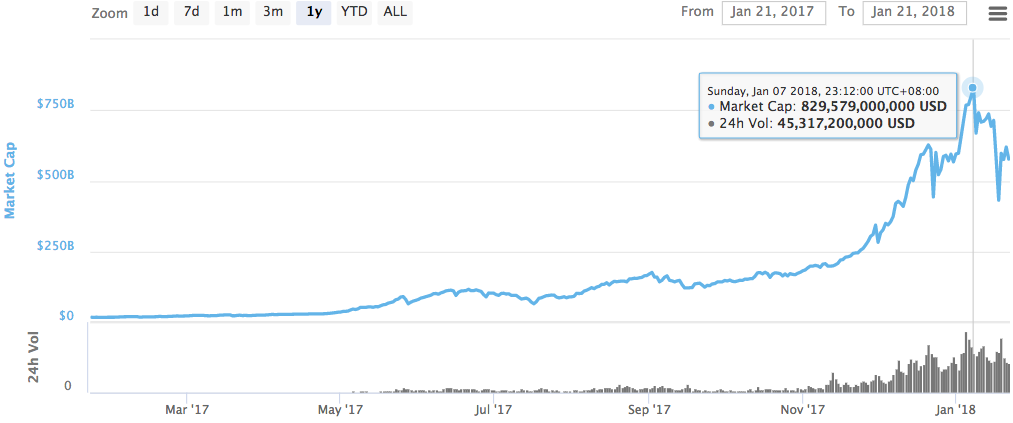
\includegraphics[width = 1\textwidth]{TotalMarketCapitalization.png}
			\caption{2017年1月21日到2018年1月21日期間加密貨幣總市值走勢圖\supercite{CryptocurrencyMarketCapitalizations}}\label{TotalMarketCapitalization}
		\end{figure}

		經由Cryptocurrency Market Capitalizations數據顯示,整體加密貨幣市場自2013年起已經高達150億美金,2014年與2015年間總市值減少到近乎2013年的一半。針對比特幣的價格波動,論文"Have the security flaws surrounding Bitcoin effected the currency's value?."
		\supercite{HavethesecurityflawssurroundingBITCOINeffectedthecurrencysvalue?}
		作出詳盡的市場調研,致力於探討在各個比特幣市場大事件中對比特幣價格的波動影響,針對影響的程度該論文給出影響指數,當中影響最為嚴重的是於2014年2月發生的日本交易所Mt.Gox倒閉事件,因為早期的加密貨幣市場中無完善的法律規範,各國對加密貨幣的接受度有所不同,日本對金融科技的接受度相較於較為開放的情況下成立了全世界第一家比特幣交易所Mt.Gox,也因為交易所不夠普及,使得大部分的加密貨幣交易都集中在Mt.Gox交易所中,使Mt.Gox 倒閉事件成為震盪市場價格重⼤因⼦之⼀,也造成2014與2015年的加密貨幣市場低迷。而在2017年,比特幣又以2016年總市值之35倍的姿態攀上新高點,主要是因為美國最大的期權交易中心芝加哥期權交易所(Chicago Board Options Exchange, CBOE)於2017年12月10日宣布支持比特幣期貨交易,此舉將比特幣價格推升到20,000美金的歷史新高,圖\ref{Thetotalmarketcapitalization}為2013年至2018年歷年的加密貨幣總市值的統計圖表。

			\begin{figure}[!htbp]
				\centering
				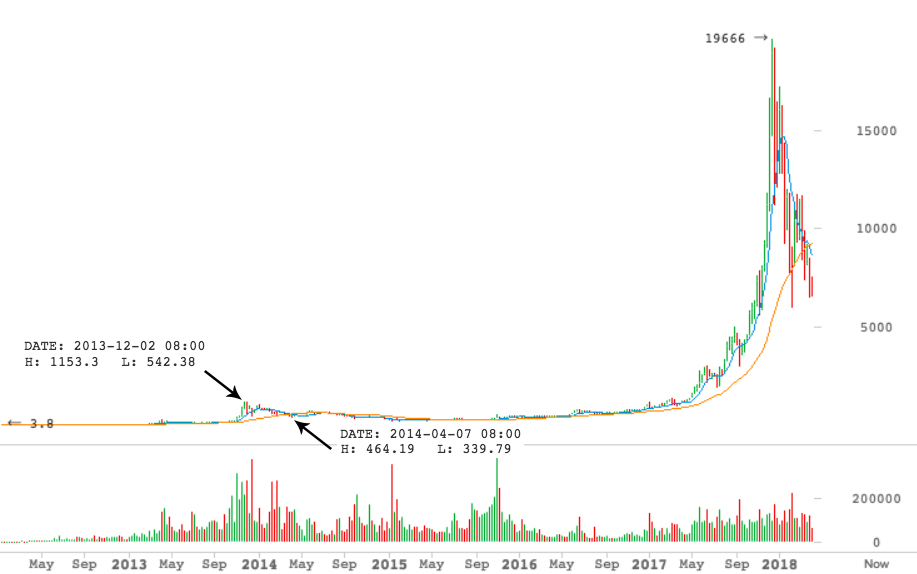
\includegraphics[width = 1\textwidth]{Thetotalmarketcapitalization.jpg}
				\caption{2013年~2018年間比特幣總市值K線圖\supercite{CryptocurrencyMarketCapitalizations}}\label{Thetotalmarketcapitalization}
			\end{figure}
		

			\subsection{加密貨幣的優勢}
			於2009年Satoshi Nakamoto發布了比特幣系統,成為全世界第一個加密貨幣的雛形。其透明的交易信息、區塊鏈交易數據無法修改和刪除、匿名與⾃治系統等特性,促使區塊鏈技術衝破現存傳統中⼼化之⾦融機構技術上的籓籬。以下將逐一說明加密貨幣的七項優點,分別為區塊鏈結算系統不間斷的運行、遠距離支付、貨幣為使用者持有、開放和透明的交易信息、區塊鏈交易數據無法修改和刪除、交易匿名性以及自治性系統。

				第一,區塊鏈結算系統不間斷的運行。基於區塊鏈技術與點對點網絡的架構,以比特幣為例,自2009年至今,所有的比特幣交易事件皆會存儲在比特幣區塊鏈當中,區塊鏈既無法刪除也無法修改,比特幣區塊鏈會以點對點網絡的方式存儲在比特幣網絡中的全節點\supercite{YouReallyShouldRunaBitcoinFullNode:HeresWhy},目前比特幣網絡中的全節點高達10552個。與傳統中心化的銀行數據庫相比,可能會因為銀行的服務器維護,導致交易無法順利進行,甚至可能有黑客的入侵導致銀行或是個人資產有重大的損失。點對點網絡提供穩定的數據庫元數據,不會因為數據庫的停機而無法繼續使用,實現其24小時不間斷之運作。
				
				第二,基於點對點網路架構完成遠距離支付。於跨國匯款從美國轉帳至中國一百萬美金的場景中,需要經過的手續較為繁瑣,資金有可能需要經過多個國家才可以抵達目的地,在經過各個國家的過程中,需要支付各國的手續費,也需要等待各個國家辦理該業務的時間,即使當資金順利抵達了目的地銀行,目的地銀行也需要花將近三至五日的工作日確認該筆金額的來源。屆時領款人亦需要前往銀行核實完整的身份驗證、解釋資金用途,才得以領取這筆跨國資金。比特幣系統當中,有著24小時不間斷運作的優點,也因為點對點網絡架構,使得比特幣無需經由傳統金融機構繁瑣的步驟完成國際匯款,於比特幣系統中無系統壅塞的情況下,平均10分鐘即可入帳,實現其短時間內即可完成遠距離支付之運作。

				第三,加密貨幣為使用者持有。傳統的金融體系中,資金的存儲、流動往往需要經過銀行,使用者將所有的資產存入銀行,拿到的是一串數字的銀行餘額,銀行是一個中心化的機構,有著最高的權利。中央社的新聞\supercite{Bankguardsstolen}指出,臺灣各地於2017年接連於土地銀行、日盛銀行、彰化銀行、京城銀行、兆豐銀行皆傳出銀行行員監守自盜的行為,總金額高達一億三千萬新臺幣。在比特幣系統中,比特幣有如金幣般存放在個人的比特幣地址當中,使用者為真實持有著貨幣,即使是比特幣系統亦無權利動用該筆比特幣資產,唯有比特幣地址的私鑰持有者,才可以轉移該筆比特幣地址中的比特幣資產。

				第四,公開的交易信息。基於區塊鏈架構,所有的交易信息皆以公開的方式存儲於區塊鏈中,並且可信任與方便的取得元數據,以下將針對可信任與元數據進行探討。
				\begin{enumerate}
					\item 可信任:在公有鏈的基本架構上,所有的交易記錄都是公開透明的存儲在區塊鏈當中,比特幣網絡的使用者都可以檢視該筆交易,所有人都可以檢查每個交易記錄的正確性,公開的交易信息亦提升交易數據之可信性。
					\item 元數據:除了以區塊鏈技術為基礎建構出可信任的系統之外,開放和透明的特性讓更多的開發商或新公司得以更容易獲得交易的元數據。畢竟,在傳統金融體系中,所有交易記錄均由中央金融機構存儲,從中央金融機構提取原始交易信息並不容易,區塊鏈的開放性和透明性促使金融公司降低了獲取原始數據努力的門檻。公司或學者可以透過元數據制定出可視化的開發計畫,甚至可以運用大量數據來分析前所未達的新價值觀點。
				\end{enumerate}

				第五,區塊鏈交易數據無法修改和刪除。在區塊鏈結構中,通過嚴格驗證的所有信息都記錄在區塊鏈中,且使用者及系統平台都不賦與刪除及修改之權限。根據區塊鏈的特點,舊區塊的哈希值在連接區塊鏈的過程中,舊區塊的哈希值會被存儲在新區塊。只要區塊中的值被修改,即使僅有1 bit的變化,也會產出完全不同的哈希值,這也就是所謂的雪崩效應(Avalanche effect)\supercite{Theuseofbentsequencestoachievehigher-orderstrictavalanchecriterioninS-boxdesign}。由於上述結構特性,區塊鏈中所有的信息都會被系統紀錄且都不會被改變,倘若區塊中記載的比特幣交易在其中一個比特幣全節點驗證的結果被竄改,則該區塊將不被比特幣系統接受。因此,所有已經存儲在區塊鏈中的交易記錄將不能被修改和刪除,進而實現其架構安全之穩固。

				第六,區塊鏈系統中所有的使用者皆為匿名。現今社會中,個人信息保護已成為企業最重要的課題。在區塊鏈系統中創建的所有帳戶都不會與真實世界中的實體建立直接關聯,也因為沒直接關聯所以建立匿名。區塊鏈系統中的所有帳戶都是由匿名個體創建,匿名的設計可以有效保護消費者的隱私。然而,VISA交易與比特幣系統截然不同,在使用VISA支付系統前,使用者必須向VISA公司的主機提交大量個人信息,這可能會產生個人信息洩露的風險。在區塊鏈技術中,其匿名之特性可以有效地避免這個問題。

				第七,自治系統。在區塊鏈系統中,區塊鏈的運作依賴於一些算法,包括共識算法。因此,在這種自治系統中,沒有人(例如節點或礦工)可以直接改變系統運作的規則。如果在比特幣系統中發現需要更正的嚴重錯誤,可以使用比特幣改進提案(Bitcoin Improvement Proposals,BIP)\supercite{BitcoinImprovementProposals}升級比特幣系統。 在實施比特幣改進提案之前,提議的比特幣改進提案需要得到比特幣系統中超過一定數量的礦工算力支持。由於這種以投票機制升級系統的門檻相當高,使得區塊鏈系統通常不會有大的變化,因為變化不⼤也突顯其相對穩定性。

			\subsection{加密貨幣的劣勢}
			在區塊鏈技術中,有著三項瓶頸,分別為每秒處理的交易量(Transactions Per Second,TPS)僅為七筆的限制、洗錢防治困難、低可擴展性,以下將逐一探討。

				第一,每秒處理的交易量上限僅為7筆。圖\ref{TPS}為國際上較為廣泛使用的⽀付系統之每秒⽀持交易量⽐較圖,以VISA為例,其以公司中心化運營的方式可以支持高達每秒2,000筆交易。但是以區塊鏈技術為基礎的比特幣最大能夠接受的每秒處理交易量僅為7筆。一般認為只要提升區塊大小的限制,就可以提升每秒處理的交易量。提升每秒處理交易量的同時將產生下述的兩項問題,分別為區塊鏈成長速度過快造成節點崩潰以及區塊同步延遲造成區塊鏈分岔:

					\begin{figure}[!htbp]
						\centering
						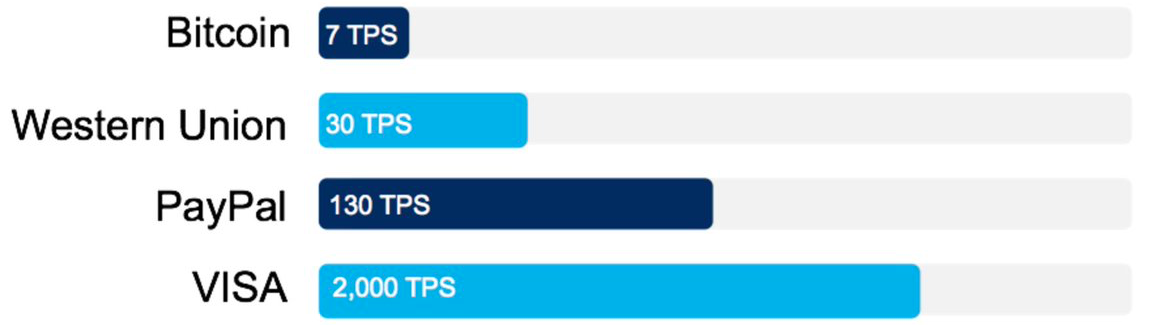
\includegraphics[width = .6\textwidth]{TPS.png}
						\caption{Bitcoin、Western Union\supercite{WesternUnion}、PayPal\supercite{PayPal}以及VISA每秒支持交易量比較圖\supercite{digibyte}}\label{TPS}
					\end{figure}

					\begin{figure}[!htbp]
						\centering
						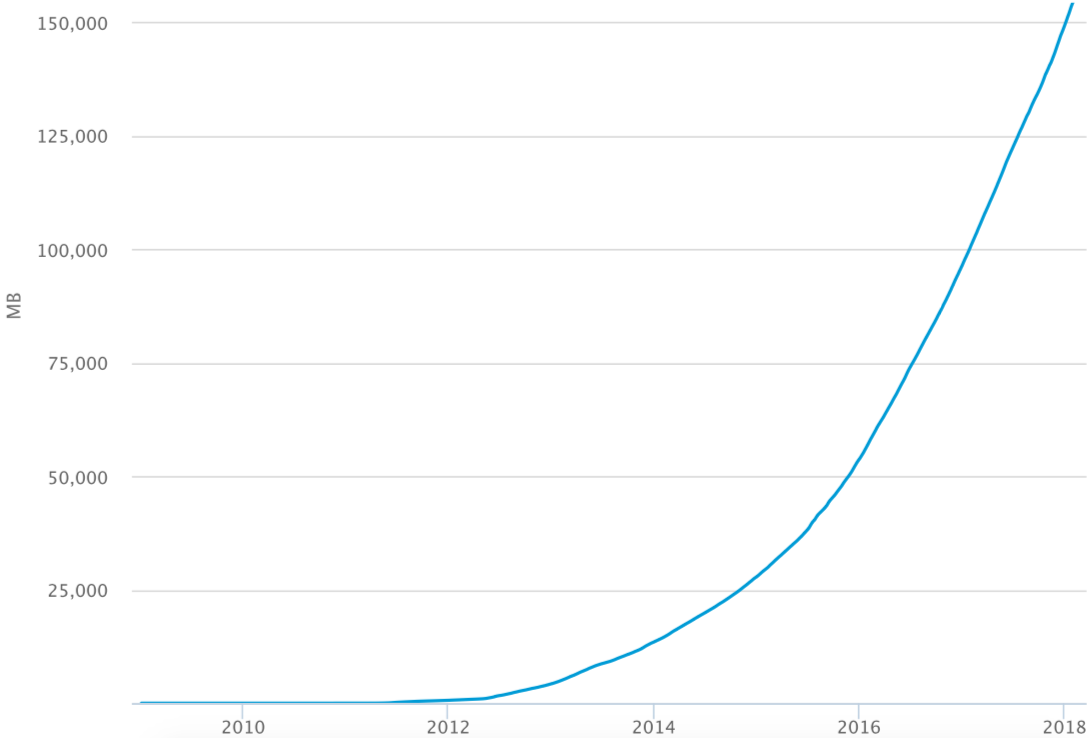
\includegraphics[width = .8\textwidth]{blockchainsize.png}
						\caption{比特幣區塊鏈成長走勢圖\supercite{blockchainsize}}\label{blockchainsize}
					\end{figure}


					\begin{enumerate}
						\item 區塊鏈成⾧速度過快造成節點崩潰。區塊鍊成長速度過快會造成去比特幣全節點不堪負荷:從2009年至今的比特幣區塊鏈大小已達到156GB,這樣的成長速度因為比特幣區塊大小的最大值被設置為1MB。圖\ref{blockchainsize}為過去比特區塊鏈大小,圖中可以發現,於2016年開始,比特幣區塊鏈的成長速度為一直線,這表示著比特幣網絡中持續維持在供不應求的狀況。為解決比特幣每秒⽀持交易量上限的窘迫,現今對⽐特幣的每秒處理交易量有許多優化的⽅案,其中包括解除比特幣區塊大小1MB的限制。在一個區塊上限為1MB的限制下,滿載的比特幣系統中,比特幣區塊鏈平均每十分鐘會增1MB,每小時會增加6MB,每天會增加144MB,每月會增加4.2GB,每年會增加高達50GB,要達到1TB的區塊鏈大小還需要8年,在8年後的未來存儲1TB的數據量應該不會有太大的負擔。倘若解除1MB的區塊限制,在系統的每秒處理交易量看似可以接受更多的交易成倍成長,面臨1TB的比特幣區塊鏈數據會在更短的時間內出現,倘若存儲區塊鏈的成本超過了摩爾定律的成長曲線,會進一步造成使用者自願成為比特幣全節點的意願度降低,使得比特幣網絡的全節點數變少,導致比特幣點對點網絡逐漸轉向中心化網絡發展,失去一開始點對點網絡的意義。

						\item 造成區塊鏈最新區塊同步延遲而使區塊鏈分岔。對於區塊鏈的區塊同步延遲同時也會造成比特幣網絡的影響,J. Göbel於“Increased block size and Bitcoin blockchain dynamics”\supercite{TelecommunicationNetworksandApplicationsConferenceITNAC201727thInternational}有著詳細的研究,在上修區塊大小上限的議題上,使用者因系統占用量提高,⾃願成為⽐特幣全節點意願度下降,此舉可能對⽐特幣點對點網絡建構出的區塊鏈同步上造成延遲,在1055個比特幣全節點當中,平均每十分鐘會有礦工於其中一個全節點生成一個最新的區塊,該最新的區塊會以點對點網絡協議同步到其他1054個節點上。在比特幣系統中,長年來的過程經驗可以發現在礦工生成1MB的區塊後同步到全網節點可以在創造下一個區塊之前完成。倘若將區塊大小修改為2MB或是更大,會使得比特幣全節點的最新區塊同步延遲現象更加明顯,同步延遲會使得區塊鏈分岔,造成1055個比特幣全節點的信息不一致,近一步造成整個比特幣點對點網絡崩潰。
					\end{enumerate}
					

				第二,洗錢防治困難。匿名性為比特幣系統一大特色,比特幣的地址生成的熵是256 bits,亂數是在$2^{256}$的組態空間中隨機選取,這樣的地址與現實生活中的身份並無任何關聯,使得黑市交易、洗錢防治變的困難,甚至有更為前沿的加密貨幣Monero\supercite{noether2014monero}導入了環簽章(Ring Signature)\supercite{Thresholdringsignaturesandapplicationstoad-hocgroups}算法、Zcash\supercite{zhong2002faster}導入零知識證明算法\supercite{Zero-KnowledgeProofsofIdentity},使得原本公開透明的區塊鏈,變得無法檢視,進而造成加密貨幣在洗錢防治上更加的困難。2017年由Thibault de Balthasar and Julio Hernandez-Castro 所提出的論文"An Analysis of Bitcoin Laundry Services."\supercite{AnAnalysisofBitcoinLaundryServices},致⼒探究⽐特幣匿名交易下的資⾦流動模型,試圖以機械學習的方法找出比特幣洗錢模型作為洗錢的工具,圖\ref{Darklaunderworkflow}為該論文針對黑市交易中的洗錢服務運營商Darklaunder進行洗錢機械學習識別有著傑出的成果。

					\begin{figure}[!htbp]
						\centering
						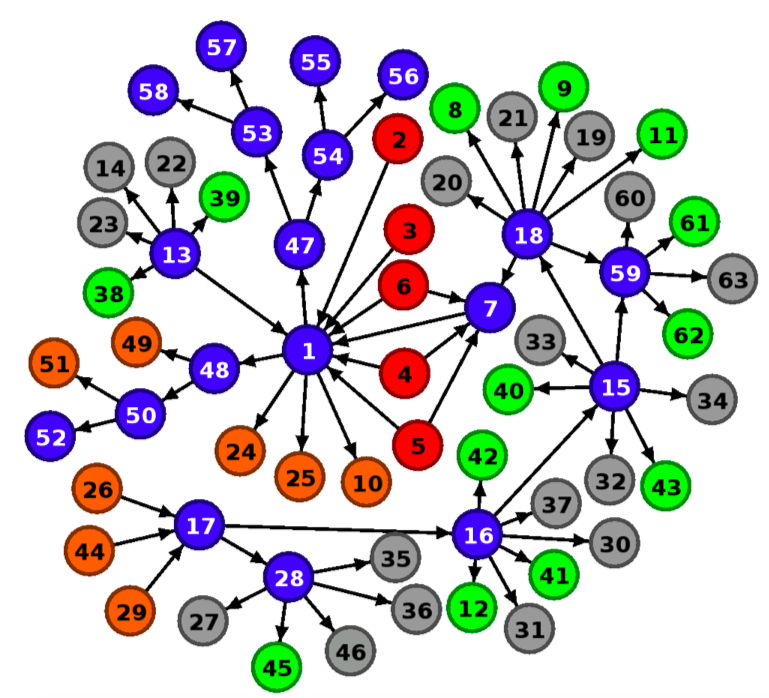
\includegraphics[width = .6\textwidth]{Darklaunderworkflow.png}
						\caption{Darklaunder 洗錢模型\supercite{AnAnalysisofBitcoinLaundryServices}}\label{Darklaunderworkflow}
					\end{figure}

				第三,低可擴展性。區塊鏈架構為了防止各式的攻擊,所以在架構訂定以及接口設計都有著嚴謹的規範。以下將闡述造成比特幣低可擴展性的原因:

					\begin{enumerate}

						\item 修改比特幣協議製作添加外部信息的區塊鏈:比特幣區塊鏈技術是一個嚴謹的架構,倘若要創造可以支持外部信息的結構需要重新創造全新的加密貨幣,大部分的加密貨幣不支持外部輸入,由於外部的信息輸⼊無法保證其信息的正確性,近一步造成垃圾進垃圾出(Garbage In, Garbage Out,GIGO)的問題,倘若錯誤的信息存儲在無法刪除、修改的區塊鏈下,只是強化該筆錯誤信息的錯誤。如食品履歷區塊鏈,致力於將食品生產到超市的過程逐一記錄在區塊鏈上,但如果一開始在輸入信息時,無法保證其信息之正確性,則該食品履歷區塊鏈則毫無意義,錯誤的信息內容甚至可能使該錯誤被強化。

						\item 於區塊頭或交易信息添加外部信息:比特幣區塊鏈上,可以添加一些信息於區塊上,該信息會永久保存於區塊鏈上,除了在區塊上新增信息,在比特幣單筆交易信息上,亦可填寫一些私人信息,但這樣的空間大小有限,且現今的比特幣價格日趨上漲,比特幣交易手續費是以單筆交易大小計算,這將使得在交易中添加些個人信息變得更加昂貴。

					\end{enumerate}

				在比特幣系統中,其區塊鏈僅用於記錄交易記錄,不能擴展更多功能和應用程序。有很多開發者希望將比特幣系統擴展到智能合約等其他應用程序。但是,後來發現改變原始比特幣系統框架是具有挑戰性的工作。因此,全球第二大加密貨幣以太坊(Ethereum,ETH)的作者Vitalik選擇了創建了以太坊虛擬機(Ethereum Virtual Machine,EVM),而非改變原始的比特幣系統框架。以太坊虛擬機所創建的智能合約可以在統一的以太坊平臺上運行,而以太坊也藉此突破了比特幣之技術瓶頸。
	
	\subsection{國際情勢分析}
	\begin{table}[!htbp]
		\centering
		\caption{各國政府對比特幣態度統整表}
		\label{world}
		\begin{tabular}{@{}|l|l|c|c|l|@{}}
		\toprule
		\multicolumn{1}{|c|}{\multirow{2}{*}{序號}} & \multicolumn{1}{c|}{\multirow{2}{*}{國家}} & \multicolumn{2}{c|}{接納} & \multicolumn{1}{c|}{\multirow{2}{*}{禁止}} \\ \cmidrule(lr){3-4}
		\multicolumn{1}{|c|}{} & \multicolumn{1}{c|}{} & 歡迎/放任 & 監管 & \multicolumn{1}{c|}{} \\ \midrule
		1 & 伊朗 & \begin{tabular}[c]{@{}c@{}}監管得當歡迎\\ 比特幣發展\end{tabular} &  &  \\ \midrule
		2 & 以色列 & \begin{tabular}[c]{@{}c@{}}歡迎:欲發展\\ 國際ICO中心\end{tabular} &  &  \\ \midrule
		3 & 法國 & \begin{tabular}[c]{@{}c@{}}放任:與實體\\ 經濟無關\end{tabular} &  &  \\ \midrule
		4 & 美國 & 暫不構成威脅 &  &  \\ \midrule
		5 & 新加坡 & \begin{tabular}[c]{@{}c@{}}不監管但注意\\ 周邊活動\end{tabular} &  &  \\ \midrule
		6 & \begin{tabular}[c]{@{}l@{}}沙特阿拉\\ 伯王国\end{tabular} & \begin{tabular}[c]{@{}c@{}}加密貨幣尚未\\ 成熟,不監管\end{tabular} &  &  \\ \midrule
		7 & 烏克蘭 & 不屬於貨幣 &  &  \\ \midrule
		8 & 韓國 &  & \begin{tabular}[c]{@{}c@{}}很快將監管\\ 交易所\end{tabular} &  \\ \midrule
		9 & 菲律賓 &  & 計劃監管ICO &  \\ \midrule
		10 & 英國 &  & 考慮監管 &  \\ \midrule
		11 & 馬來西亞 & \multicolumn{1}{l|}{} & 正規化監管框架 & \multicolumn{1}{c|}{} \\ \midrule
		12 & 俄羅斯 & \multicolumn{1}{l|}{} & \begin{tabular}[c]{@{}c@{}}2018年7月前\\ 完成立法\end{tabular} & \multicolumn{1}{c|}{} \\ \midrule
		13 & 日本 & \multicolumn{1}{l|}{} & \begin{tabular}[c]{@{}c@{}}任命加密貨幣\\ 監察長\end{tabular} & \multicolumn{1}{c|}{} \\ \midrule
		14 & 香港 & \multicolumn{1}{l|}{} & ICO須受法規監管 & \multicolumn{1}{c|}{} \\ \midrule
		15 & 辛巴威 & \multicolumn{1}{l|}{} &  & \multicolumn{1}{c|}{定法前,屬非法} \\ \midrule
		16 & 摩洛哥 & \multicolumn{1}{l|}{} &  & \multicolumn{1}{c|}{禁止加密貨幣交易} \\ \midrule
		17 & 印尼 & \multicolumn{1}{l|}{} &  & \multicolumn{1}{c|}{\begin{tabular}[c]{@{}c@{}}2018年前\\ 全面禁止\end{tabular}} \\ \midrule
		18 & 中國 & \multicolumn{1}{l|}{} &  & \multicolumn{1}{c|}{禁止加密貨幣} \\ \bottomrule
		\end{tabular}
		\end{table}
	
	比特幣是一種全新的價值交換的媒介,因為區塊鏈技術相當新穎,在各個國家所秉持的態度皆有所不同,大致可將個國家對比特幣的政策分為兩大類,分別為接納與禁止;在接納加密貨幣的分類當中又分為歡迎、放任以及監管。

	在歡迎、放任的政策下的國家包括伊朗、以色列、法國、美國、沙特阿拉伯王國、烏克蘭以及新加坡,上述國家政策上皆已抱持著開放且不監管的方式接納加密貨幣,這些國家認為加密貨幣對於國家金融科技的發展具有前景;在分類於接納但是實施監管的國家中,包括韓國、菲律賓、英國、馬來西亞、俄羅斯、日本以及香港地區皆認為加密貨幣技術可能存在的高風險,且針對加密貨幣的洗錢防制以及非法集資進行嚴格管理,也進一步制定相關的法律,使得國家可以應對新型加密貨幣的糾紛;在禁止加密貨幣的分類中包括辛巴威、摩洛哥、印尼以及中國,這些國家認為比特幣是一個非法的貨幣,因為涉及到洗錢問題、難以實施外匯管制。但是對於區塊鏈技術層面上之探討,在所有國家中都是以蓬勃發展的正面態度看待。上述各國政府對⽐特幣態度如表\ref{world}:

		

	\section{研究目標與內容}
	比特幣在各個國家的蓬勃發展且應用在相當多的領域,應用的領域包括交易所、去中心化交易所、兌幣所、遊戲點數、網路購物、資產的保存、募資以及遠距離支付,甚至是各國的銀行和金融機構都逐步投入人力及資金研究區塊鏈相關技術,甚至是訂定各國相關的法律。在比特幣資產的流動上存在著許多的問題,第一,比特幣的帳戶是由亂數產生器生成,該比特幣帳戶與在現實生活中的使用者並無直接關聯,使得比特幣洗錢變更加盛行。第二,現今的比特幣交易皆為匿名對匿名支付,並無正式的收據開立,使得消費者在購物後,倘若商品存在問題,無法得到法律上的保障。第三,因為比特幣是匿名支付給匿名的交易,使得政府無法從交易行為中進一步課徵稅收,滯礙國家經濟發展。

	本文將解決上述三項問題,設計與實現一個比特幣的實時交易實時监督系统達到下列幾點目標:

		\begin{enumerate}
			\item 導入匿名顧客支付給實名商家的交易模型到加密貨幣交易系統。
			\item 設計與實現在加密貨幣交易中匿名顧客支付給實名商家的交易監督系統;
			\item 於政府端導入多重簽章算法,使比特幣的实时交易监督系统比透過 Green Address 機構驗證更加快速。
			\item 利用多重簽章算法的機制可以讓商家預防比特幣雙重支付的攻擊。
			\item 商家和商品信息管理⼦系統讓商家可進行庫存管理及商家商品管理。
			\item 實現於加密貨幣交易中,消費者匿保持匿名同時也保障消費者權益。
			\item 透過對商家進行實名制,比特幣的交易監督系統讓政府主管機關可以有效獲得稅收。
		\end{enumerate}

	為實現上述目標,本文首先將詳細探討區塊鏈技術的優勢,藉由深度了解區塊鏈技術的優勢可以取之優點,如區塊鏈是一個不間斷、不可竄改、去中心化、公開數據庫、穩定的系統。第二,探討區塊鏈技術的劣勢,區塊鏈技術並非完美,存在著洗錢、逃漏稅、無法保障消費者權益以及交易速度慢的問題,藉由瞭解問題,並設計系統解決。第三,交易模型分析,透過交易模型分析探討在現金、電子貨幣以及加密貨幣存在的交易模型,並在諸多交易模型中發現,匿名支付給實名的交易行為,可以保障消費者隱私,同時保障消費者權益,更使得政府可以對商家的營收進行檢視。第四,系統設計,完成交易分析,並著⼿設計數據庫模型。第五,系統詳細設計與實現,利⽤Java 編程語⾔實現主系統以及三個⼦系統。第六,系統優化,引入比特幣的多重簽章算法,實現比特幣的實時交易監督系統。第七,功能測試,測試以Java編寫程序所有的功能是否能夠完整運作。第八,性能測試,測試在未進行優化的系統與已經優化的系統兩者之間效能的差異。


	\section{論文組織結構}
	在本節中將逐一說明本論文的組織結構共分為七章,分別為緒論、相關理論與技術、系統需求分析、系統概要設計、系統實現、系統測試以及总结与展望:

	第一章:簡述區塊鏈技術解決現有數據庫存在的信息不一致、信息安全問題以及數據庫損毀問題
	。說明在加密貨幣市場中不僅只是比特幣,亦有許多新穎技術為特色的貨幣競爭。簡要探討區塊鏈技術的優點,逐一探討比特幣的缺點及區塊鏈技術瓶頸。最後於研究目標與內容當中,闡述本文的待解決問題以及解決方法。

	第二章:介紹比特幣的發展,闡述比特幣地址生成運用到的算法、生成過程以及多重簽章算法。並詳細說明區塊鏈結構及所有欄位變數與區塊鏈相關的意義。

	第三章:首先對五種交易模型進行分析,進而得知匿名對實名的交易,既可以保障消費隱私且兼具保有消費者權益,並透過需求分析探討本系統需構建的功能模塊。

	第四章:概要設計比特幣交易监督系统的架構,以及說明三個子系統的模塊功能。設計本系統的數據庫結構,設計ER實體聯繫模型 (Entity-relationship model),並闡述本系統的運作流程。最後則將多重簽章算法引入本系統,使得本系統成為比特幣的實時交易监督系统。

	第五章:詳細設計商家和商品信息管理子系統、商家移動裝置收款及交易子系統以及客戶端移動支付和交易子系統的介面。

	第六章:透過功能測試逐一檢視所有功能是否能夠正常運行,經由性能測試分析原始系統與優化後的系統效能之間的差異。

	第七章:說明比特幣區塊鏈系統透過本文所提出之系統,可以達到保障消費者權益同時也兼顧保有顧客隱私,也使得政府可以透過該系統檢視交易明細課徵稅收,而商家亦可對庫存及產品進行管理,達到三贏的局面。

	% Copyright (c) 2014,2016 Casper Ti. Vector
% Public domain.

\chapter{文獻探討}

	\section{比特幣(Bitcoin)}
	比特幣(Bitcoin,BTC)是一個點對點式的電子現金系統,集成了非對稱式金鑰密碼學(Asymmetric Key Cryptography)\supercite{AsymmetricKeyCryptography}、簽章密碼學(Signature cryptography)、零知識證明密碼學(Zero Knowledge Proof Cryptography)\supercite{Zero-KnowledgeProofsofIdentity}、哈希函數密碼學(Hash function cryptography)、共式算法(Consensus)諸多技術建構了一個分散式、不需要仰賴中心化機構加以維護的交易帳本(區塊鏈)。在接下來的章節中將逐一進行詳盡的說明每個技術在各個環節中所扮演的角色。

	\section{比特幣地址(Bitcoin Address)}
	⽐特幣地址為⽐特幣的載體,深⼊了解⽐特幣的地址⽣成相關算法、⽐特幣地址⽣成過程、多重簽名,可以近⼀步應⽤在区块链的实名交易监督系统。

		\subsection{比特幣地址生成相關算法}
		在點對點的現金系統中,首先必須先生成一個地址,在比特幣的協議中有著既定的程序生成地址。運用到的技術包括亂數產生器、secp256k1\supercite{johnson2001elliptic}、SHA-256(哈希函數)\supercite{DBLP:conf/fse/KhovratovichRS12}、RIPEMD-160(哈希函數)\supercite{DBLP:conf/isw/MendelPRR06}、Base58\supercite{Base58}。接下來將詳述每一個函數的運作過程以及意義,最後說明比特幣交易地址生成的每一個步驟。
		
			\subsubsection{亂數產生器(Random number generator)}
			亂數在密碼學中是個相當重要的一環,在比特幣系統中更是重要,畢竟生成的亂數會變成比特幣的私鑰,私鑰是簽署資產轉移的唯一方式,在比特幣地址中的亂數產生器會產出一個256 bits長度的亂數,也就是私鑰,256 bits的長度可以表現的組態空間為$2^{256}$,換算成十進位表示為$1.1579209x10^{77}$,要在這組態空間中,以亂數產生同樣的一把私鑰是一件困難的事,但也有國際的實驗室\supercite{TheLargeBitcoinCollider}團隊正在努力的窮舉比特幣$2^{256}$的組態空間,如圖\ref{LBC}所示,根據LBC公布的數據顯示,目前已經完成了$2.330109x10^{16}$個地址探索。雖然$10^{16}$的級別與$10^{77}$的級別相距甚遠,但LBC已探索的組態空間中擊中了15個比特幣地址,團隊也將這15個地址的1.180899個比特幣轉走。

			\begin{figure}[h]
				\centering
				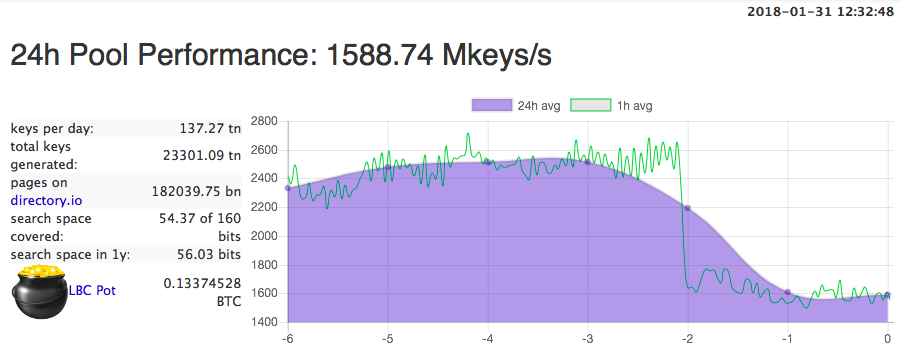
\includegraphics[width = .9\textwidth]{LBC.png}
				\caption{LBC窮舉比特幣私鑰算力狀態圖\supercite{TheLargeBitcoinCollider}}\label{LBC}
			\end{figure}

			如何建構一個亂數,在過往的亂數產生器往往會加入時間作為參數,但對於一個攻擊者而言,只需要去猜測在這段時間內目標者所有生成的可能性有極高的機率可猜出亂數。而亂數在密碼學中常會是一把私鑰的生成,在https協議中,服務器端與客戶端,建立一個加密連線的過程中也需要一個亂數去建立一個高安全性的加密通道-傳輸層安全性協定(Transport Layer Security,TLS)\supercite{dierks2008transport},在SSH協議中也採用了亂數。
	
			在過去的歷史事件中,發現Android手機版以及平板版的亂數產生器中存在著不隨機,於2013年8月比特幣開發者Mike Hearn提及“All private keys generated on Android phones/tablets are weak and some signatures have been observed to have colliding R values” \supercite{SomeSecureRandomThoughts},Bitcoin.org也發布了警告\supercite{AndroidSecurityVulnerability}簡要說明該事件的原因,以及表明影響到的Bitcoin Wallet 客戶端有Bitcoin Wallet、BitcoinSpinner、Mycelium Bitcoin Wallet、blockchain.info。這樣的錯誤源於Android本身支持的亂數產生器並不隨機,隨後Android解釋了亂數的問題並加以修正。在這Android手機亂數不夠亂的事件中,有自願者自發性地公布自己的損失狀態,總金額為55.82152538個比特幣\supercite{Badsignaturesleading},但因為比特幣屬於被動的性質,無人主動回報即不會加入統計中,所以總損失估計會超過55.82152538個比特幣。

			\subsubsection{Secp256k1}
			在密碼學中有分對稱式加密與非對稱式加密,對稱式加密又分為信息流加密與信息塊加密,信息流加密著名的是由美國密碼學家Ron Rivest教授設計,包括RC2(1987年)\supercite{OnthedesignandsecurityofRC2}、RC4(1987年)\supercite{Rc4}、RC5(1994年)\supercite{TheRC5encryptionalgorithm}、RC6(1998年)\supercite{TheRC6blockcipher.v1.1August201998};信息塊加密著名的有数据加密标准(Data Encryption Standard,DES,1975年)\supercite{Dataencryptionstandard}、三重数据加密算法(Triple Data Encryption Algorithm,Triple DES,1998年)\supercite{TrippleDataEncryptionAlgorithmModesofOperation}、高级加密标准(Advanced Encryption Standard,AES,1998年)\supercite{ThedesignofRijndael:AES-theadvancedencryptionstandard};非對稱式加密最廣為人知的有RSA(Rivest–Shamir–Adleman,1977年)\supercite{Cryptographiccommunicationssystemandmethod}、椭圆曲线密码学(Elliptic curve cryptography,ECC,1985年)\supercite{Ellipticcurvecryptosystems}。
			非對稱式加密與對稱式加密最大的不同在於,對稱式加密在加密解密的過程中只需要一把鑰匙,而非對稱式加密會生成兩把鑰匙分別為私鑰與公鑰,在算法的設計上一開始會以亂數產生一把私鑰,再經由非對稱式加密算法推導出公鑰,推導出的公鑰在非對稱式密碼學中並無直接的方法可以反推至私鑰,如此一來確立私鑰的安全性。非對稱式密碼的使用場景有兩種,第一種是希望收到加密信息的Alice,Alice會生成私鑰存儲在自己本地端的電腦中,並將推導出的公鑰公布在网络上,這時希望聯繫Alice的Bob在网络上取得公鑰後,Bob會以Alice的公鑰進行加密,之後將密文寄送給Alice,在傳遞信息的過程中,既使网络存在著監聽,也無法將信息順利解密,唯有Alice收到信息後使用Alice原本產生該公鑰的私鑰,才可以解出明文。第二種則應用在比特幣的交易之數字簽名以及交易驗證交易,比特幣地址的創建過程中會透過secp256k1生成私鑰公鑰對,在創建比特幣交易的過程中,使用該地址的私鑰對該地址未花费的输出(Unspent Transaction Output,UTXO)進行數字簽名,完成數字簽名後會與公鑰以及交易信息一起廣播到比特幣网络的交易緩池持當中,比特幣交易緩存池存在於所有比特幣全節點當中,主要存儲所有未被收入到比特幣區塊鏈內的所有交易,也就是零確認交易,等待礦工將該筆交易收入至比特幣區塊鏈當中。
			比特幣採用的secp256k1是屬於椭圆曲线密码学中的一個版本,不同的橢圓曲線版本的差異在於不同的初始參數,包括橢圓曲線方程$$y^2=x^3+ax+b$$、$p$=FFFFFFFFFFFFFFFFFFFFFFFFFFFFFFFFFFFFFFFFFFFFFFFFFFFFFFFEFFFFFC2F為巨大的素數、G點被称为⽣成点的常数点亦稱為基點。至於為什麼選擇ECC而非RSA的主要原因,其一在於ECC在生成密鑰對所需的時間更佳快速,圖\ref{ECCtime}為Nicholas Jansma於2004年針對ECC與RSA的密鑰對生成時間與數字簽名所需時間的論文\supercite{Performancecomparisonofellipticcurveandrsadigitalsignatures}顯示,當ECC產生571 bits的密鑰長度,RSA要達到相同的安全性需要生成15360 bits,這也導致生成時間產生高達471倍之差距。
			
			\begin{figure}[h]
				\centering
				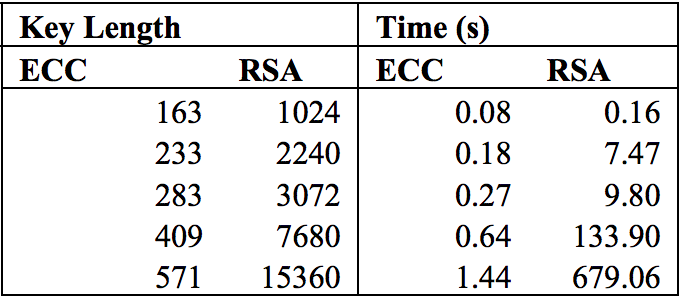
\includegraphics[width = .5\textwidth]{ECCtime.png}
				\caption{ECC與RSA的密鑰對生成時間比較圖\supercite{Performancecomparisonofellipticcurveandrsadigitalsignatures}}\label{ECCtime}
			\end{figure}

			除了在密鑰對生成時間ECC有著比RSA更高效的算法外,在安全性上ECC可以更短的密鑰長度達到與RSA相同的安全強度,L Ducas針對ECC、RSA、BLISS做出了深度的安全性探討\supercite{LatticesignaturesandbimodalGaussians},圖\ref{LatticesignaturesandbimodalGaussians}同樣達到80 bits的安全性級數,RSA 1024需要1024 bits,ECDSA 160僅需要160 bits,該篇論文除了探討RSA與ECDSA之外,更大的部分在闡述量子計算機對於既有的傳統密碼帶來的抨擊,有機會快速窮舉$2^{256}$的比特幣私鑰,在未來量子計算機的蓬勃發展擁有2000 qbits運算能力,量子計算機可以快速窮舉破解所有的比特幣私鑰。因此發展針對量子計算機設計的數字簽名算法成為密碼學上嶄新的議題,而BLISS則為針對量子計算機所設計的抗量子計算的簽名算法。

			\begin{figure}[h]
				\centering
				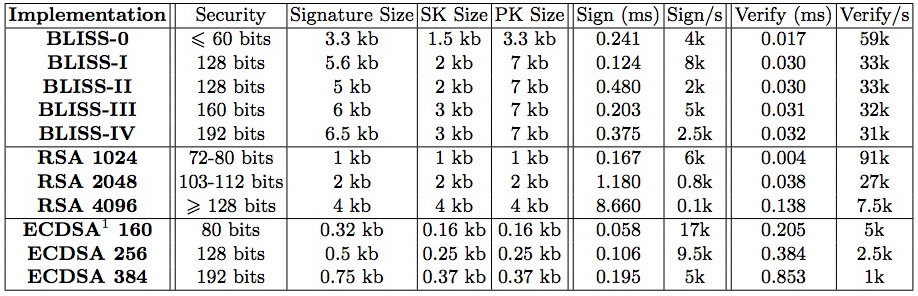
\includegraphics[width = 1\textwidth]{LatticesignaturesandbimodalGaussians.png}
				\caption{算法BLISS、RSA、ECDSA安全級數比較圖\supercite{LatticesignaturesandbimodalGaussians}}\label{LatticesignaturesandbimodalGaussians}
			\end{figure}

			\subsubsection{SHA-256}
			哈希下數在比特幣系統中扮演著相當多的角色,包括比特幣地址生成、比特幣交易哈希指針、比特幣區塊哈希指針、比特幣挖礦算法工作量證明。哈希算法有幾大特色,分別為
			\subsubsection{RIPEMD-160}
			\subsubsection{Base58}

		\subsection{比特幣地址生成過程}

		\begin{figure}[h]
				\centering
				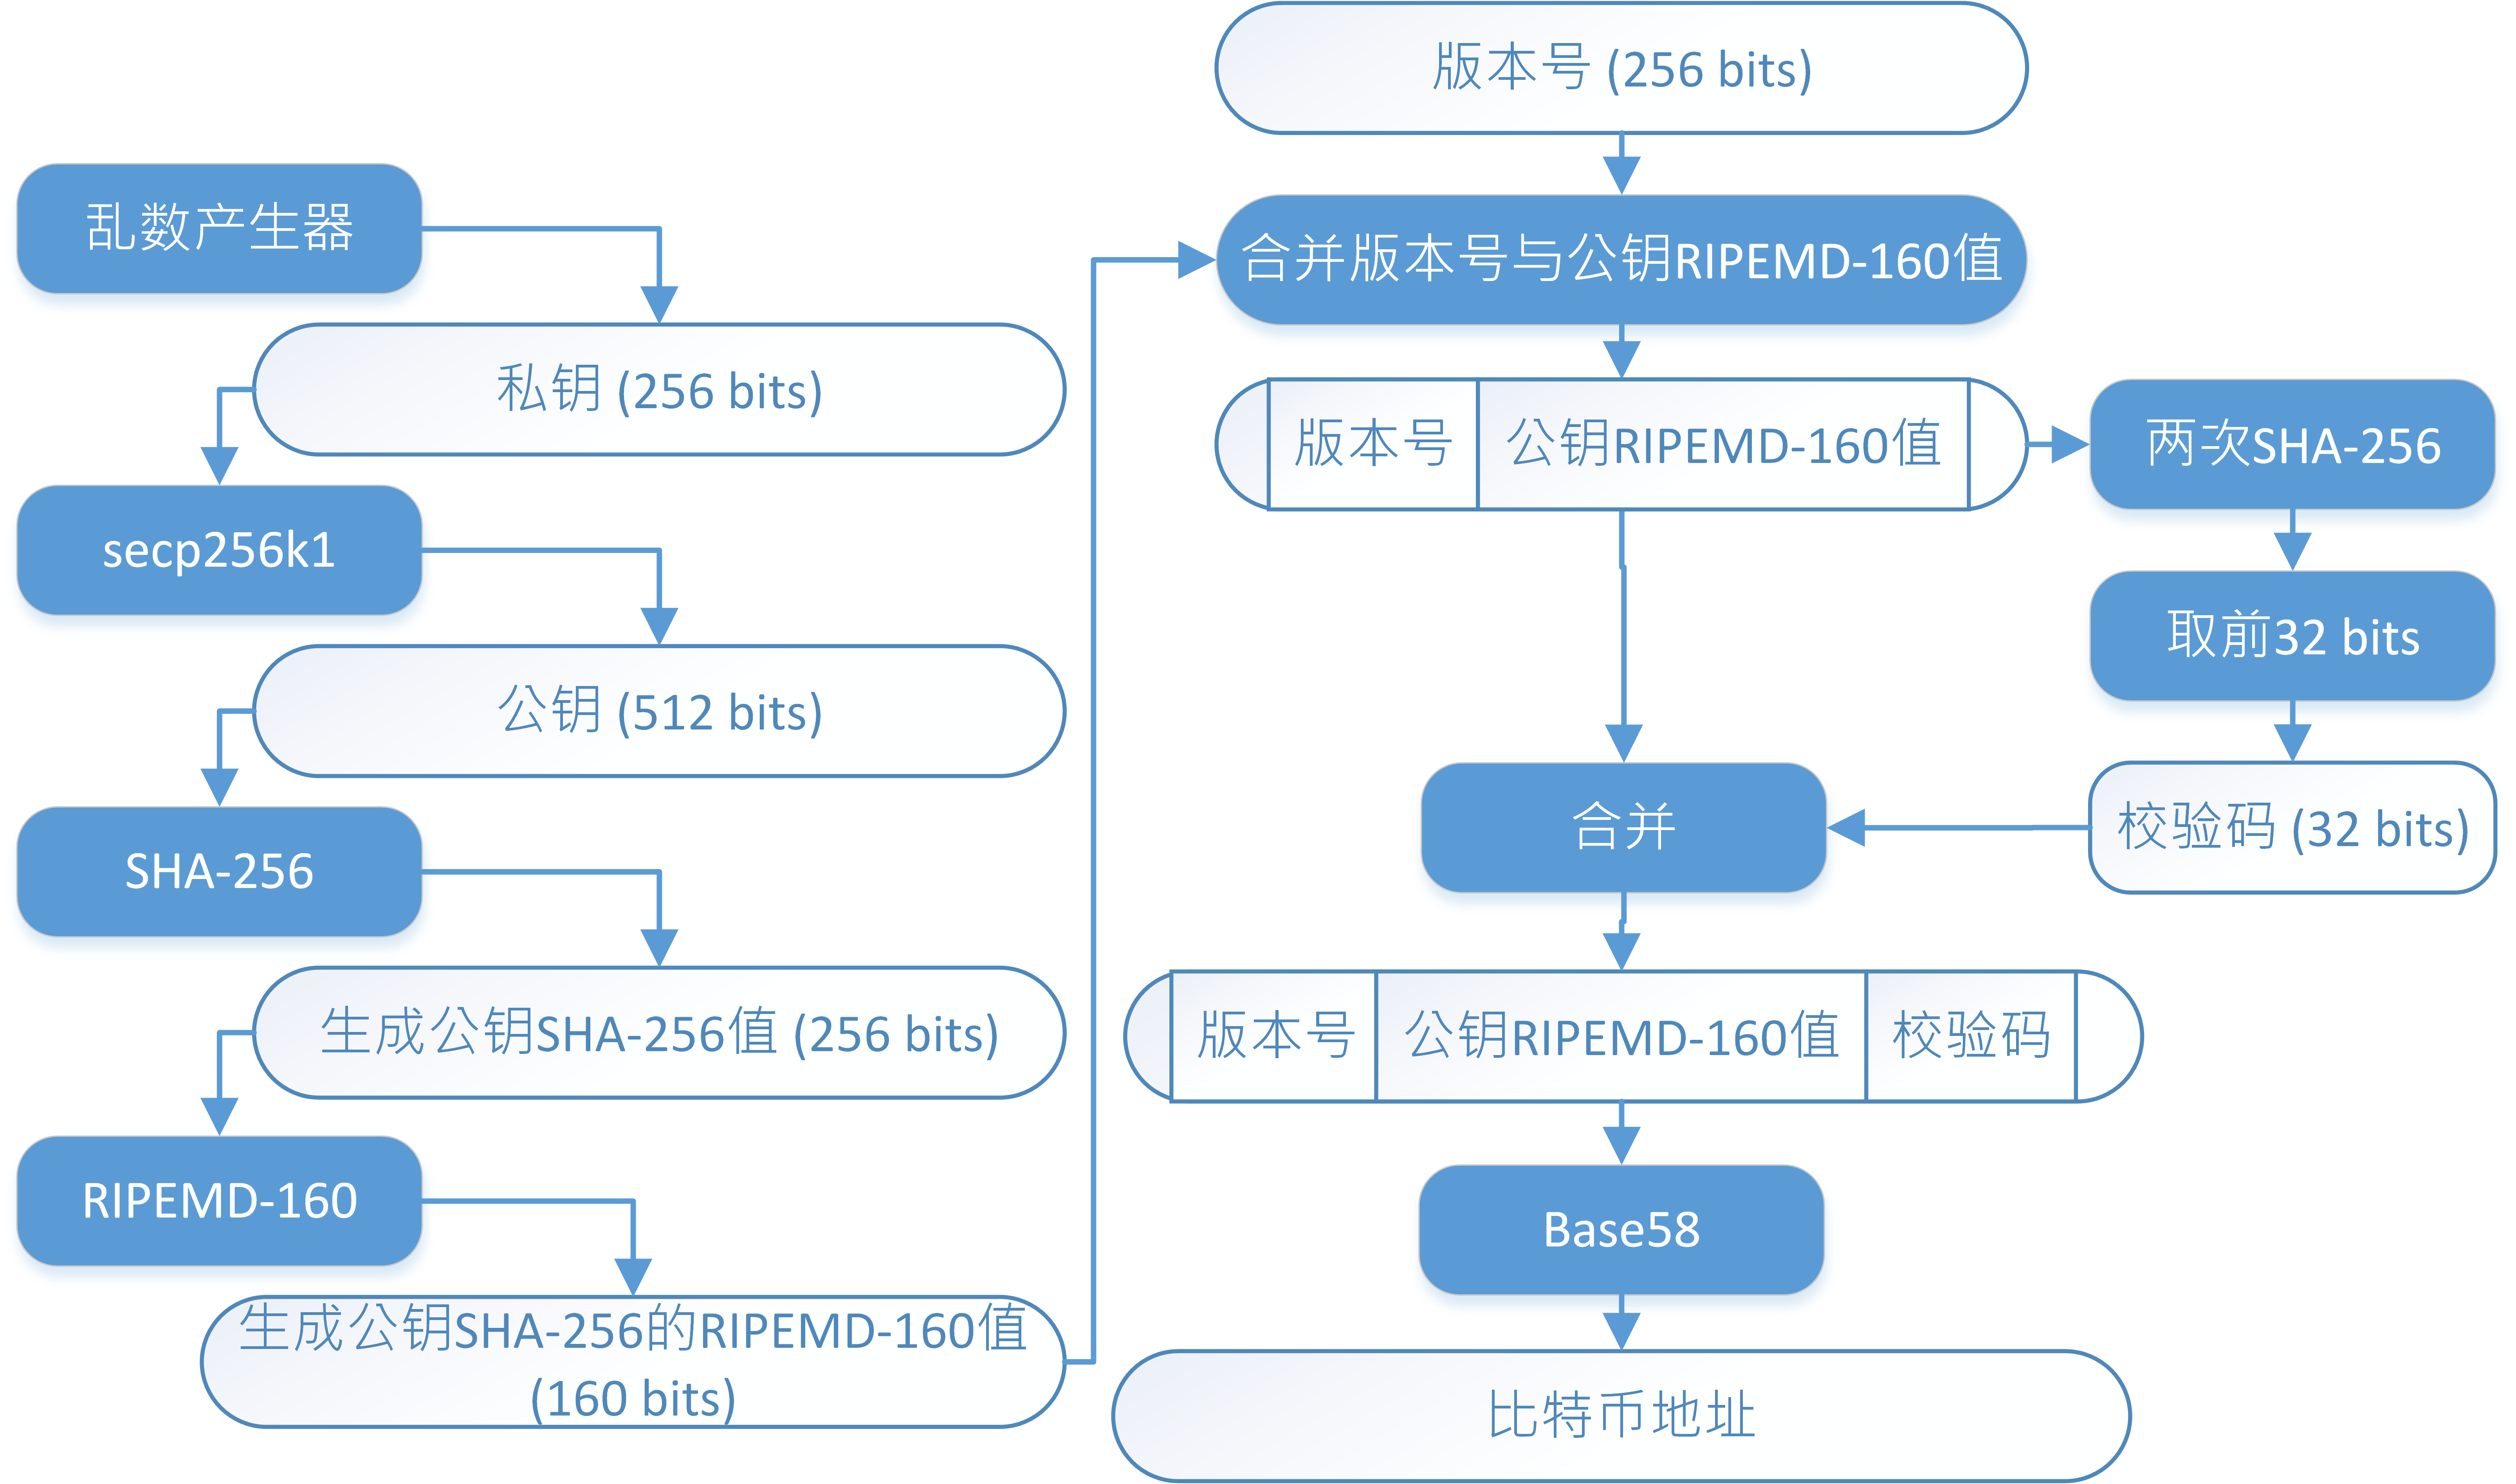
\includegraphics[width = .9\textwidth]{address.png}
				\caption{比特幣地址生成流程圖}\label{address}
		\end{figure}

		\begin{enumerate}
			\item 生成私鑰:使用亂數產生器產生一個長度在256 bits以內的隨機數,而此隨機數即成為該地址的私鑰,在比特幣系統中,可以利用私鑰(Private Key)簽署花費該地址當中的比特幣。
			\item 生成公鑰:該演算法為一個以橢圓曲線演算法為基礎的一個標準,而不同標準的差異在於初始化的參數,這些參數的訂定皆經過嚴謹的考核及實驗測試。在比特幣系統中該算法扮演著私鑰轉換為公鑰的角色。這使得比特幣交易使用私鑰進行簽署之後,還可以使用公鑰校驗該筆交易的正確性。
			\item 生成公鑰SHA-256:一種哈希函數,哈希函數的特性有許多,包括雪崩效應、不可預測、不可逆、校驗檔案是否完整。在此步驟中是將公鑰帶入SHA-256 函數中,產出長度為256 bits的哈希值。
			\item 生成公鑰SHA-256的RIPEMD-160:亦為哈希函數的一種,特色符合哈希函數的特性,與SHA-256不同的是RIPEMD-160產出的長度為160 bits。
			\item 取得版本號:比特幣在一開始設計的過程中,便定義了不同的地址樣式及功能,在第五個步驟中會加入版本號加以區分不同的地址。
			\item 校驗碼生成:校驗碼為比特幣地址生成過程中重要的一環,可在支付比特幣的過程中降低因為手誤而將比特幣轉入到不存在(不符合比特幣地址生成規則)地址的可能性。對公鑰SHA-256的RIPEMD-160再做兩次SHA-256,取該哈希值前32 bits的值作為校驗碼。
			\item 版本號、公鑰SHA-256的RIPEMD-160和校驗碼合併:版本號、第四個步驟的產生之公鑰RIPEMD-160及第五個步驟產生之校驗碼合併。
			\item 合併的結果以Base58編碼:將第六步驟組進行合併組合的結果,利用Base58進行編碼,Base58修改自Base64,其與Base64最大不同之處在於移除了"0"、"O"、"I"、"l"、"+"、"/"的字符,可以降低人工判讀在地址的錯誤率。
		\end{enumerate}

		\subsection{多重簽名(Multi-Signature)}
		% 	\subsubsection{多重簽名地址}
		 	\subsubsection{Green Address}
		 	雙重支付問題存在於比特幣交易在未被區塊鏈確認收入到區塊鏈之前,都有機會受到惡意的攻擊者雙重支付(Double-spending)\supercite{Informationpropagationinthebitcoinnetwork}同一筆款項。現今的比特幣區塊產出速度為十分鐘一塊,即便附上足夠的手續費也須等待將近十分鐘的時間,倘若是在手續費不足的情況下,該筆比特幣交易甚至會在比特幣交易緩存池中滯留一週的時間。在手續費足夠的情況下,十分鐘的確認時間會對實體店面的小額交易處理非常的不友善,為了在既有的比特幣區塊鏈的框架底下能夠提升交易速度,因此Green Address技術致力於在一開始創建交易的同時管控雙重支付交易的發生,他們採用了2-of-2多重簽章,也就是創建一個特殊的比特幣地址,這個比特幣地址的持有人有兩個代表人,分別為使用者與Green Address機構節點,這筆交易的建立必須要雙方同時簽署交易才被允許廣播至比特幣网络中。若是遇到交易塞車,且節點緩存池空間不足的問題時,比特幣節點會優先遺棄手續費最低的交易,視同此機交易不曾存在過,故若真的遇到交易被遺棄的情況,Green Address機構節點也會透內部的數據庫紀錄再次廣播此筆交易,並確保此筆交易可以被收入至區塊內。Green Address機構節點也就成為了交易創建的把關者,過濾所有的雙重支付攻擊的發生,也避免交易因為比特幣网络塞車而交易被礦工遺棄的情形。
		 	在這樣的機制下,只要是用Green Address錢包交易即可確認雙重支付攻擊是不會發生的,對商家或是收款人而言,可以得到在即時交易中不被雙重支付攻擊的保障,提升在未進入區塊鏈的交易可確定性,進而創造出即時交易的可行性。

		 	\paragraph{Green Address錢包生成過程}
		 	此節將詳細闡述Green Address錢包生成過程的重要步驟,如圖\ref{gabuild}所示。
		 	\begin{figure}[h]
				\centering
				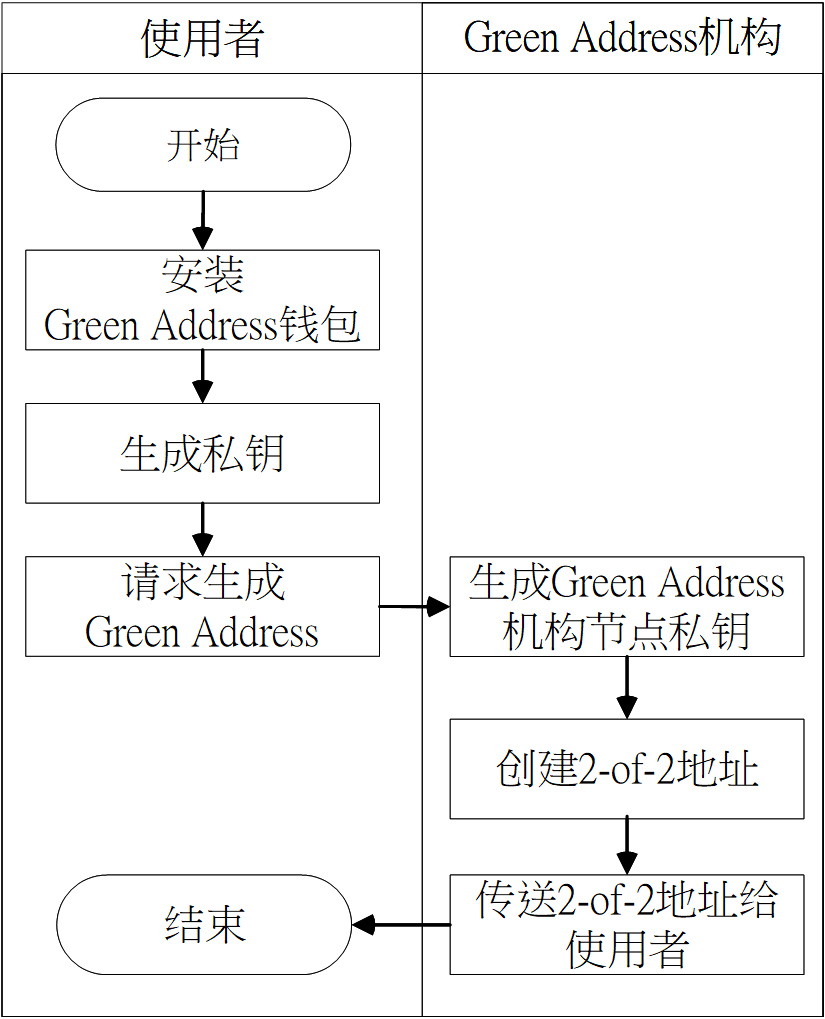
\includegraphics[width = .5\textwidth]{gabuild.png}
				\caption{Green Address錢包生成流程圖}\label{gabuild}
			\end{figure}

		 	\begin{enumerate}
		 		\item 使用者安裝Green Address比特幣錢包,並向Green Address機構節點請求創建2-of-2多重簽章比特幣地址。
		 		\item 使用者與Green Address機構節點分別生成兩把私鑰,共同創建Green Address比特幣地址。
		 		\item 當交易發起時,使用者使用自己的私鑰簽署該筆交易。
		 		\item 將該筆交易傳送到Green Address機構節點。
		 		\item Green Address機構節點收到後,檢查該筆交易是否存在雙重支付攻擊。
		 		\item 確認無攻擊跡象後便廣播至比特幣网络中。
		 	\end{enumerate}

		 	\paragraph{Green Address交易發起流程}
		 	說明完Green Address地址是如何創建之後,該節將詳細說明如何運用多重簽章地址發起交易至比特幣网络中,如圖\ref{gatx}所示。

		 	\begin{figure}[h]
				\centering
				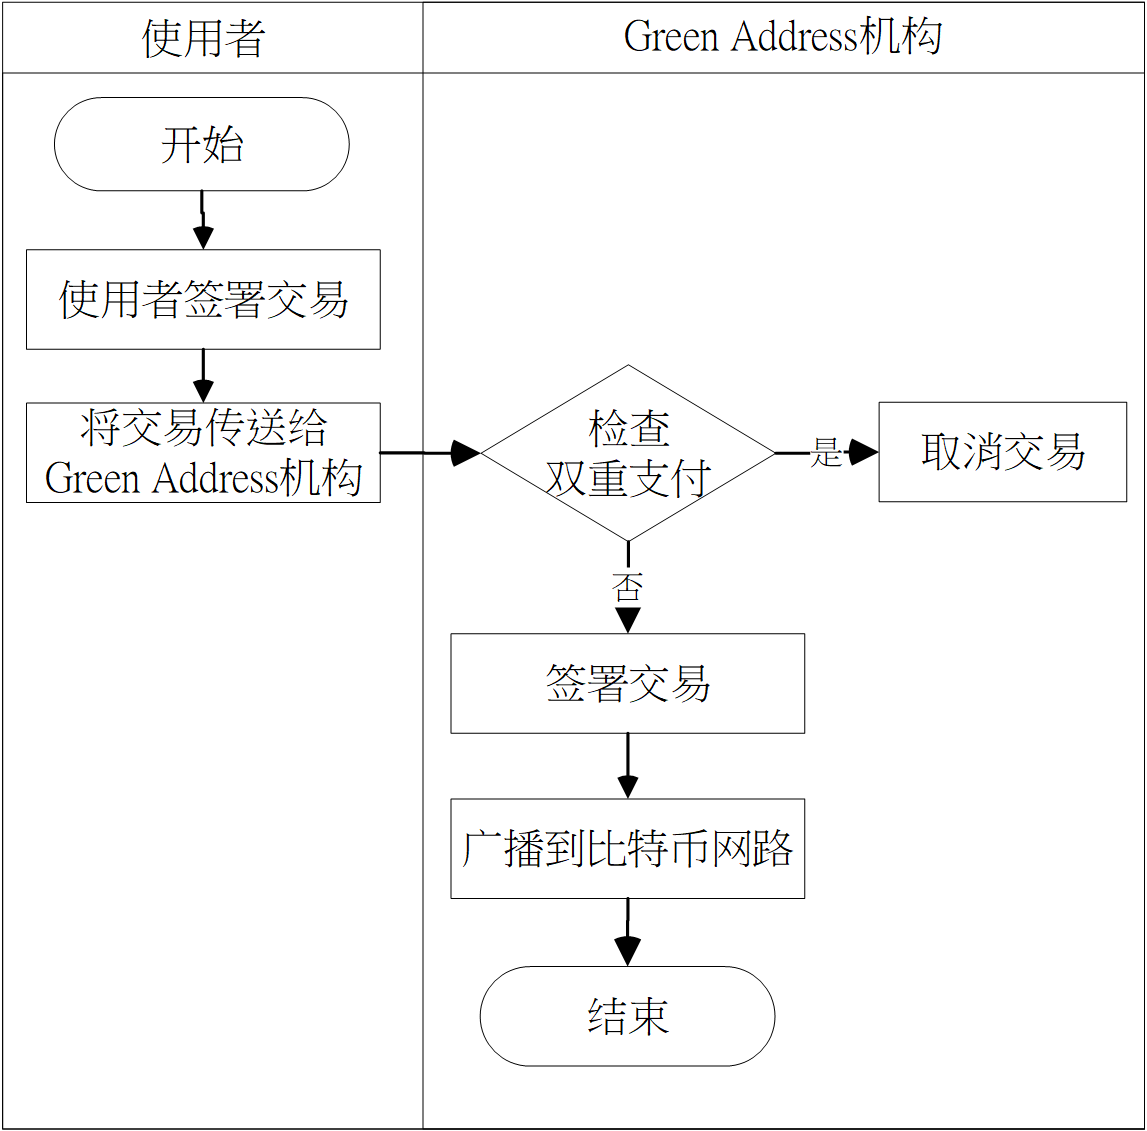
\includegraphics[width = .7\textwidth]{gatx.png}
				\caption{Green Address交易發起流程圖}\label{gatx}
			\end{figure}

			\begin{enumerate}
				\item 使用者使用原本創建Green Address的私鑰,並完成簽署交易。
				\item 因為是多重簽章地址,所以該交易需傳送至Green Address機構節點。
				\item Green Address機構節點收到交易信息後檢查該交易的發起地址是否存在雙重支付,倘若有雙重支付則遺棄;若無雙重支付則往下一個步驟。
				\item Green Address機構以Green Address的私鑰簽署該筆交易。
				\item 將該筆交易封包廣播至比特幣网络。
			\end{enumerate}

	\section{區塊鏈(Blockchain)}
	%區塊頭所有的結構
	自2009年以來,加密貨幣比特幣的誕生引發了新的貨幣革命浪潮,基於密碼學,點對點網絡,共識算法和區塊鏈技術,它們被結合成比特幣等加密貨幣。到目前為止,它在九年內發生大量的襲擊和欺詐事件後仍然在積極努力。 比特幣一直是互聯網上最具代表性的加密貨幣。比特幣是區塊鏈技術最重要的應用之一。我們將描述區塊鏈技術的一些細節。

		%%%%%%\subsection{本區塊大小的值 }
		\subsection{區塊頭(Block Header)}

		\begin{figure}[h]
			\centering
			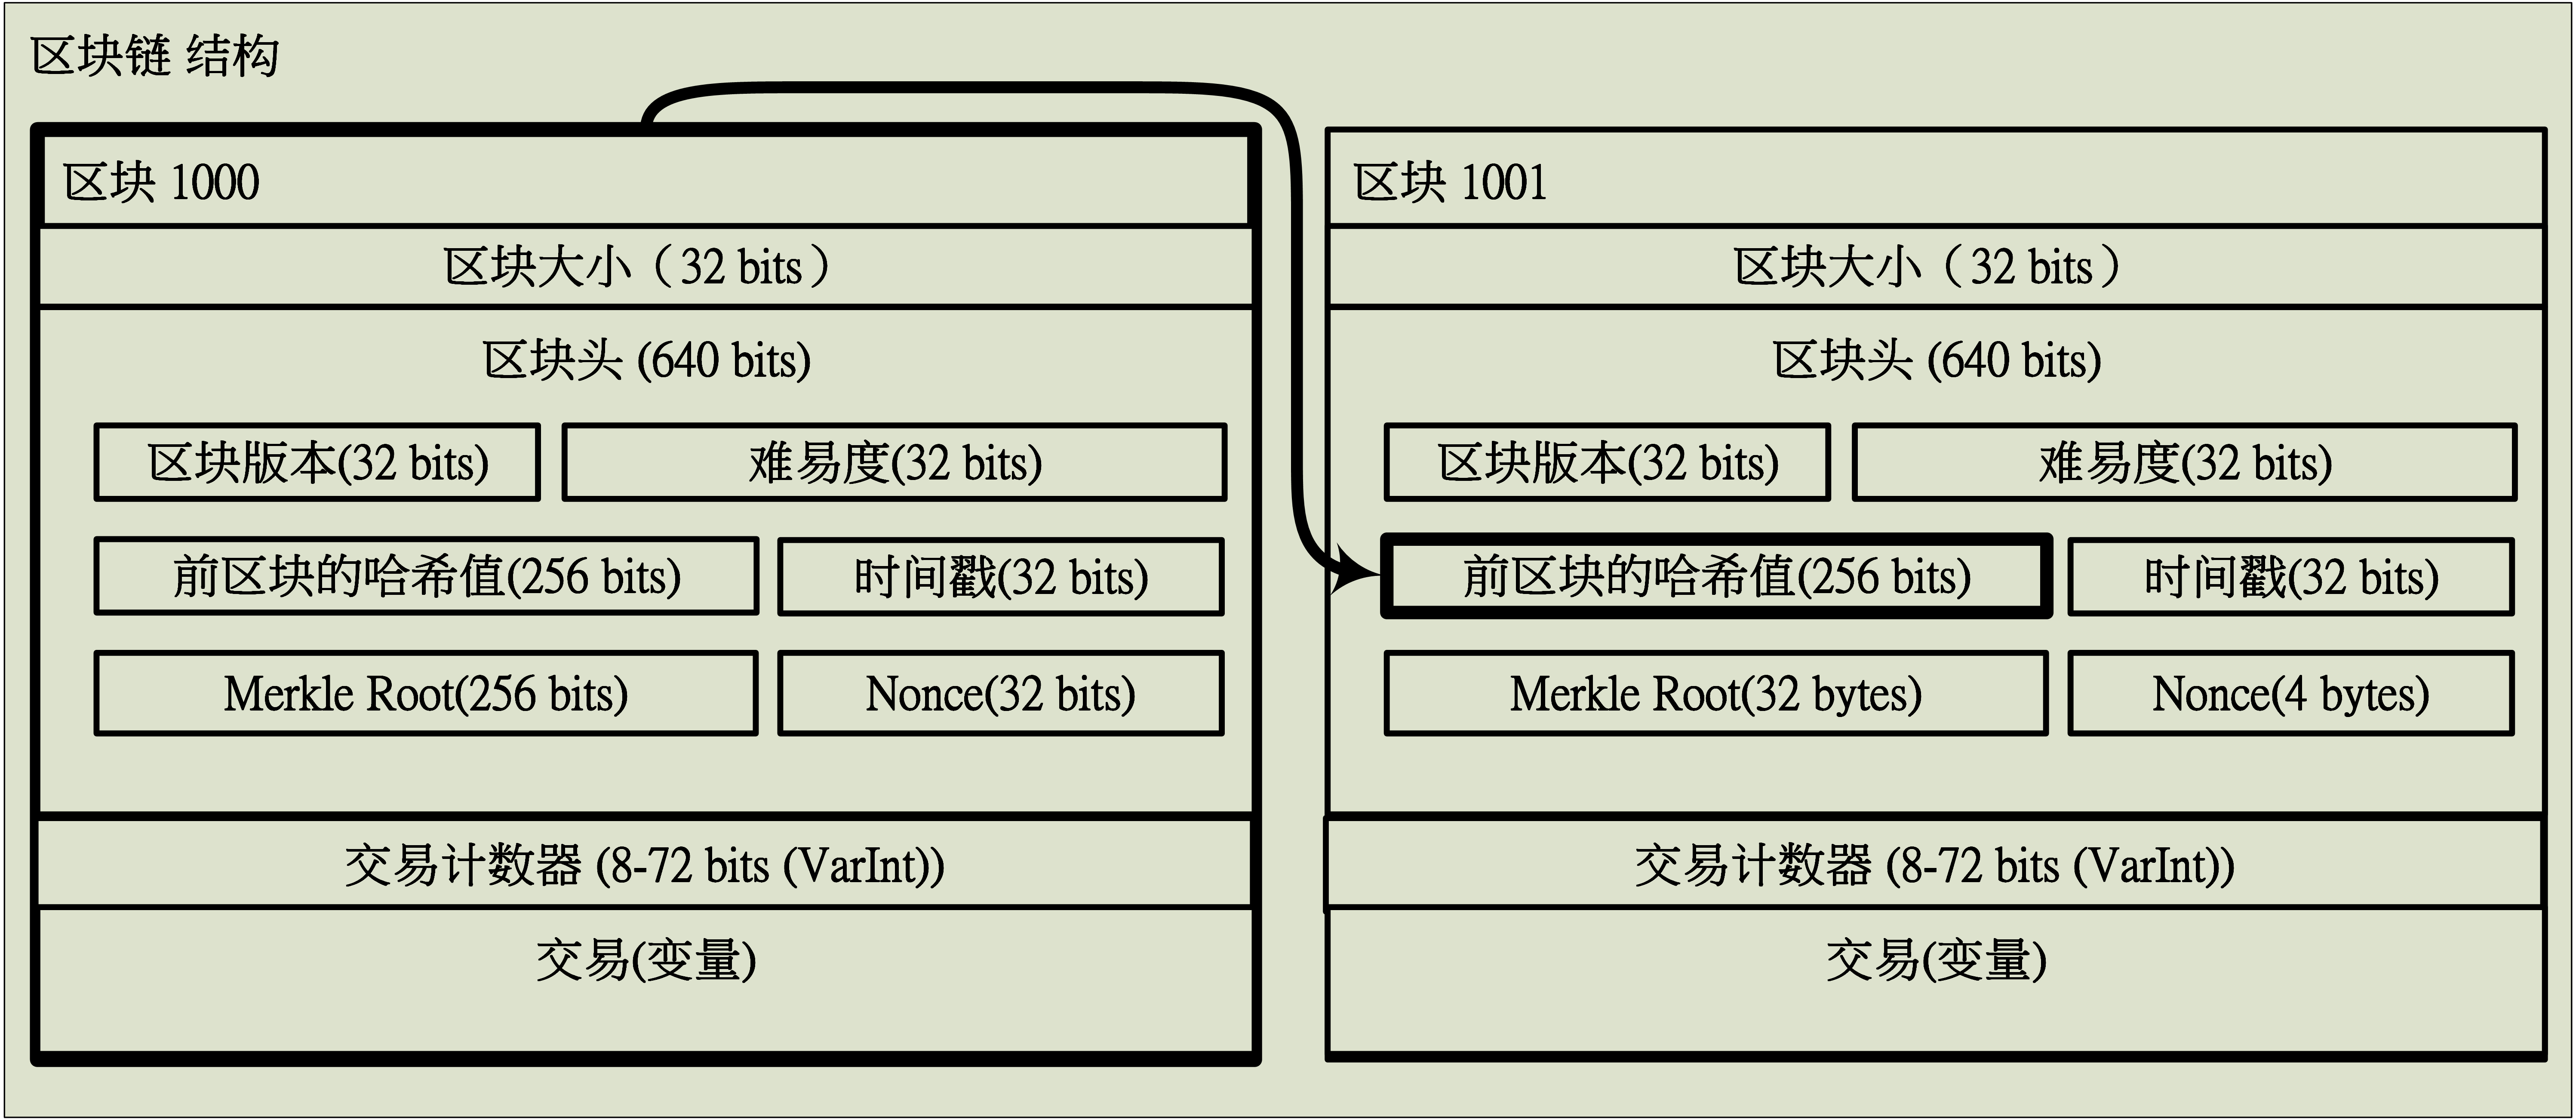
\includegraphics[width = 1\textwidth]{blockchain.png}
			\caption{比特幣區塊鏈結構圖}\label{blockchain}
		\end{figure}

			\paragraph{區塊版本(32 bits)}該欄位存儲比特幣區塊鏈中的區塊版本。
			\paragraph{前區塊的哈希值(256 bits)}記錄前一個塊的哈希值。 根據當前區塊的前一個區塊哈希值進而形成哈希指針,所有塊可以因為哈希指針連接在一起形成比特幣區塊鏈,不僅可以在區塊與區塊間建立虛擬鏈接,還可以使得區塊更難以被篡改。為新區塊不斷疊加在舊的區塊上,舊區塊的哈希值將繼續傳遞到最新的區塊。若區塊上面堆疊更多的區塊,促使的哈希值間接引用越多次,因此較早創建的區塊更難以修改。
			\paragraph{Merkle Root(256 bits)}Merkle Root的生成方法是將當前區塊的所有交易為n個進行排序後,此時的交易為n個樹葉,將每個樹葉進行一次SHA-256哈希算法取得哈希值得到$n$個哈希值,再將哈希值兩兩配對合併進行哈希,得到$n*2^{-1}$個哈希值後,在$k$輪後會使得$n*2^{-k}=1$時,合併到只剩下一個哈希值,最後一個哈希值則為Merkle Root,如圖所示\ref{MerkleRoot},在區塊鏈中的Merkle Root可用於快速檢查當前區塊中所有存儲交易的正確性。

			\begin{figure}[h]
				\centering
				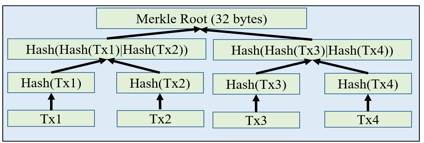
\includegraphics[width = 0.7\textwidth]{MerkleRoot.png}
				\caption{Merkle Tree示意圖}\label{MerkleRoot}
			\end{figure}

			\paragraph{難易度(32 bits)}在比特幣网络中難易度參數平均每十五天會有所變動,用以調控比特幣區塊的產出頻率,在過去的加密貨幣的設計中,有著因為沒有動態修改區塊難度,而導致區塊鏈生成速度太快,甚至導致區塊鏈系統崩潰。
			\paragraph{時間戳(32 bits)}以年、月、日、小時和秒的格式記錄區塊生成時間。
			\paragraph{Nonce(32 bits)}Nonce記錄著礦工在進行挖礦時,必須要不斷的嘗試Nonce參數,直到符合難易度參數,才可以創建一個全新的比特幣區塊。該值為32 bits ,意為著礦工嘗試的組態空間為$2^{32}$個可能性。

	%區塊內容 交易手續費攻擊
		%\subsection{Block Data}
		%	\subsubsection{交易計數器 (4-36 bits)}
		%	\subsubsection{交易信息}

	%\section{工作量證明(Proof of Work)}
	\section{點對點网络(Peer to peer network)}

	去中心化的加密貨幣系統帶給社會帶給傳統的中心化的金融體系以及政府帶來了很重大的衝擊,中本聰建構了一個不需要中央銀行發行貨幣的貨幣系統,在比特幣的貨幣發行上全靠區塊鏈既定的算法。除了貨幣發行,也將交易紀錄的帳本已明文的方式存儲在去中心化的區塊鏈中,以比特幣為例,現今的完整的比特幣區塊鏈帳本已經高達180GB,這樣保存完整交易數據的計算機稱之為全節點,在比特幣去中心化的网络中,如圖\ref{bitcoinfullnode}所示,截至2018年1月25比特幣网络中全節點數量為10552個\supercite{bitcoinfullnode},全節點的數量決定了比特幣帳本的可靠度,倘若有著更多的全節點,會使得比特幣网络堅不可摧,更難去修改歷史發生過的交易數據。

	\begin{figure}
		\centering
		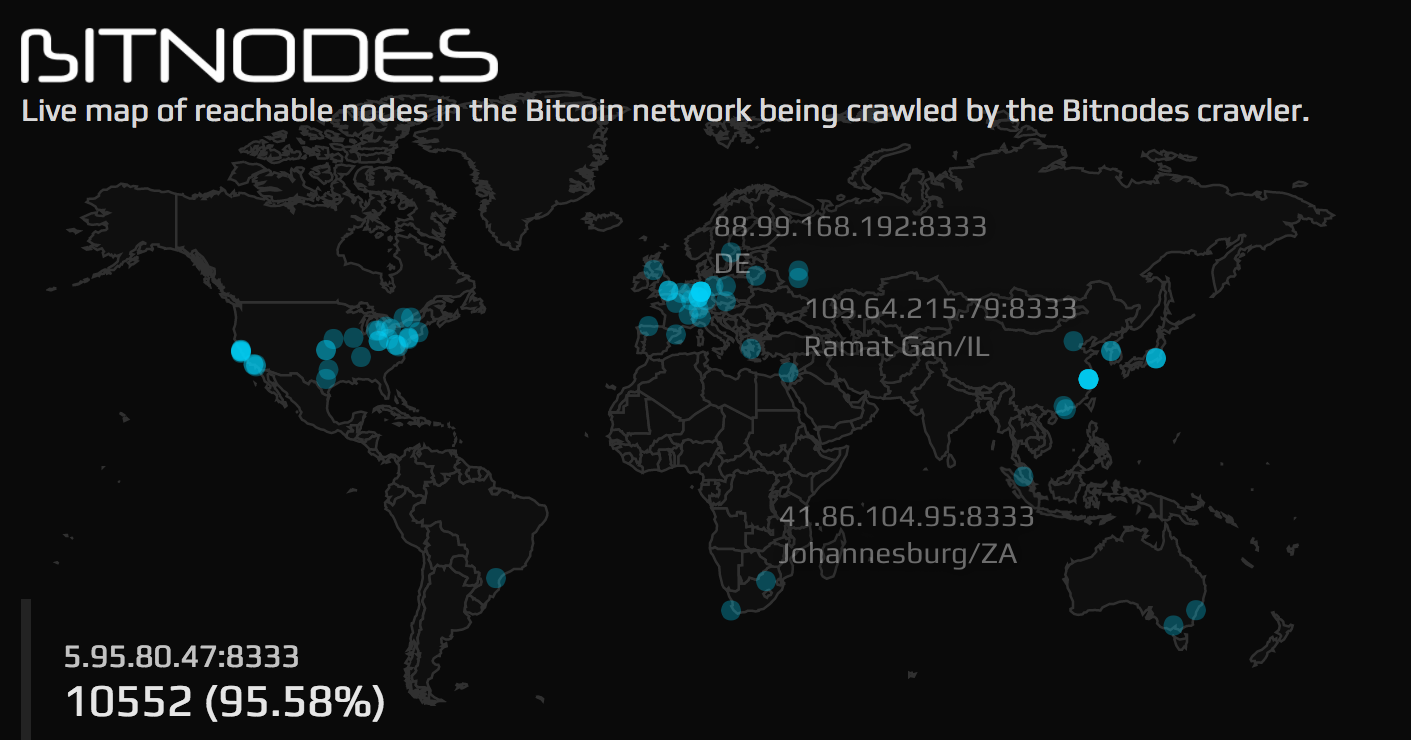
\includegraphics[width = .9\textwidth]{bitcoinfullnode.png}
		\caption{Bitcoin Full Node\supercite{bitcoinfullnode}}\label{bitcoinfullnode}
	\end{figure}

	% \section{山寨幣(Altcoin)簡介}

	% 	\subsection{萊特幣(Litecoin)}

	% 	\subsection{狗幣(Dogecoin)}

	% 	\subsection{域名幣(Namecoin)}

	% 	\subsection{以太坊(Etherum)}
	% Copyright (c)) 2014,2016 Casper Ti. Vecto
% Public domain 
\chapter{系统需求分析}

透过特性要因分析可以将比特币的交易监督系统大致分为四个主题,如图\ref{fish1}所示,分别为信息安全技术、加密货币钱包、近场通信技术以及数据库。作为⼀个⾦流系统,四项主轴之中信息安全是不可或缺的环节,着重于商家认证机制、用户权限控管、身份识别管理、用户访问控制四个方向;本系统致力于奠定匿名对实名的加密货币系统,必须对区块链技术、公钥私钥生成算法、点对点交易技术、钱包地址产出以及货币发行技术五个方向进行探讨;在交易场景中,本系统采用近场通信技术,因此需要对商品RFID标签建置、读取商品RFID标签以及Android Beam传输商品交易进行基础的API调研;为了使加密货币实名制的实现,数据库必须存储与政府和商家相关的信息。此时数据库加密、个人信息去识别化安全以及数据库连接便相当重要。
		\begin{figure}[!htbp]
			\centering
			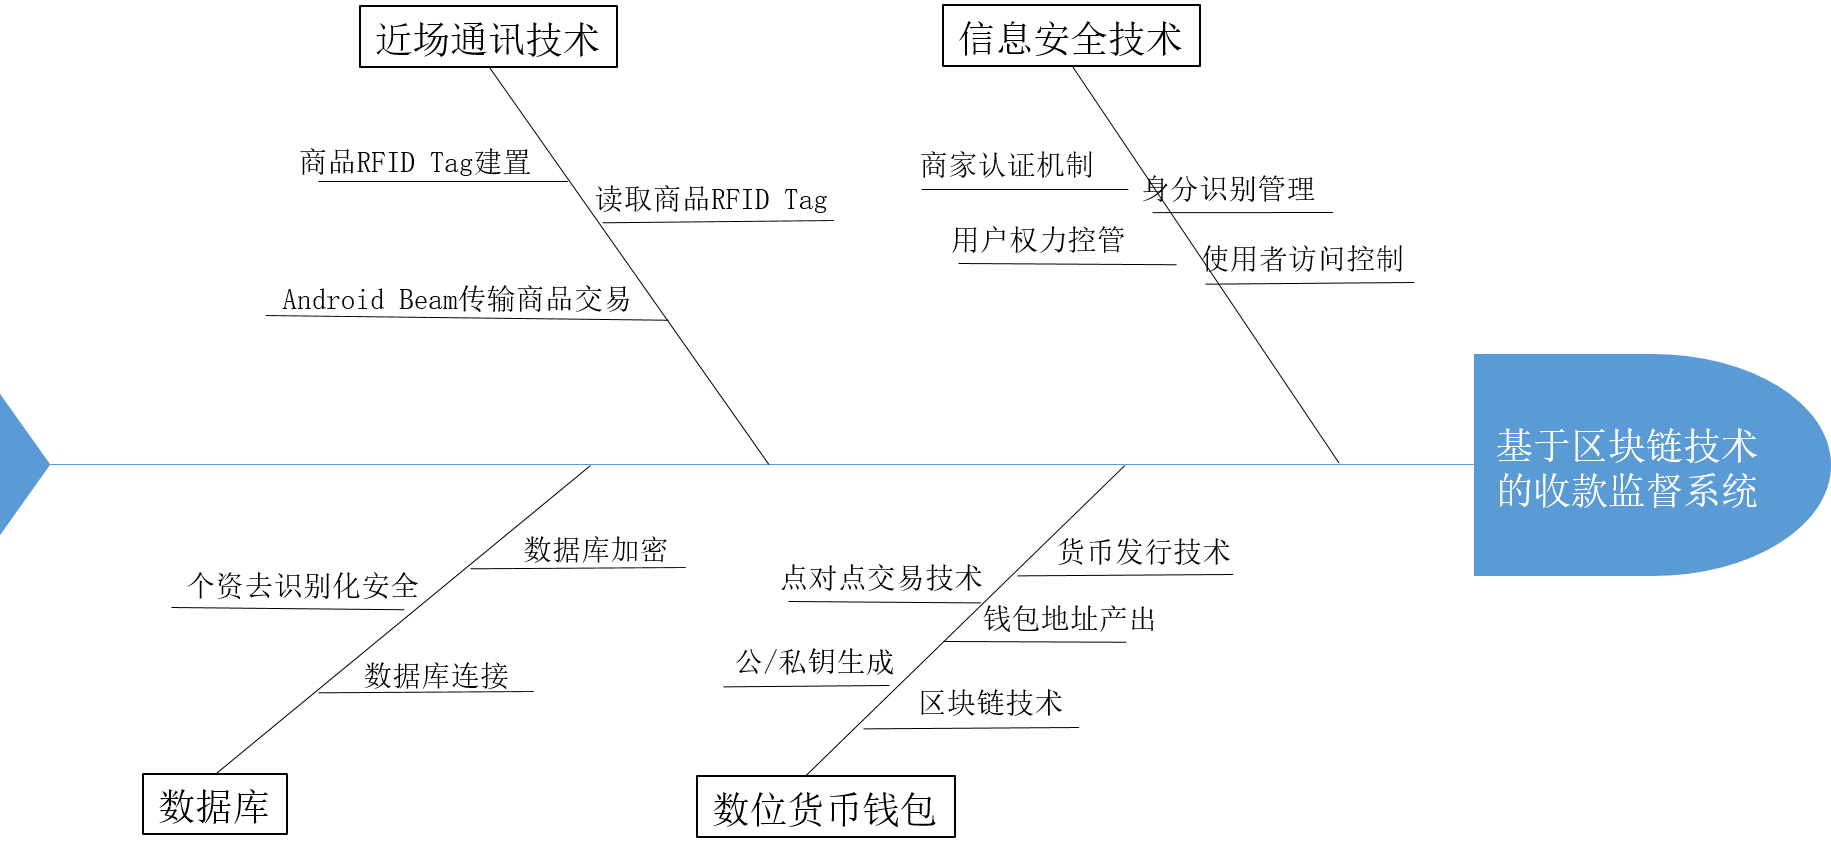
\includegraphics[width = 0.8\textwidth]{fish1.png}
			\caption{⽐特币的交易监督系统特性要因分析图}\label{fish1}
		\end{figure}

为了使本⽂所提出的系统设计之模块更加明确,对系统进⾏详细的需求分析可以使应确⽴的⽅向更加分明,在本章将分为三节进行分析,分别为交易模型分析、功能性需求分析以及非功能性需求分析。


\section{交易模型分析}

在设计比特币的监督系统之前必须针对现今社会中人与人之间的交易方式进行分析,在支付的方式依照使用人数比例大致可区分为现金交易以及电子支付两种类别,图\ref{modeall}为各种交易模型示意图。
%%fig allan
\begin{figure}[!htbp]
	\centering
	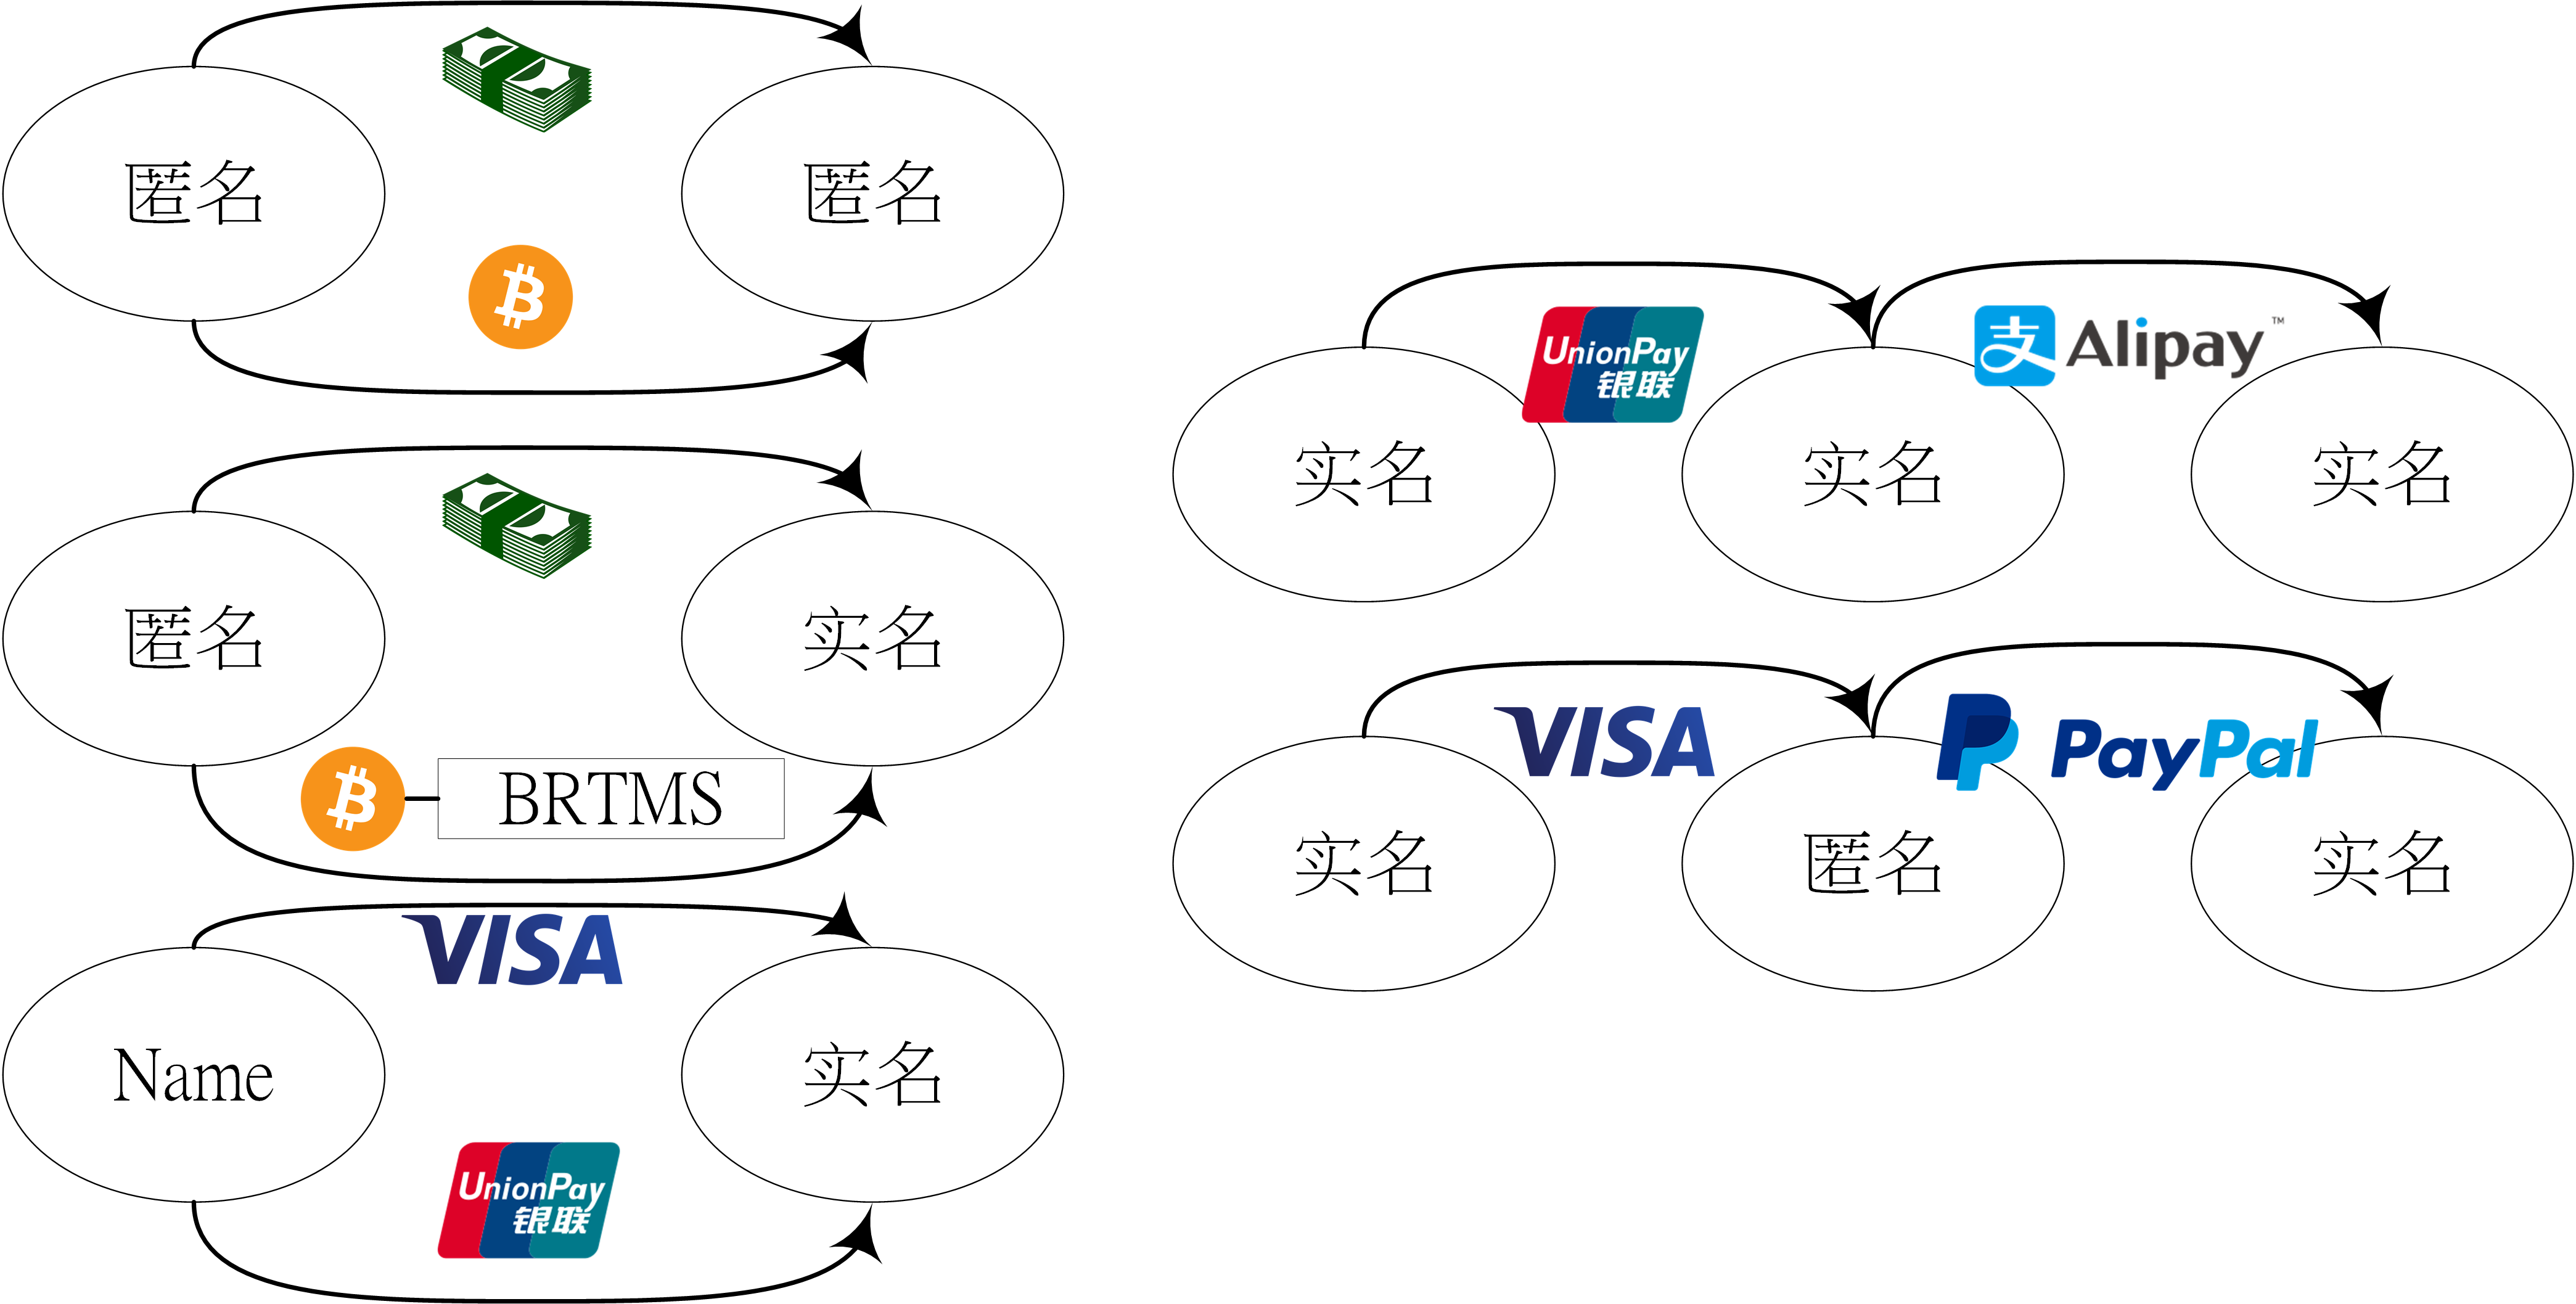
\includegraphics[width = 0.7\textwidth]{modeall.png}
	\caption{各种交易模型示意图}\label{modeall}
\end{figure}

	\subsection{现金交易类型}
	在现金交易模型中大致分为匿名顾客支付匿名商家以及匿名顾客支付实名商家两种,在过去的社会中,贝壳货币逐渐的被黄金取代,但黄金过于沈重在交易上相当不便。纸钞渐渐取代⿈⾦,法定货币的概念因此形成。法定货币包括钞票以及钱币,在过往的法定货币存在着黄金价值支撑,使得法定货币具有价值,但经过历史的变迁,已无⼤量的黄金作为法定货币的价值⽀撑,使法定货币渐渐地⾛向信⽤本位,纸钞以及铜币的使用皆不带有持有者的真实姓名,因此在现金交易模型分析中将顾客支付皆归类为匿名支付。

		\subsubsection{(一)匿名顾客支付匿名商家交易模型}
		现金法定货币的本身不存在用户信息以及交易信息。现⾦是一种匿名的支付方式,早期有许多的商家并无向政府进行注册,当顾客完成挑选商品进行结帐的同时,顾客只是将现金货币交付给商家,商家将商品卖给顾客,但在这过程中并无开立交易凭据。在商家无开立交易凭据的情况下,顾客完成此次的交易后,倘若该商品存在着瑕疵,进而引起商家与顾客之间的消费纠纷,使其在追溯的过程中存在没有凭据的困扰。对于匿名顾客支付匿名商家可以保有顾客的信息隐私,但无法保障顾客应有的顾客权益。政府因没有交易凭据而无法确认消费行为存在,使政府在课征税收的过程变得困难,且商家所贩售的商品并无得到明确的信息纪录,对于商家库存管理只能依靠过去的经验。对政府而言,商家贩售的商品并无完整的商品信息,无法对商家商品进行安全性检验,使得国民购买的商品存在的许多安全疑虑。

		\subsubsection{(二)匿名顾客支付实名商家交易模型}
		现⾦最为常⾒的匿名顾客⽀付给实名商家交易模式,在匿名顾客以现⾦法定货币进⾏交易时,商家只要开⽴交易凭据,即被归类为匿名顾客⽀付实名商家交易模型。商家在开⽴交易凭据的同时,凭据上所记载的信息包括职⼯信息、商家信息以及产品信息;职⼯信息记录该笔交易的担当人员,商家信息记录商家与顾客创建交易行为的时间与地点,产品信息详细记录顾客于该商家购买的商品;交易凭据因此成为记录交易事实的重要证明。对于顾客,因现⾦法定货币的匿名性使顾客依旧保有顾客信息隐私,但却因为商家开⽴交易凭据得以保障顾客权益。商家因为开⽴交易凭据使商家为实名,因为实名使得商家可以经营品牌形象。除此之外,因为凭据记录了产品信息让商家在库存管理以及收支计算变得更加容易。对政府⽽⾔,可以查看商家的所得以及商家贩售的商品,使政府可以更有效率的课征税收以及管理产品安全。

	\subsection{电子支付类型}
	电子商务的日趋盛⾏,电⼦支付交易模型也日渐普及,电子支付与加密货币的区块链技术不同的是采用数据库存储着所有的交易信息,而用户要能够使用电子支付也必须接受电子支付运营商实名制的条件。在电子支付的数据库中存在着黑客攻击、信息不一致以及中心化运营的风险,但电⼦⽀付有效解决了难以现金支付远距离之困境,也使得现今的网络购物变得更加发达。在电子支付交易模型中分为三种交易分别为实名顾客支付实名商家、实名顾客透过实名第三方再实名商家以及实名顾客透过匿名第三方再实名商家,以下将逐一说明。

		\subsubsection{(一)实名顾客支付实名商家交易模型}
		典型的实名顾客支付实名商家交易模式以VISA 国际电⼦⽀付公司为例,VISA 国际电⼦⽀付公司以下简称为VISA 公司,VISA 公司为中⼼化的运营,⽤⼾在使用VISA 电⼦⽀付以下简称为VISA 服务,前必须做详尽的用户真实⾝份认证,这使得VISA公司可以得到⽤⼾的所有信息,因此VISA公司拥有了允许或冻结相关⽤⼾⼾头的使用权限,并且为了保护用户隐私,所有的交易信息记录皆被存储在VISA 公司的数据库当中。

		VISA公司透过不断的优化电⼦⽀付技术已经可以接受每秒两千笔的交易量,为了维持稳定的运营服务,VISA 公司对每笔交易收取固定⽐例的⼿续费。在使用VISA 服务的过程中,顾客因为必须进⾏实名验证,使得顾客必须透露顾客个⼈信息,甚⾄可以针对这些个⼈信息进⾏商业上的交易。商家必须承担VISA 服务所需的交易⼿续费,成本因此提高,使得商品售价必须做出相对应的调整。对政府⽽⾔,因为交易信息皆以中⼼化的⽅式存储,可以⽅便的查看,也可以快速的查阅商家收⼊课征应缴的税收。
		

		\subsubsection{(二)实名顾客透过实名第三方支付实名商家交易模型}
		电⼦⽀付⽅式⽇趋普及也使用户可选择的电⼦⽀付渠道更加多元,较为常⾒的包括VISA 电⼦⽀付以及银联电⼦⽀付,⽽每⼀家银⾏为了让用户能在电⼦商务的⽀付上更为便利,会同时推广电⼦⽀付,使得银⾏卡⽀持电⼦⽀付,但更多的银⾏卡林⽴使得用户在卡⽚管理上更加繁琐,第三⽅的支付集成平台开始出现成为解决⽅案。顾客可以先在实名第三⽅⽀付后台添加多张卡⽚,再以第三⽅⽀付统一进⾏付款。实名顾客透过实名第三⽅⽀付给实名商家时,顾客可以得到更⽅便的银⾏卡管理,但却在第三⽅⽀付上透露了个⼈交易信息,面对仅⽀持第三⽅⽀付的商家却同时接受多家不同银⾏卡的⽀付⽅式,政府仅需要调阅第三⽅⽀付公司就可查阅该公司所有⽤⼾的交易信息,且可更完整的采集到商家的收⼊信息。
		
		\subsubsection{(三)实名顾客透过匿名第三方支付实名商家交易模型}
		为了让用户可以保有更多的隐私,Paypal 公司提出了实名顾客透过匿名第三⽅⽀付实名商家的模式,顾客欲⽀付⼀笔款项给商家时,⾸先使⽤VISA 服务⽀付⼀笔资⾦到Paypal 公司,Paypal 公司再以Paypal 的名义⽀付该笔款项给商家。换⾔之,商家不会取得相关的顾客个⼈信息,也无法对顾客交易信息进⾏数据挖掘。值得⼀提的是,原本透过VISA 公司⽀付款项给商家,顾客就必须先负担一笔的交易⼿续费给VISA 公司,而再透过Paypal 公司⽀付款项给商家时必须多经过Paypal 公司,顾客必须再⽀付第二笔交易⼿续费给Paypal 公司,这使得交易⼿续费更加的昂贵,但也因为多⼀个程序的资⾦转移,使得顾客的个⼈信息可以得到隐匿。实名顾客透过匿名第三⽅⽀付实名商家的交易模型,对顾客⽽⾔商家可以开⽴交易凭据使得顾客保有顾客权益,同时也保有顾客的匿名性,但缺点是顾客必须承担交易之间所增加的⼿续费;对于商家,可以透过交易信息管理商品库存,快速计算商家的收益;而政府则可以快速地查看商家交易信息以及商家所得。

		\subsection{交易比较}


		在上述两种现金交易模型与三种电子支付模型中可以看出,初始的交易型态为匿名顾客⽀付匿名商家交易模式,因无法保障顾客与商家之间的权益而发展出匿名顾客⽀付实名商家交易模式,这使得顾客与商家之间可以兼顾双⽅权益同时也保有顾客个⼈隐私,且可以让政府快速地查看税务相关信息。

		⽀付技术的⽇新⽉异与VISA 公司的出现,使得电⼦商务可以快速的运⾏,但也因为VISA服务会透露太多的个⼈信息,顾客需求逐渐转型成以实名顾客透过匿名第三⽅⽀付实名商家为基础的交易模式,兼具以电⼦⽀付作为付款⽅式,且同时保有个⼈隐私。但其缺点是需要多经过⼀个资金转移的程序,成为上述五种交易模型中交易手续费最为高昂的一种,但因其能保留顾客匿名性,让透过匿名第三⽅⽀付的模式在电子支付类型中依然成为顾客的第一选择。由上述分析可知,现⾦法定货币最佳的交易模型为匿名顾客⽀付实名商家交易模式,⽽电⼦⽀付类型的交易模式也趋向实名顾客透过匿名第三方支付给实名商家的方向演进。

		在使用加密货币作为交易货币的⽀付中,⼤部分的交易类型皆为如现⾦交易类型中匿名顾客⽀付匿名商家的交易模式,商家与顾客交易的过程中并无开⽴交易凭据,使得顾客与商家发⽣消费纠纷时因无法提出交易事实证明而无法拥有顾客权益保障。为了在使用加密货币时让用户可以同时兼顾顾客隐私与拥有顾客权益保障,也让商家不需要⽀付运营商比过去更为高昂的⼿续费并能以公开匿名的⽅式查看所有的交易信息,同时让政府在课征税收的业务上可以更加便利,本⽂致⼒于设计出三者都能同时兼顾的加密货币交易系统。表\ref{txvs}为交易关系⽐较表。


		\begin{table}[!htbp]
		\centering
		\caption{交易关系比较表}
		\label{txvs}
		\begin{tabular}{|l|l|l|l|l|}
		\hline
		 & 顾客 & 仲介单位 & 商家 & 商品 \\ \hline
		现金 & 匿名 & 无 & 匿名/实名 & 匿名/实名 \\ \hline
		VISA & 实名 & 无 & 实名 & 实名 \\ \hline
		支付宝 & 实名 & 实名 & 实名 & 实名 \\ \hline
		PayPal & 实名 & 匿名 & 实名 & 实名 \\ \hline
		加密货币 & 匿名 & 无 & 匿名/实名 & 匿名/实名 \\ \hline
		\end{tabular}
		\end{table}

\section{功能性需求分析}

在现今的加密货币交易系统中采用匿名对匿名⽀付的交易模式,这样的交易模式顾客无法拥有权益保障,商家需支付高昂的交易手续费,政府也无法在交易中课征税收。传统交易模式中所采用实名⽀付给实名的交易模式虽然可以有效地保障顾客权益,但在这对顾客个⼈隐私⽇趋重视的世代中,个⼈信息越来越有价值,个⼈信息的保护更是成为重要的课题。在本系统中,将以加密货币-⽐特币为基础,设计⼀个以匿名顾客⽀付给实名商家为基础的比特币交易监督系统。在实现匿名⽀付给实名的交易模型同时,也将商家的库存信息同时加⼊,使商家也可以轻松地使用本系统管理产品库存。如图\ref{UC}所示,在本系统中,参与者总共有三种,分别为商家、职⼯以及顾客。

商家,在本系统中为第⼀个参与者,因为必须要有商家的注册参与,才可以进⼀步的添加职⼯以及商家产品信息,如此⼀来商家才有商品可以贩售。参与者商家本⾝有三项需求,分别为⽤⼾注册与登⼊、职⼯管理以及商家产品管理。以下将逐⼀说明:


	\begin{enumerate}
	\item 用户注册与登入:为了得到政府的认证,商家必须接受政府的查看,提交相关的信息到本系统中。在用户注册的页面当中,进行用户的注册或是登入都需要用户信息,因此需要包括加载用户信息。
	\item 职工管理:在完成用户注册与登入之后,才得以进行职工管理,商家本身会有大于或等于一个职工的帐号,商家的注册者本身会是一个职工。在职工管理当中,需要有查找职⼯帐⼾与修改职⼯帐⼾两项功能,查找职工帐户的功能必须包括加载职工信息。在进行职工帐户修改时需要包括职工信息以及商家信息,才得以对职工信息进行修改。
	\item 商家产品管理:商家需要添加产品信息至商家产品信息中,产品为政府认可的产品认证编号,在本系统中产品本身不存在价格,需要参与者商家将产品添加至商家产品信息中才可以添加价格,这样的设计可以让不同的商家在不同的产品设置不同的价格。除了商家对商家产品价格需求,同时也需要对产品库存进行管理,透过区块链加密货币公开交易信息的特性,可以使得库存管理以及交易信息更快速地核对。在商家产品管理中需要查找产品信息,在查找产品信息的同时包括加载产品信息,使得查找过程可以顺利运作。在查找完成产品信息后,商家需要将产品信息与商家信息添加到商家产品信息当中,在这过程中需要包括加载商家信息以及商家产品信息。

	\end{enumerate}

职⼯,需要进⾏⽤⼾注册并且通过政府的审查,在完成审查之后需要进⼊商家交易管理建置移动收银机。参与者职⼯本⾝有两项需求,分别为⽤⼾注册与登⼊、及商家产品管理。以下将逐⼀说明:


	\begin{enumerate}
	\item 用户注册与登入:要成为职工之前职工需要进行用户注册,等待政府的审查之后,并经由商家进行职工管理将用户与商家一并提交到职工信息,才得以成为正式的职工,职工的用户注册与登入皆需要包括加载用户信息,才能使得注册与登入功能顺利运行。
	\item 商家交易管理:在完成登入后,商家交易管理将会加载相关信息,包括加载职工信息,在交易信息中添加职工编号,加载商家信息使得在进行交易的过程中可以将商家的比特币地址发送给顾客等待接收款项以及加载商家产品信息使得职工的移动设备上可以显示所有的商家产品信息,在完成信息加载后职工的移动设备已经成为一台移动收银机。在职工在进行扫码的过程会创建交易清单并且将交易清单发送给顾客等待顾客的付款。在等待付款时,商家交易管理需要认证该笔交易是否有效,因此需要加载交易信息,
	\end{enumerate}

顾客,为了保持顾客的身份匿名,参与者顾客与参与者职工和商家不同,顾客在参与本系统的同时不需要注册帐户以及登入用户帐户,顾客主要需求为加载过去与顾客相关的交易信息,以及使用比特币支付进行付款:


顾客交易管理:顾客需要加载交易信息,但因为交易信息中的信息并无详细阐述商家产品信息,因此需要进一步加载商家产品信息使得交易明细更加的清楚。除了显示过去的交易信息的需求,顾客更需要创建一笔交易以⽐特币进⾏付款。待付款完成之后,等待参与者商家向顾客回复⽀付完成即确立该笔交易完成。

	\begin{figure}[!htbp]
	\centering
	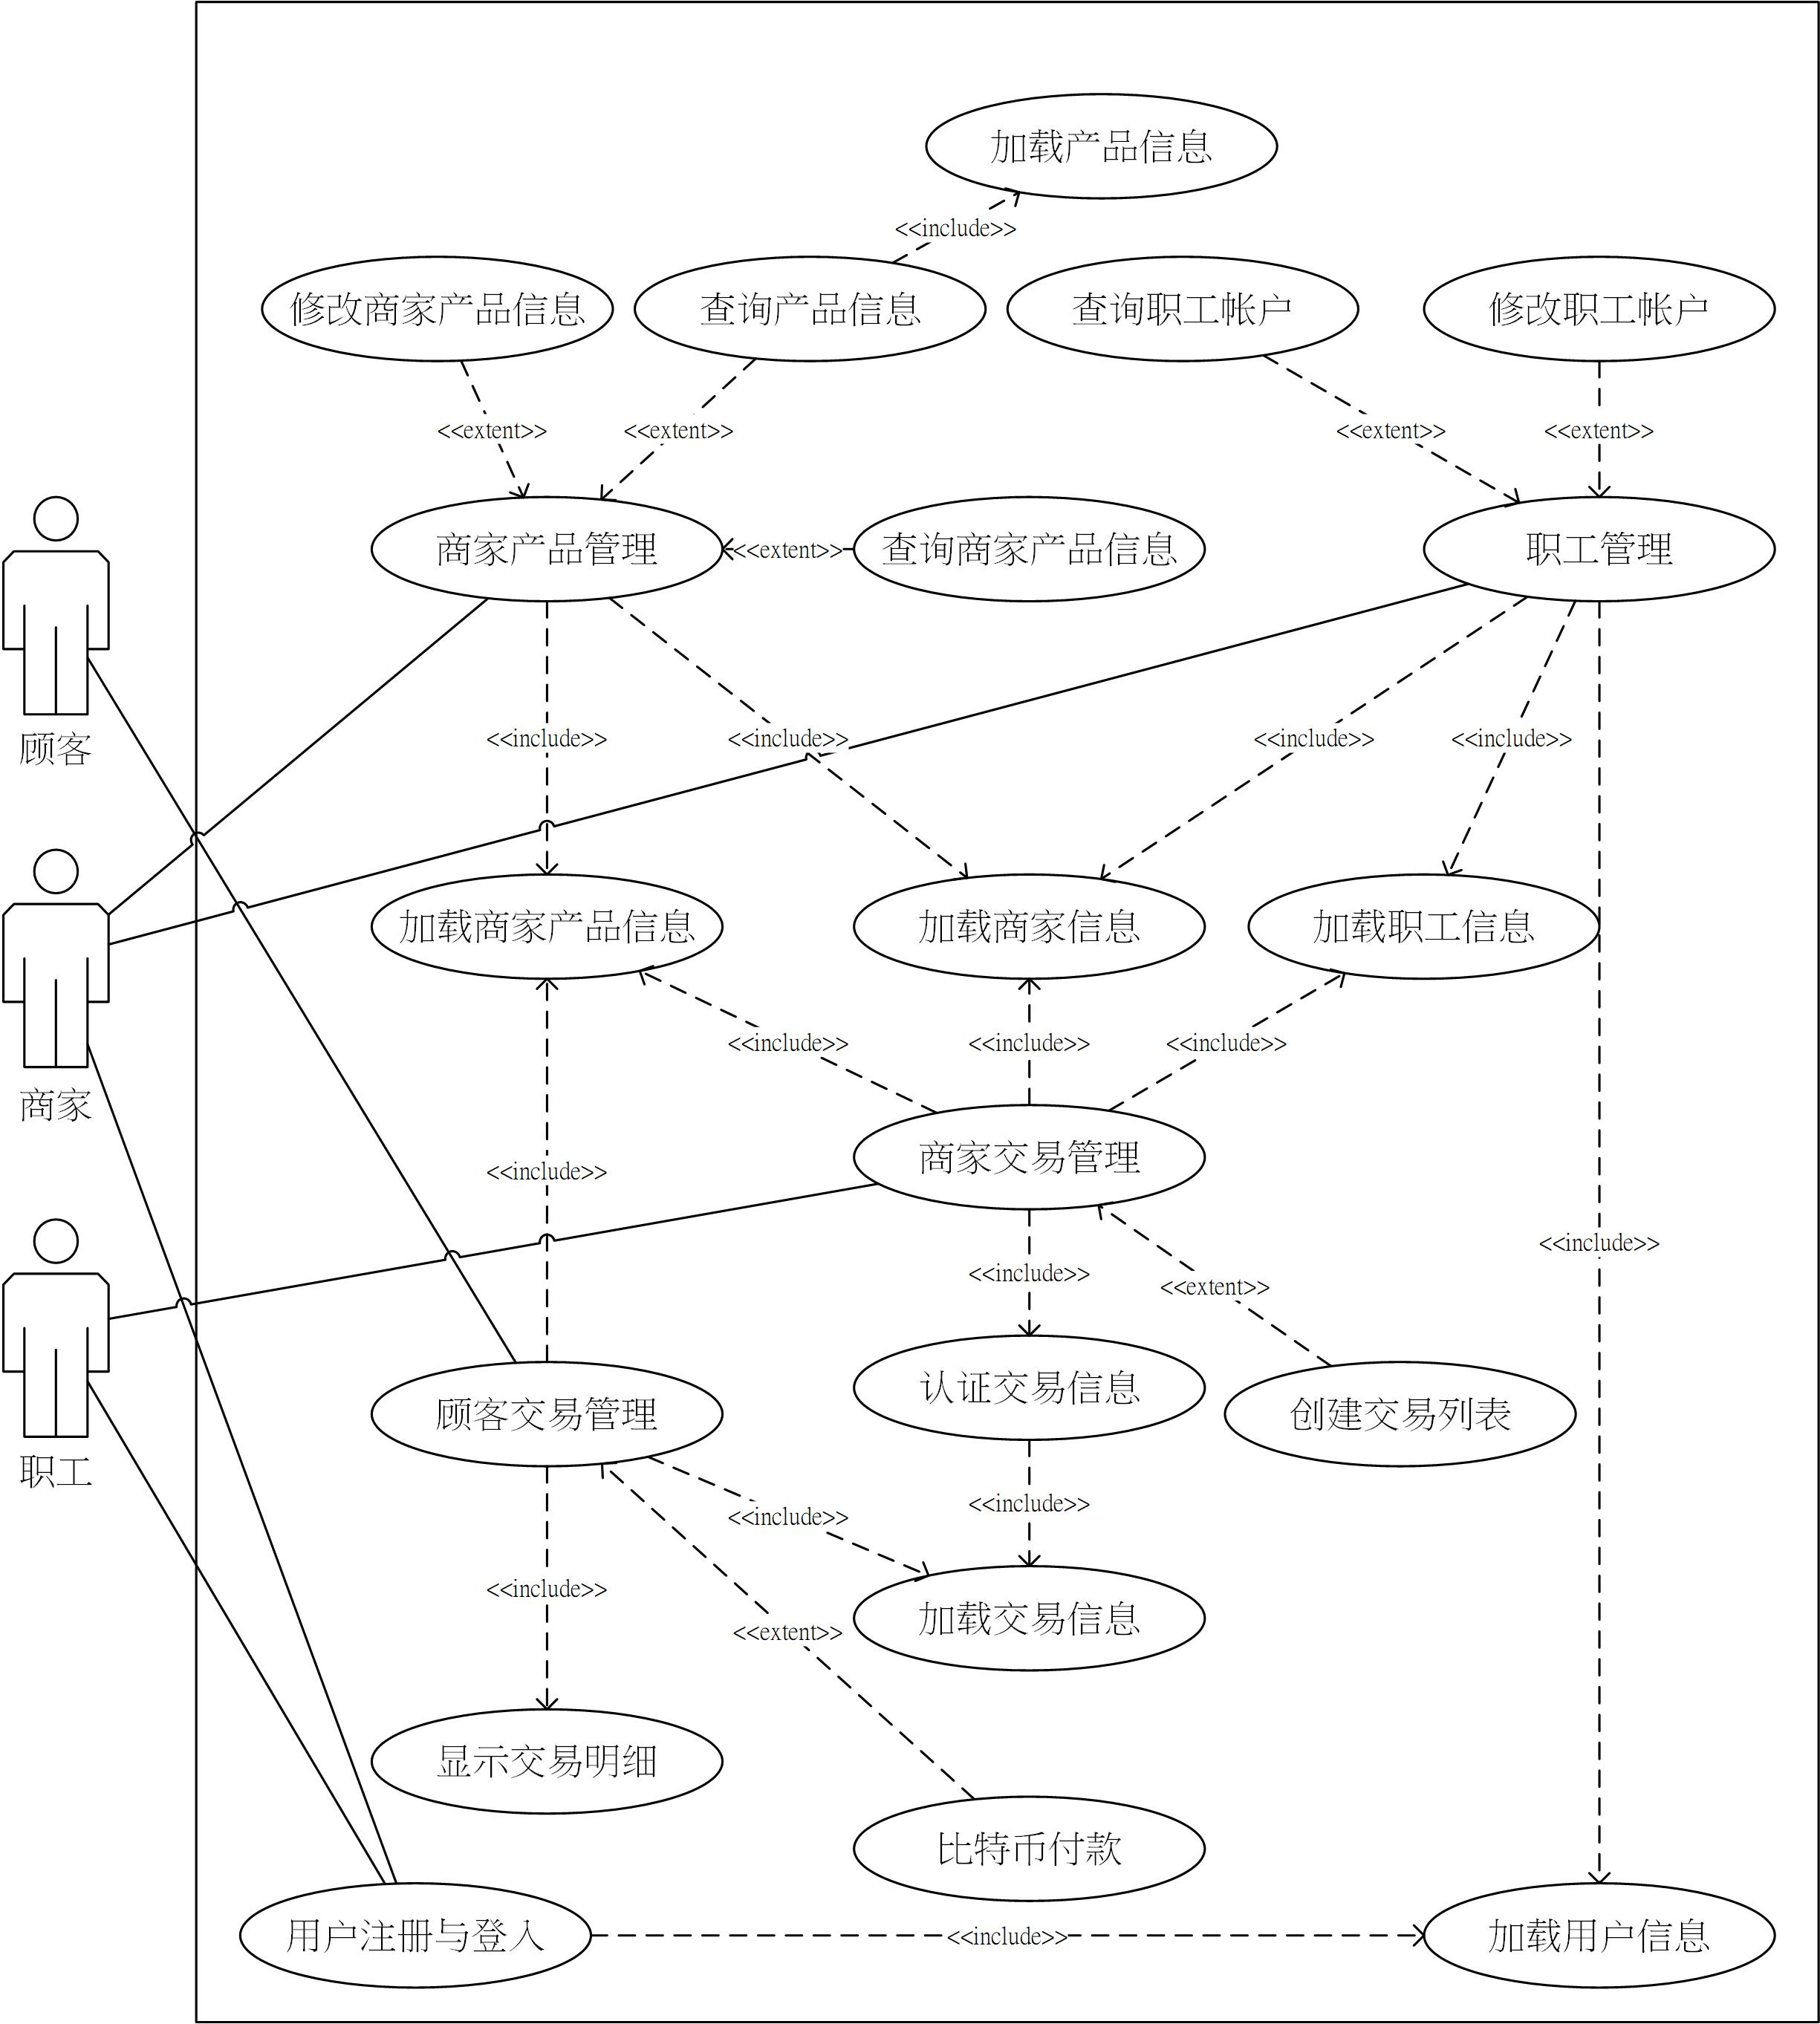
\includegraphics[width = 0.9\textwidth]{UC.jpg}
	\caption{比特币交易监督系统⽤例图}\label{UC}
	\end{figure}

	\section{非功能性需求分析}

	\subsubsection{(一)性能需求}
	
	本文所实践之系统为比特币的交易监督系统,参与者商家需要使用到商家端建置与管理商品信息子系统,在参与者商家操作该子系统时,系统在设置完成后,于存储的过程中应于三秒内完成。于商家端建置与管理商品信息子系统、商家端行动收银与交易明细系统应达到于两秒内完成子系统与数据库之间的信息传递以及信息存储,倘若商家与顾客在完成交易后,却无法得到快速的系统响应,这使得参与者顾客与职工收到⽀付完成的回复,甚至导致商家的交易塞车影响用户的消费体验。

	\subsubsection{(二)可拓展性}

	本论文提出的系统为比特币的交易监督系统雏形,于系统设计中将优先考虑最必要功能并加以实现,包括商家端建置与管理商品信息子系统、商家端行动收银与交易明细系统以及客户端行动支付与交易明细系统,于上述三个子系统中皆可以进行数据库字段的添加,使得交易信息、商家信息、商品信息、商家产品信息、用户信息以及职工信息更加的完备且更符合实际上业务需求。在未来甚⾄可以加⼊更完整的税务信息,使政府在税务计算⽅⾯可以大幅降低⼈⼒资源成本且更快速地进⾏税务统计,而库存管理⽅⾯可以加⼊库存预测的服务。

	\subsubsection{(三)可操作性}
	在本系统中的三个⼦系统中,为了将商家端⾏动收银与交易明细系统,以及客户端⾏动⽀付与交易明细系统实现在⼿持移动设备Android 操作系统上,于介⾯设计⽅⾯应给予商家⽤⼾以及顾客⽤⼾⼈性化的操作交互设计,以及于代码撰写⽅⾯应更加简洁,使得⽤⼾在启动本⼿持移动端应⽤程序时可以在最短的时间内完成初始化程序加载。除了针对⽤⼾交互⽅⾯的优化,也需要添加各个功能项⽬的使⽤说明,以及⽤⼾操作问题反馈,给予使用本系统的移动设备在应⽤程序上能快速的修正以提升⽤⼾体验。商家端建置与管理商品信息⼦系统是以Java 编程语⾔实现,针对参与者商家操作进⾏设计,该⼦系统需简单明确的呈现商家信息、产品信息以及商家产品信息,使参与者商家可以快速地查看所有商品,并添加、修改以及删除相关产品信息,包括价格、库存以商家产品描述。

	\subsubsection{(四)软件与硬件环境需求}
	表\ref{eva}为本文提出系统的软件与硬件环境需求,商家交易客户端与顾客交易客户端是建置在Android手机的应用程序,本文提出的交易方式为比特币,因此导入bitcoinj\supercite{Bitcoinclients}对比特币钱包进行管理,该套件可以生成比特币地址、同步比特币区块链、透过AES加密算法保护比特币钱包以及发起比特币交易至比特币网络。针对数据库的控制数据传输选用JDBC\supercite{JDBCdatabaseaccesswithJava:atutorialandannotatedreference}实现数据库的添加、修改、删除以及查找的功能,商家交易客户端与顾客交易客户端的手机移动设备必须要内置NFC传感器用来发送与接收交易信息。商家管理客⼾端是以Java 编程语⾔实现,软件环境中需⽀持Java ⼯作环境,服务器端则需要SQL 环境进行数据库搭建。


	\begin{table}[!htbp]
	\centering
	\caption{环境需求表}
	\label{eva}
	\begin{tabular}{|c|c|c|c|}
	\hline
	- & 操作系统 & 软件 & 硬件 \\ \hline
	\begin{tabular}[c]{@{}c@{}}商家交易\\ 客户端\\ 与\\ 顾客交易\\ 客户端\end{tabular} & \begin{tabular}[c]{@{}c@{}}Android 4 \\ 或以上\end{tabular} & \begin{tabular}[c]{@{}c@{}}Java 7 或以上 \\ bitcoinj v0.14.6 \\ JDBC 4.2 或以上\\  Maven 3+\end{tabular} & \begin{tabular}[c]{@{}c@{}}存储容量:32GB\\ 内存容量:2GB\\ 网络需求:10兆或以上\\ 传感器:NFC传感器\end{tabular} \\ \hline
	\begin{tabular}[c]{@{}c@{}}商家管理\\ 客户端\end{tabular} & \begin{tabular}[c]{@{}c@{}}Windows 7 \\ 或以上\end{tabular} & \begin{tabular}[c]{@{}c@{}}Java 7 或以上 \\ JDBC\end{tabular} & \begin{tabular}[c]{@{}c@{}}硬盘容量:100GB\\ 内存容量:4GB\\ 处理器:Core 2 Duo 或以上\\ 网络需求:10兆或以上\end{tabular} \\ \hline
	服务器端 & \begin{tabular}[c]{@{}c@{}}Windows Server \\ 2003 \\ 或以上\end{tabular} & \begin{tabular}[c]{@{}c@{}}Microsoft SQL Server \\ bitcoin-qt 0.8.X 或以上 \\ Apache HTTP Server\end{tabular} & \begin{tabular}[c]{@{}c@{}}硬盘容量:1000GB\\ 内存容量:16GB\\ 处理器:Xeon E3 或以上\\ 网络需求:100兆或以上\end{tabular} \\ \hline
	\end{tabular}
	\end{table}




%		\begin{figure}[!htbp]
%			\centering
%			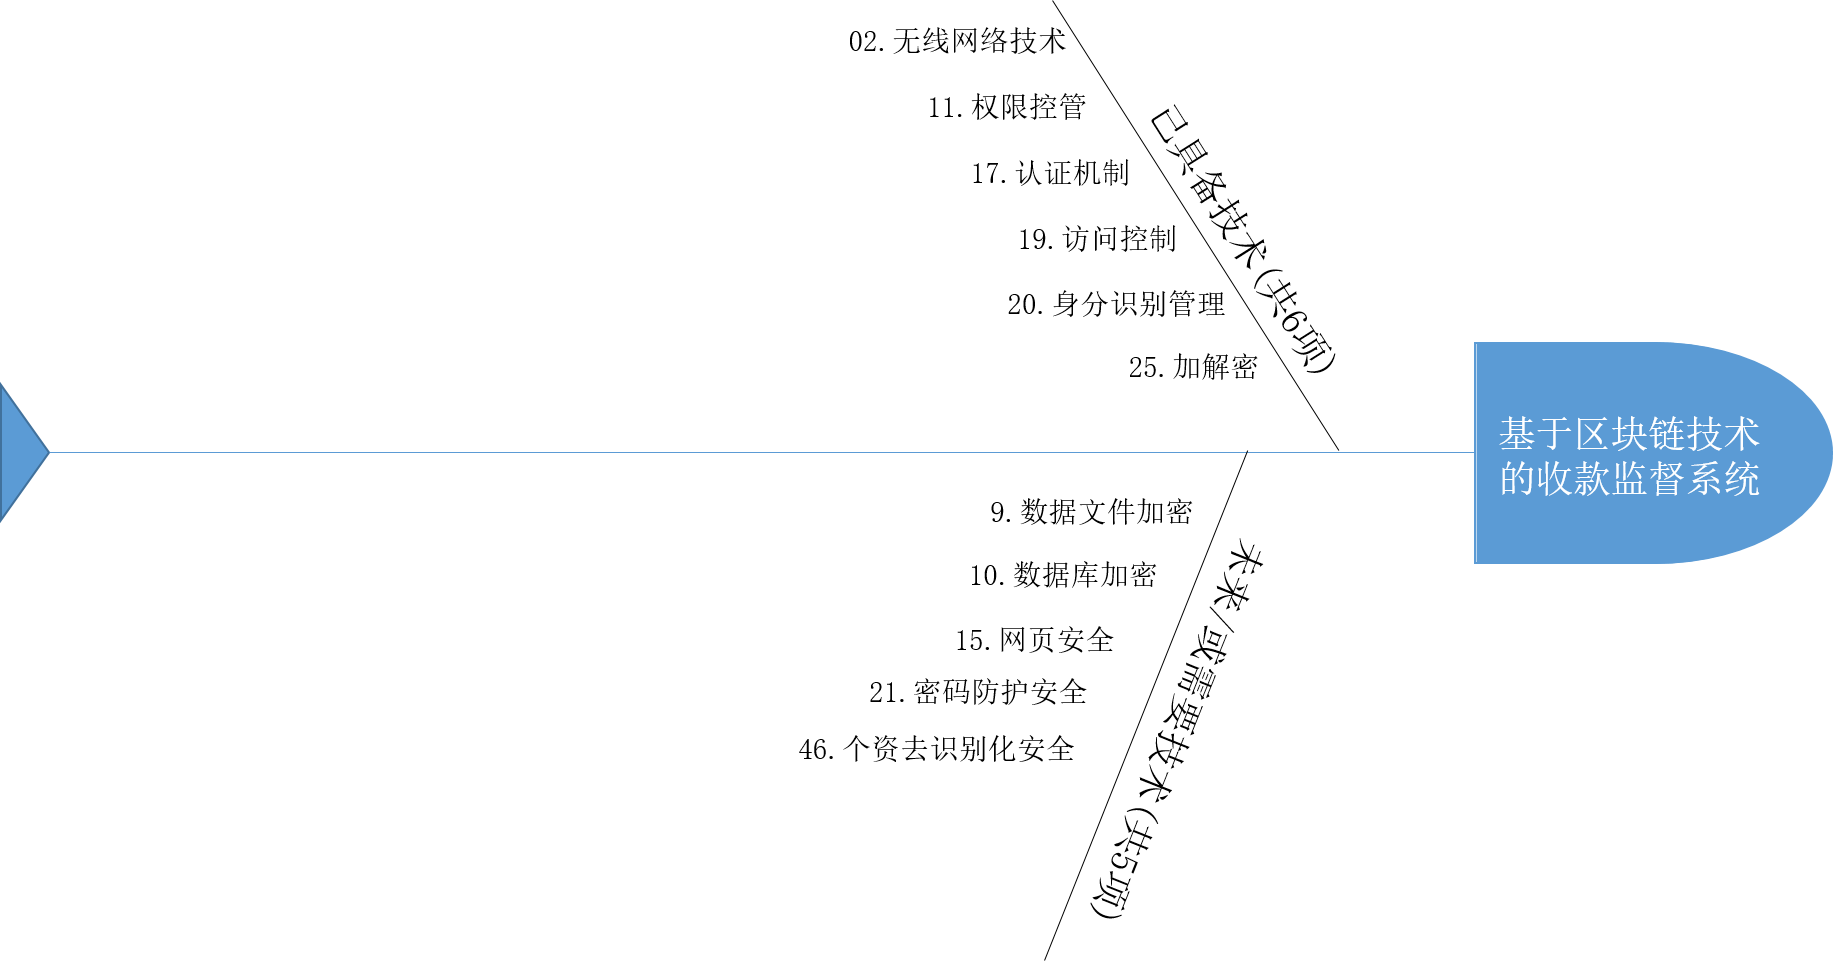
\includegraphics[width = 1\textwidth]{fish2.png}
%			\caption{鱼骨图(2)}\label{fish1}
%		\end{figure}

%		\subsection{匿名顾客对匿名商家}
%	\section{各种交易模型比较}

	% Copyright (c) 2014,2016 Casper Ti. Vector
% Public domain.

\chapter{区块链的实名交易监督系统設計}
%\pkuthssffaq % 中文测试文字。
本論文提出区块链的实名交易监督系统(Blockchain Real-name Transaction Monitoring System,BRTMS),以下簡稱BRTMS,BRTMS以密碼貨幣比特幣實作,BRTMS包含三個子系統,商店和商品信息管理子系統(Store and Merchandise Information Management Sub-System,SMIMSS)、商家移動裝置收款及交易子系統(Store Mobile payment Collection and Transaction、Sub-System,SMCTSS)、客戶端移動支付和交易子系統(Client Mobile Payment and Transaction Sub-System,CMPTSS),我們將在稍後描述這些子系統。

	\section{BRTMS數據庫設計}

		\subsection{原數據庫}
		区块链的实名交易监督系统應用了四個原數據庫,分別為使用者數據庫、產品數據庫、商家數據庫、交易數據庫:

		\begin{figure}[h]
			\centering
			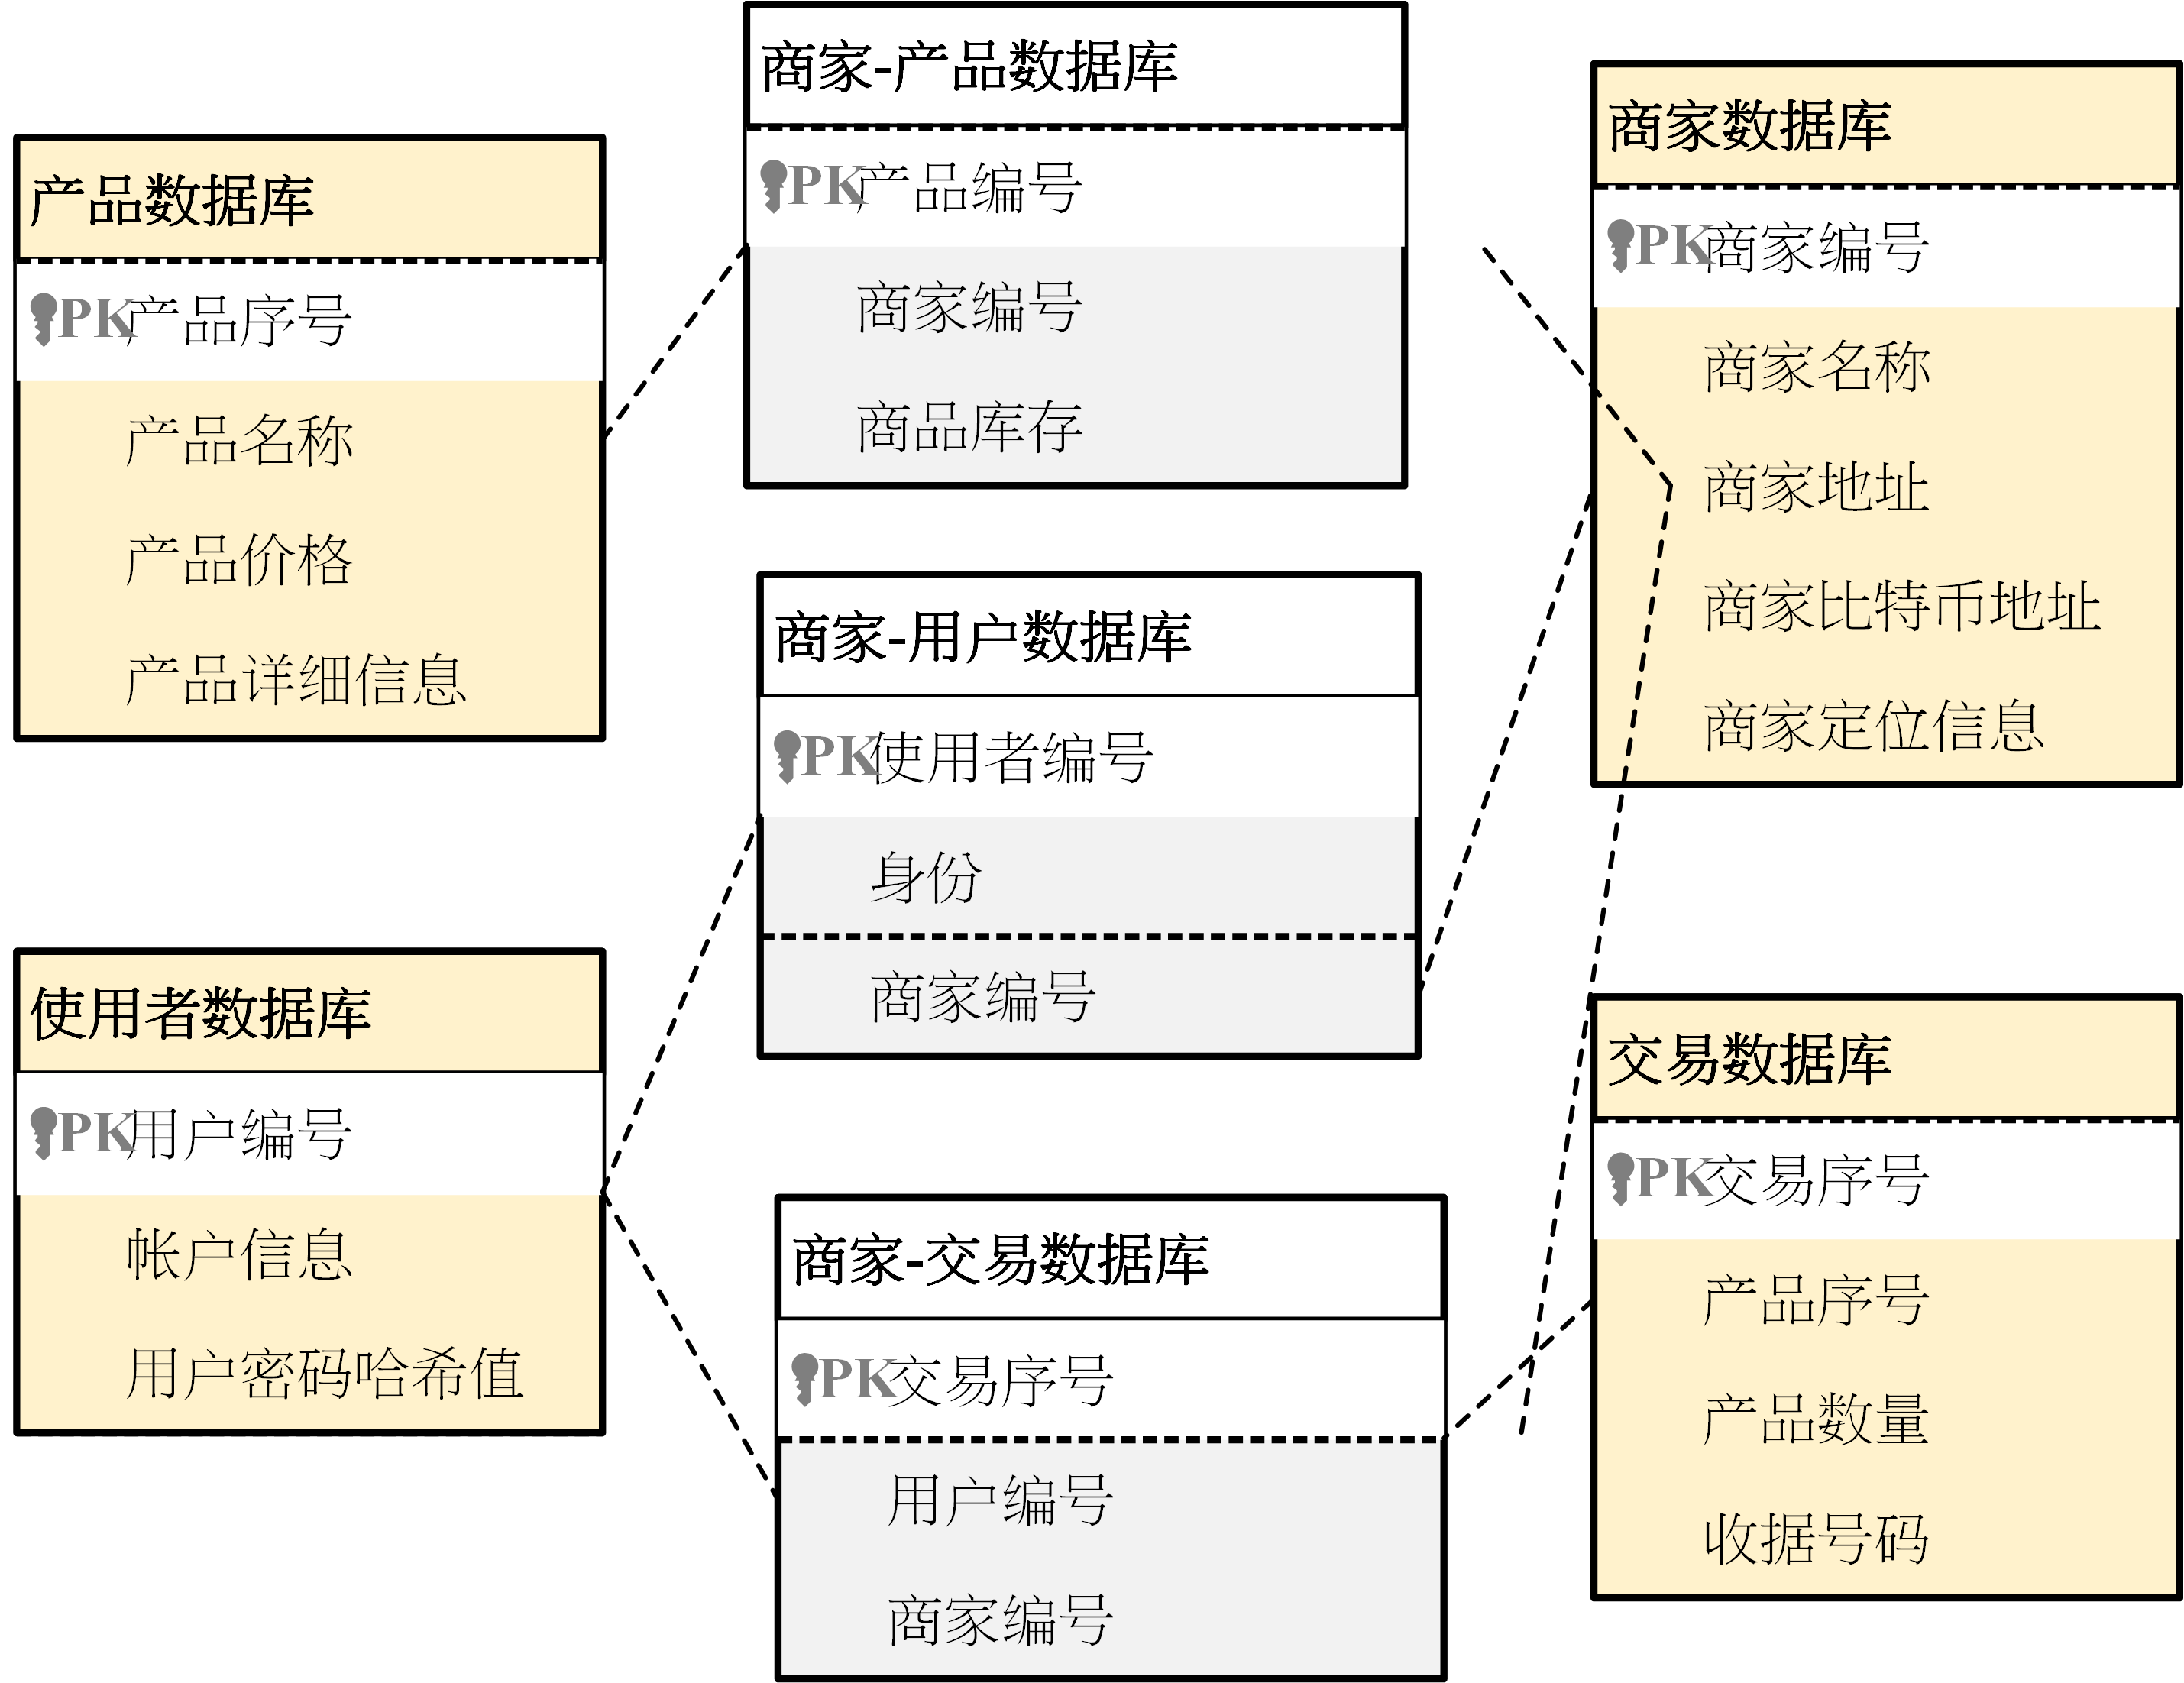
\includegraphics[width = 0.8\textwidth]{db.png}
			\caption{BRTMS 數據庫}\label{db}
		\end{figure}

			\paragraph{店家數據庫}存儲正在審核中的企業信息或已經過審核的企業信息。存儲的信息包括商家ID、商戶名稱、商戶位置、商戶的密碼貨幣地址以及GPS坐標。
			\paragraph{產品數據庫}只有授權用戶才能登錄添加或修改交易產品信息。產品數據庫內容包括產品標識號、產品名稱、產品說明、日期和價格等相關信息。
			\paragraph{交易數據庫}記錄包括交易序列號、產品識別號碼、產品交易金額、商戶密碼貨幣收款人地址、消費者密碼貨幣支付地址、商戶ID和最後確認字段的值。
			\paragraph{使用者數據庫}儲存所有使用者資訊,包括政府、商家及顧客之個人帳戶資訊的數據庫,而使用者密碼則以哈希的方式保存,以增加用戶安全性。

		\subsection{關聯數據庫}

			\paragraph{商家-用戶數據庫}本數據庫儲存各個商家擁有的職員資訊,包括各店家的商店編號、使用者編號及身分編碼。
			\paragraph{商家-產品數據庫}此數據庫儲存各家公司當前商品存貨資訊,由商店編號、產品編號及產品庫存所組成。
			\paragraph{商家-交易數據庫}本數據庫記錄著每一筆交易的經手人是誰,並由交易編號、店家序號,及使用者序號組成。

	\section{商店和商品信息管理子系統(SMIMSS)}
	在提出的区块链的实名交易监督系统架構中,商家需要在以下4個步驟中對商店和商品信息管理子系統(SMIMSS)進行註冊:

	\begin{figure}[h]
		\centering
		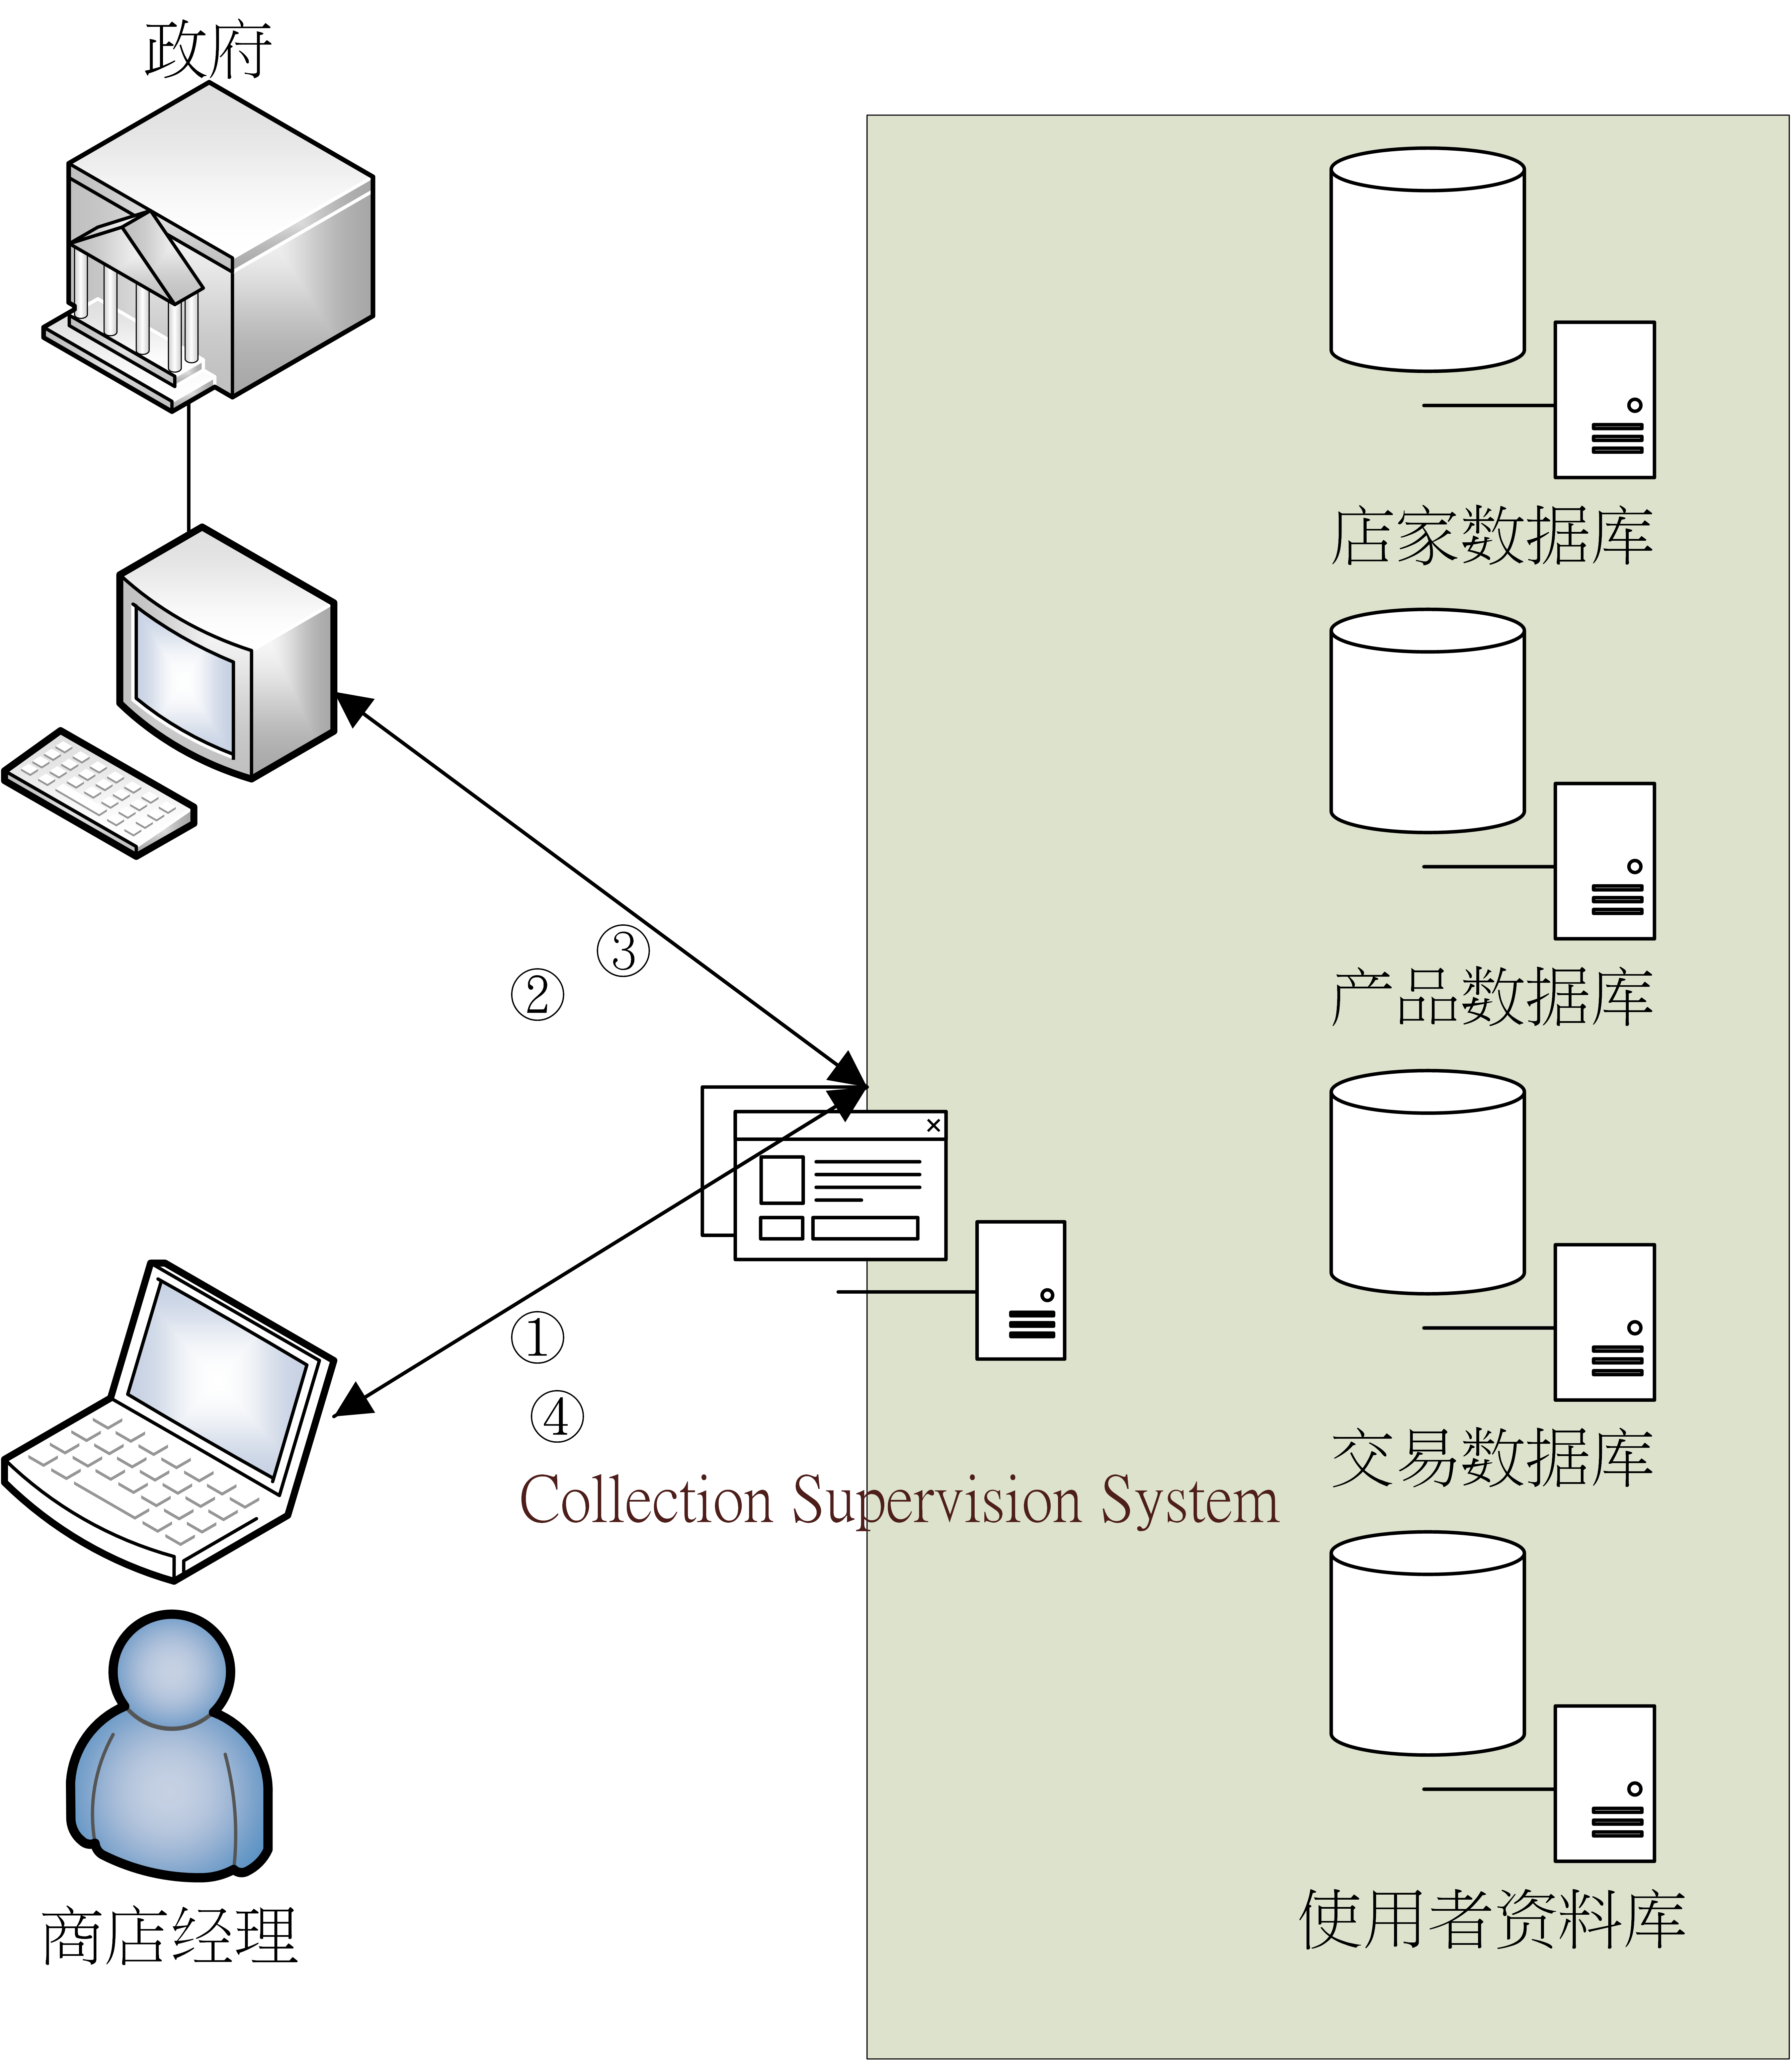
\includegraphics[width = 0.6\textwidth]{fig3.png}
		\caption{BRTMS和商家註冊流程的核心架構}\label{fig3}
	\end{figure}

	\begin{enumerate}
		\item 商戶必須在BRTMS註冊一個帳戶,並附有政府法規的商業證明。
		\item 区块链的实名交易监督系统將自動向相應的政府金融監管機構提交商業申請,以審查該商店的密碼貨幣交易業務。
		\item 如果政府批准商店的密碼貨幣業務申請,服務器將激活商家在該收集監控系統中創建商店帳戶。
		\item 商家可以自由地登錄賬戶並添加商家想要出售的產品,並檢查他們的密碼貨幣交易數據,例如產品庫存和產品交易記錄。
	\end{enumerate}

	\section{BRTMS架構與運作流程}
	具體的密碼貨幣的商家收銀金流監控系統運行過程如圖\ref{fig4}所示,我們以圖\ref{fig3}所設計出的系統架構進行擴增,首先我們需要與blockchain explorer 對接,而之所以該監控系統需要與區塊鏈檢視器對接是為了能夠最直接的比對交易被記錄的成交狀況,能夠達到即時性以及正確性,倘若擔憂單方面的依賴相信區塊鏈檢視器的成果,亦可以使用多家區塊鏈檢視器進行交叉參考,以避免因為一家公司的錯誤所帶來的影響。與區塊鏈檢視器的目的是為了能夠快速地準確地比對該筆交易的成交,做為整筆交易提出到結算的環節之一。

	\begin{figure}[h]
		\centering
		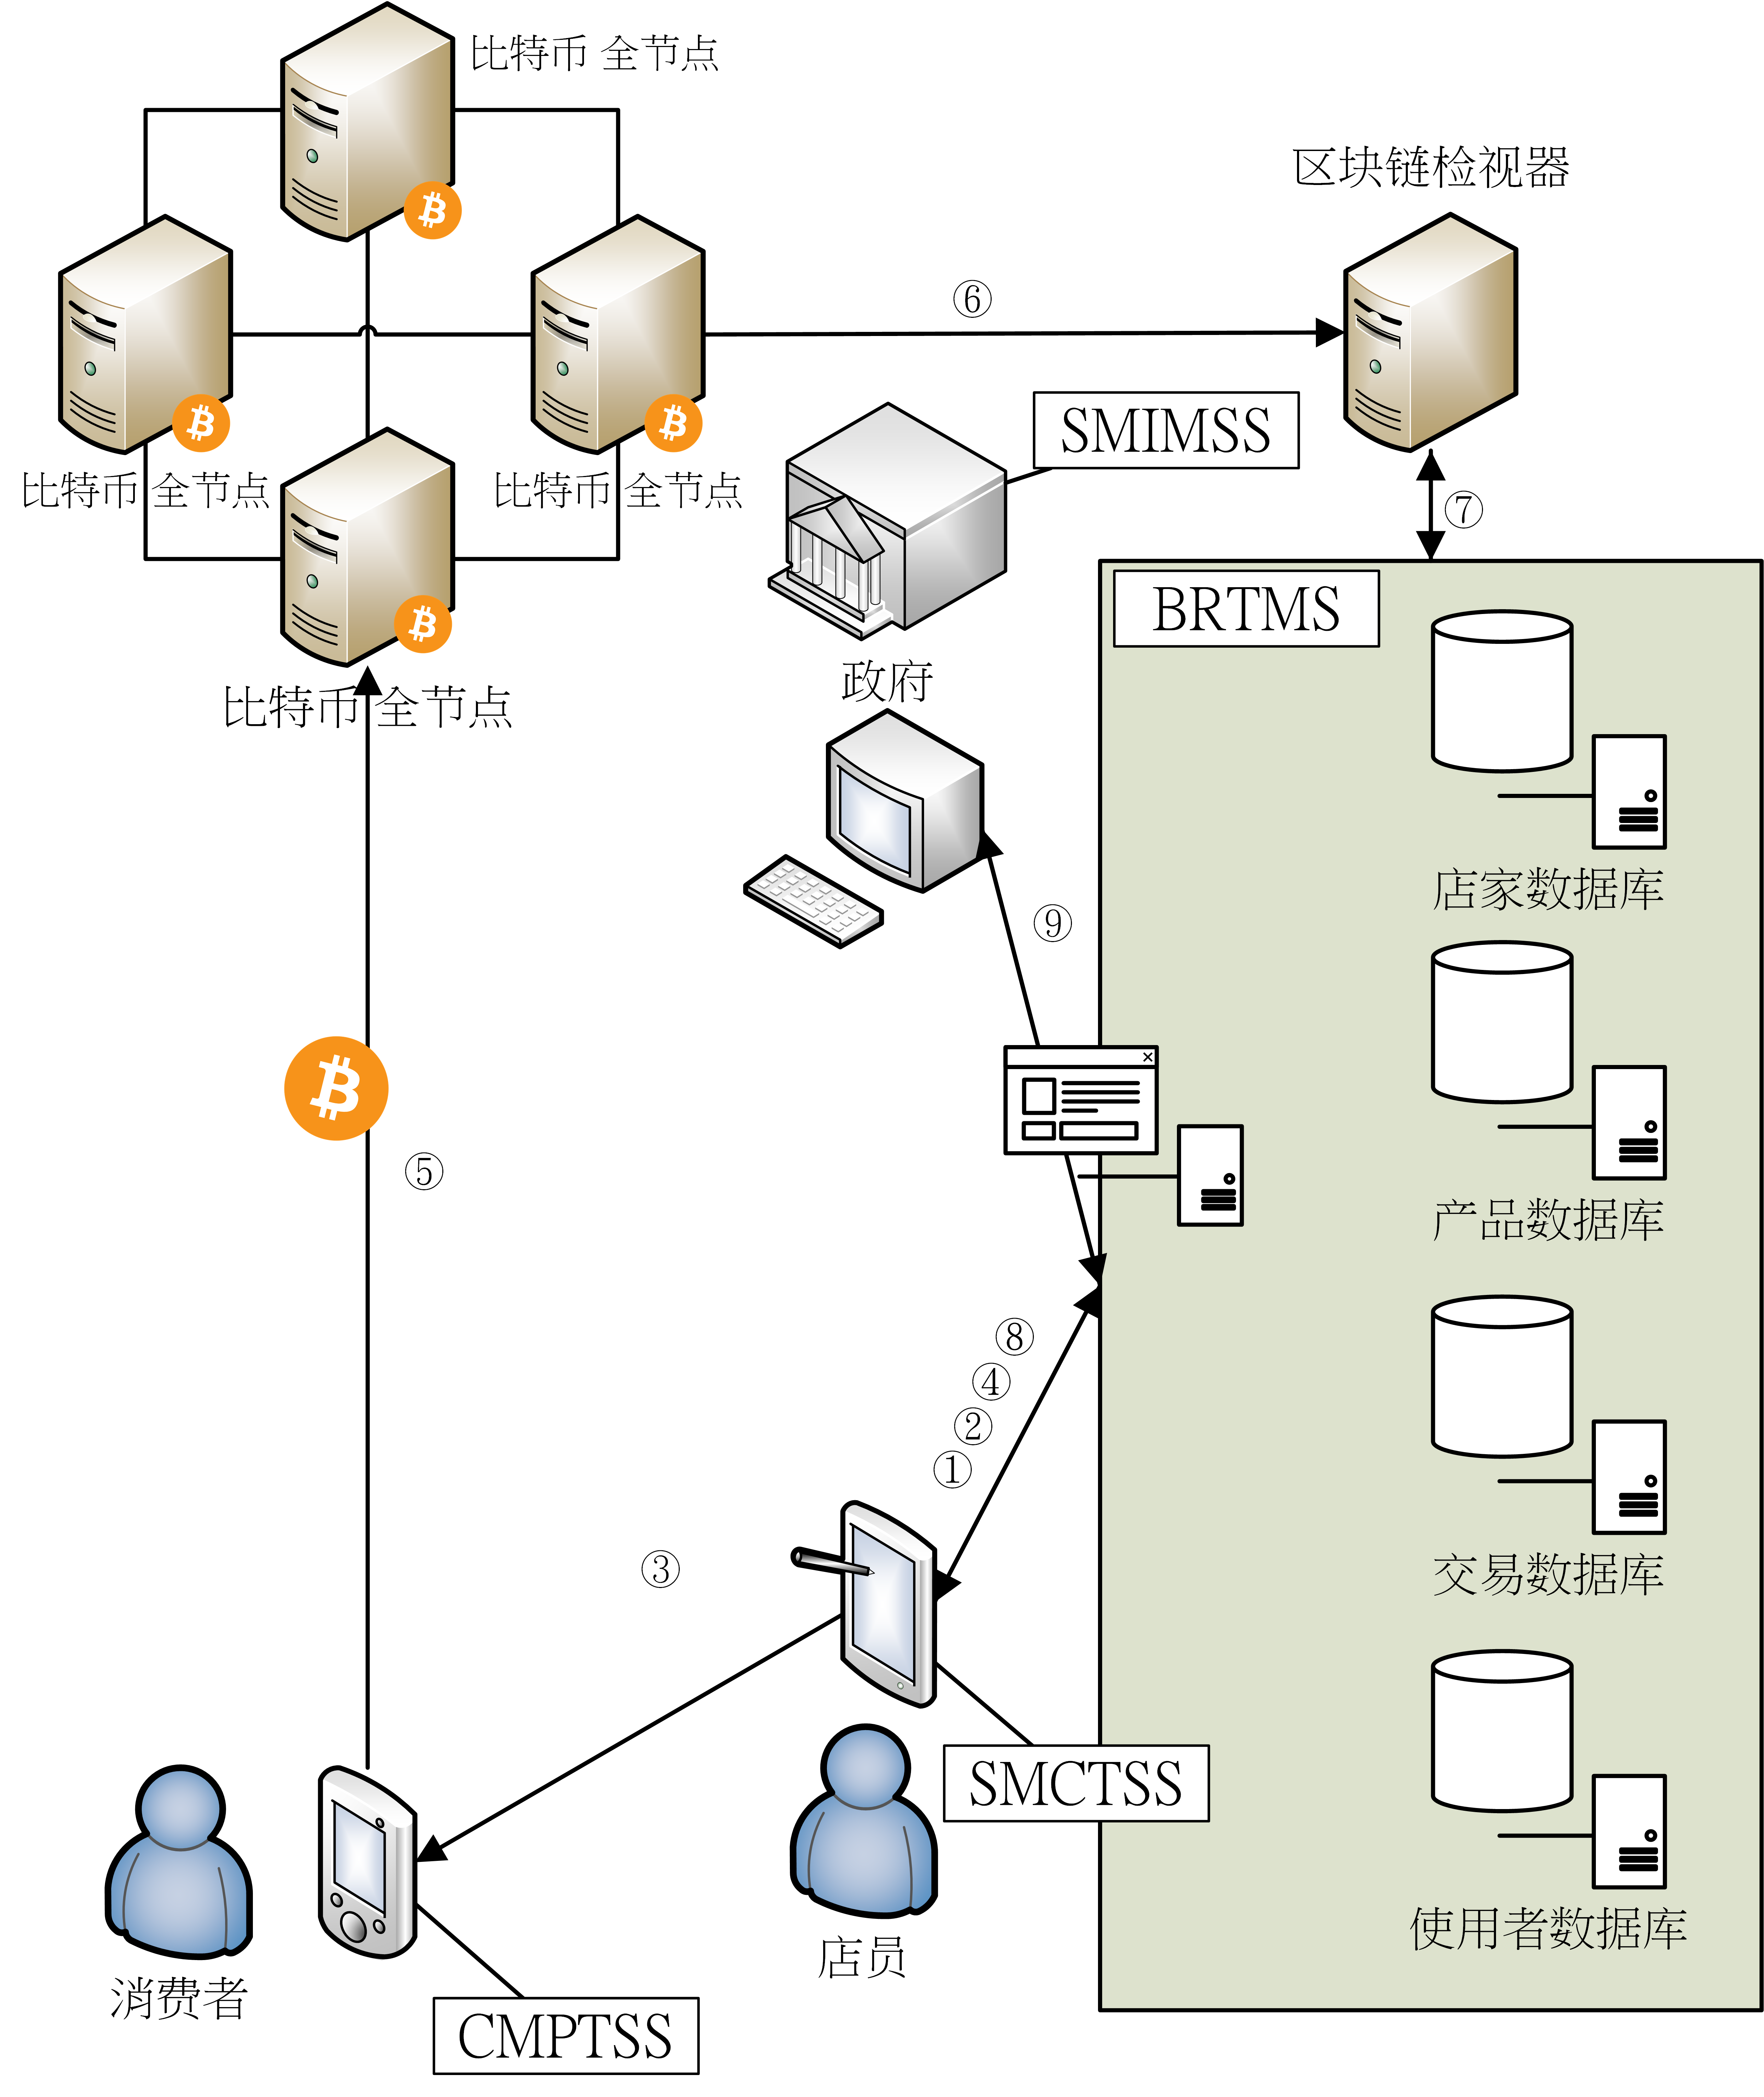
\includegraphics[width = 0.8\textwidth]{fig4.png}
		\caption{BRTMS的整體運作流程}\label{fig4}
	\end{figure}

	区块链的实名交易监督系统中創建步驟描述如下:

		\begin{enumerate}
			\item 商家的店員將登錄到如圖\ref{fig3}所示的先前步驟創建的帳戶,以使用手持式平板電腦或智能手機訪問SMCTSS中的服務。如前所述,在能夠登錄到系統之前,商家帳戶必須由政府機構審計。
			\item 在成功登錄SMCTSS用於商戶密碼貨幣流量監控系統時,移動設備將加載通過SMIMSS註冊的商店產品信息,然後創建產品目錄。商店的店員可以根據客戶的需求選擇所需的產品和數量。
			\item 店員使用設備完成客戶選定商品的產品信息後。移動設備上的NFC技術可用於將產品信息從附近店員的移動設備傳遞給消費者的移動設備,而無需物理交互。然後,消費者可以很容易地將自己的消費信息記錄為發票等參考。在接收從商家店員設備向顧客設備購買產品的消息的同時,顧客設備還將向商家的移動設備發送其自己的比特幣支付地址的消息。
			\item 商家的手持設備收到客戶確認購買所選產品的相應信息後,會將交易信息的副本發送給SMIMSS監控系統。消費者信息包括交易序列號,商戶ID號碼,商品號碼,購買的商品的數量,以及密碼貨幣的收款人地址以及消費者的支付地址。
			\item 收到消費者交易信息後,此確認將支持以比特幣等密碼貨幣支付。同時,此次交易的密碼貨幣將發佈到比特幣網絡中進行驗證和記錄。
			\item 區塊鏈瀏覽器將開始分析在比特幣網絡中緩存的所有交易以及區塊鏈中記錄的交易。
			\item 擬議的交易監控系統BRTMS將向區塊鏈檢視器提出請求。這個請求數據不僅包括存儲在BRTMS中的交易副本的密碼貨幣收款人地址(如圖\ref{fig3}的第4步所述),還包括客戶預期付款的密碼貨幣支付地址。區塊鏈瀏覽器使用請求數據來檢查交易是否存儲在區塊鏈中,或者交易還在等待確認。如果交易已被確認並存儲在區塊鏈中,則交易數據庫中“交易確認”字段的值將更改為“1”,否則其默認值為"0"。
			\item 當“交易確認”字段中的值為“1”時,“交易已完成”消息可發送至商店平板電腦上運行的商店和商品信息管理子系統(SMCTSS)。
			\item 政府財政監督部門可以審查擬議BRTMS中的所有交易信息,以作為稅收審計參考。
		\end{enumerate}
	% Copyright (c) 2014,2016 Casper Ti. Vect
\chapter{系統詳細設計與實現}
在前章中已將本文的系統設計概要架構說明,在本章中將對數據庫的內容信息設計進行詳細的說明、數據庫ER模型架構、各個模塊的類與類之間的關係、每個模塊運作的順序以及模塊與模塊之間的響應關係,最後則是系統實現的平台展示。

	\section{BTMS數據庫設計}

	比特幣的交易監督系統應用了六個信息表,分別為商家信息、產品信息、交易信息、用戶信息、職工信息以及商家產品信息,以下將逐一說明:

		\begin{figure}[!htbp]
			\centering
			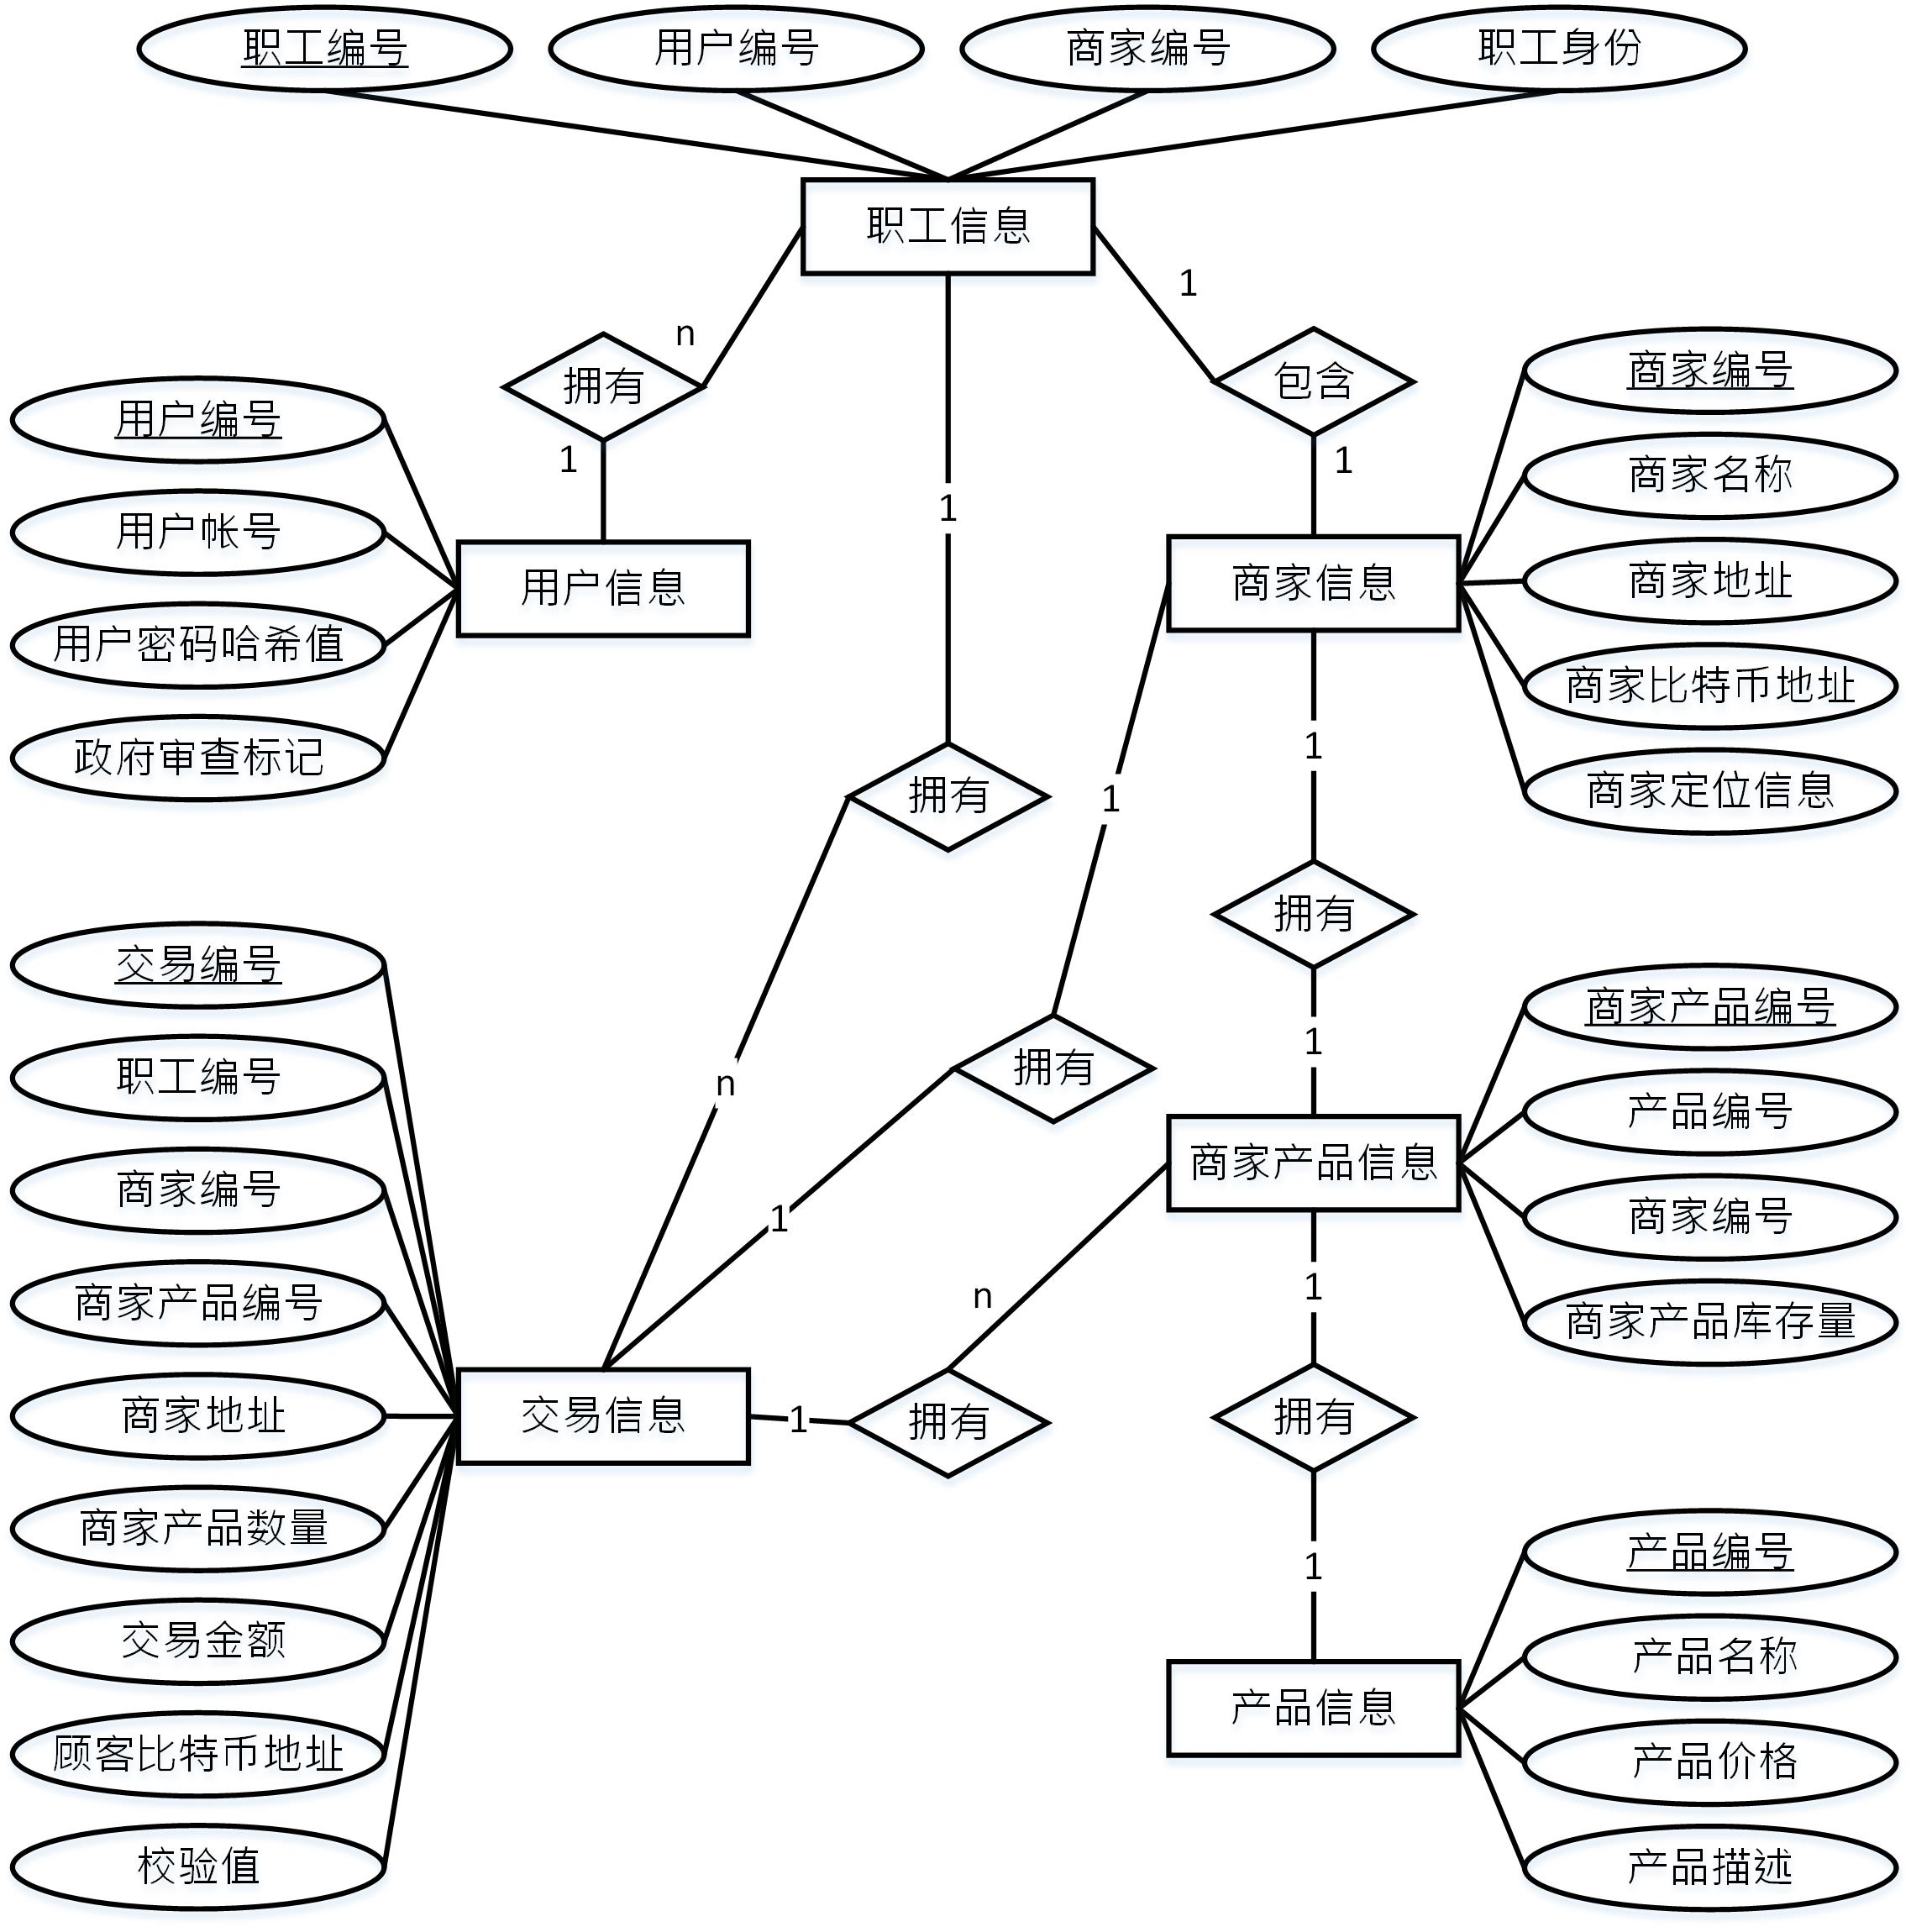
\includegraphics[width = 0.9\textwidth]{er.jpg}
			\caption{BTMS數據庫實體關係圖}\label{db}
		\end{figure}

		\begin{enumerate}
		\item 商家信息表:存儲正在審核中的企業信息或已經過審核的企業信息。表\ref{store}存儲的信息包括商家編號、商家名稱、商家地址、商家比特幣地址以及商家定位信息。


				\begin{table}[!htbp]
				\centering
				\caption{商家信息表}
				\label{store}
				\resizebox{\textwidth}{!}{%
				\begin{tabular}{|c|c|c|c|c|c|}
				\hline
				序號 & 字段名 & 字段說明 & 類型 & 是否為空 & 主外鍵 \\ \hline
				1 & STORE\_ID & 商家編號 & int & 否 & PK \\ \hline
				2 & STORE\_NAME & 商家名稱 & navarchar(20) & 否 &  \\ \hline
				3 & STORE\_ADDRESS & 商家地址 & navarchar(50) & 否 &  \\ \hline
				4 & STORE\_BTCADDRESS & 商家比特幣地址 & navarchar(50) & 否 &  \\ \hline
				5 & STORE\_GPS & 商家定位信息 & navarchar(30) & 否 &  \\ \hline
				\end{tabular}%
				}
				\end{table}

		\item 產品信息表:只有授權用戶才能登錄添加或修改交易產品信息。表\ref{product}產品信息表內容包括產品編號、產品名稱、產品價格以及產品描述信息。

				\begin{table}[!htbp]
				\centering
				\caption{產品信息表}
				\label{product}
				
				\begin{tabular}{|c|c|c|c|c|c|}
				\hline
				序號 & 字段名 & 字段說明 & 類型 & 是否為空 & 主外鍵 \\ \hline
				1 & PRODUCT\_ID & 產品編號 & int & 否 & PK \\ \hline
				2 & PRODUCT\_NAME & 產品名稱 & navarchar(10) & 否 &  \\ \hline
				3 & PRODUCT\_PRICE & 產品價格 & float & 否 &  \\ \hline
				4 & PRODUCT\_DESCRIPTION & 產品描述 & navarchar(50) & 是 &  \\ \hline
				\end{tabular}
				\end{table}

		\item 交易信息表:表\ref{tx}記錄包括交易編號、職工編號、商家編號、商家產品編號、商家地址、商家產品數量、交易金額、顧客比特幣地址和最後確認字段的校驗值。

				% \usepackage{graphicx}
				\begin{table}[!htbp]
				\centering
				\caption{交易信息表}
				\label{tx}
				\resizebox{\textwidth}{!}{%
				\begin{tabular}{|c|c|c|c|c|c|}
				\hline
				序號 & 字段名 & 字段說明 & 類型 & 是否為空 & 主外鍵 \\ \hline
				1 & TX\_ID & 交易編號 & int & 否 & PK \\ \hline
				2 & STAFF\_ID & 職工編號 & int & 否 & FK \\ \hline
				3 & STORE\_ID & 商家編號 & int & 否 & FK \\ \hline
				4 & STOREPRODUCT\_ID & 商家產品編號 & int & 否 & FK \\ \hline
				5 & STORE\_ADDRESS & 商家地址 & navarchar(50) & 否 & FK \\ \hline
				6 & STOREPRODUCT\_QUANTITY & 商家產品數量 & int & 否 &  \\ \hline
				7 & TX\_AMOUNT & 交易金額 & float & 否 &  \\ \hline
				8 & CONSUMER\_BTCADDRESS & 顧客比特幣地址 & navarchar(50) & 否 &  \\ \hline
				9 & CHECK & 校驗值 & bool & 否 &  \\ \hline
				\end{tabular}%
				}
				\end{table}

		\item 用戶信息表:表\ref{user}存儲所有用戶信息,包括政府、商家及顧客之個人的帳戶編號與帳號,而用戶密碼則以哈希值的方式保存以增加用戶安全性,最後則是政府審查值,倘若通過為"1",未通過為"0"。

				\begin{table}[!htbp]
				\centering
				\caption{用戶信息表}
				\label{user}
				\resizebox{\textwidth}{!}{%
				\begin{tabular}{|c|c|c|c|c|c|}
				\hline
				序號 & 字段名 & 字段說明 & 類型 & 是否為空 & 主外鍵 \\ \hline
				1 & USER\_ID & 用戶編號 & int & 否 & PK \\ \hline
				2 & USER\_ACCOUNT & 用戶帳號 & navarchar(30) & 否 &  \\ \hline
				3 & USER\_PASSWORDHASH & 用戶密碼哈希值 & navarchar(30) & 否 &  \\ \hline
				4 & GOVT\_AUTH & 政府審查 & bool & 否 &  \\ \hline
				\end{tabular}
				}
				\end{table}

		\item 職工信息表:表\ref{staff}信息表存儲各個商家擁有的職工信息,包括各職工編號、用戶編號、商家編號及職工身份。
				\begin{table}[!htbp]
				\centering
				\caption{職工信息表}
				\label{staff}
				\begin{tabular}{|c|c|c|c|c|c|}
				\hline
				序號 & 字段名 & 字段說明 & 類型 & 是否為空 & 主外鍵 \\ \hline
				1 & STAFF\_ID & 職工編號 & int & 否 & PK \\ \hline
				2 & USER\_ID & 用戶編號 & int & 否 & FK \\ \hline
				3 & STORE\_ID & 商家編號 & int & 否 & FK \\ \hline
				4 & STAFF\_STATUS & 職工身份 & navarchar(20) & 否 &  \\ \hline
				\end{tabular}
				\end{table}

		\item 商家產品信息表:表\ref{storeproduct}存儲各家商家當前商家產品存貨信息,由商家產品編號、產品編號、商家編號及商家產品庫存量所組成。
				\begin{table}[!htbp]
				\centering
				\caption{商家產品信息表}
				\label{storeproduct}
				\begin{tabular}{|c|c|c|c|c|c|}
				\hline
				序號 & 字段名 & 字段說明 & 類型 & 是否為空 & 主外鍵 \\ \hline
				1 & STOREPRODUCT\_ID & 商家產品編號 & int & 否 & PK \\ \hline
				2 & PRODUCT\_ID & 產品編號 & int & 否 & FK \\ \hline
				3 & STORE\_ID & 商家編號 & int & 否 & FK \\ \hline
				4 & STOREPRODUCT\_INVENTORY & 商家產品庫存量 & int & 否 &  \\ \hline
				\end{tabular}
				\end{table}

	\end{enumerate}

\section{系統模塊設計}
在本系統中共有三種用戶,分別為顧客、商家以及職工,首先是用戶註冊與登入模塊,其餘總共有四個管理模塊分別為商家產品管理模塊、職工管理模塊、商家交易管理模塊和顧客交易管理模塊,以下將說明各個模塊類圖設計以及時序圖運作。

\subsubsection{(一)用戶註冊與登入模塊}
在本系統中僅職工與商家需要進行註冊,並且需要經過政府的審查批准。職工與商家皆為用戶,皆可使用用戶註冊模塊。圖\ref{c3}為用戶註冊與登入模塊類圖,在LoginManagement類當中分別需要調用RegistNewUser類實現用戶註冊以及LoginUser類實現用戶登入。RegistNewUser類中hash()方法是將用戶輸入的用戶密碼使用哈希算法生成用戶密碼哈希值,addnewuser()方法則是將用戶帳號和密碼傳送至User類。在LoginUser類中getuserpasswordhash()方法是向User類取得該用戶帳號的密碼哈希值。

	\begin{figure}[!htbp]
		\centering
		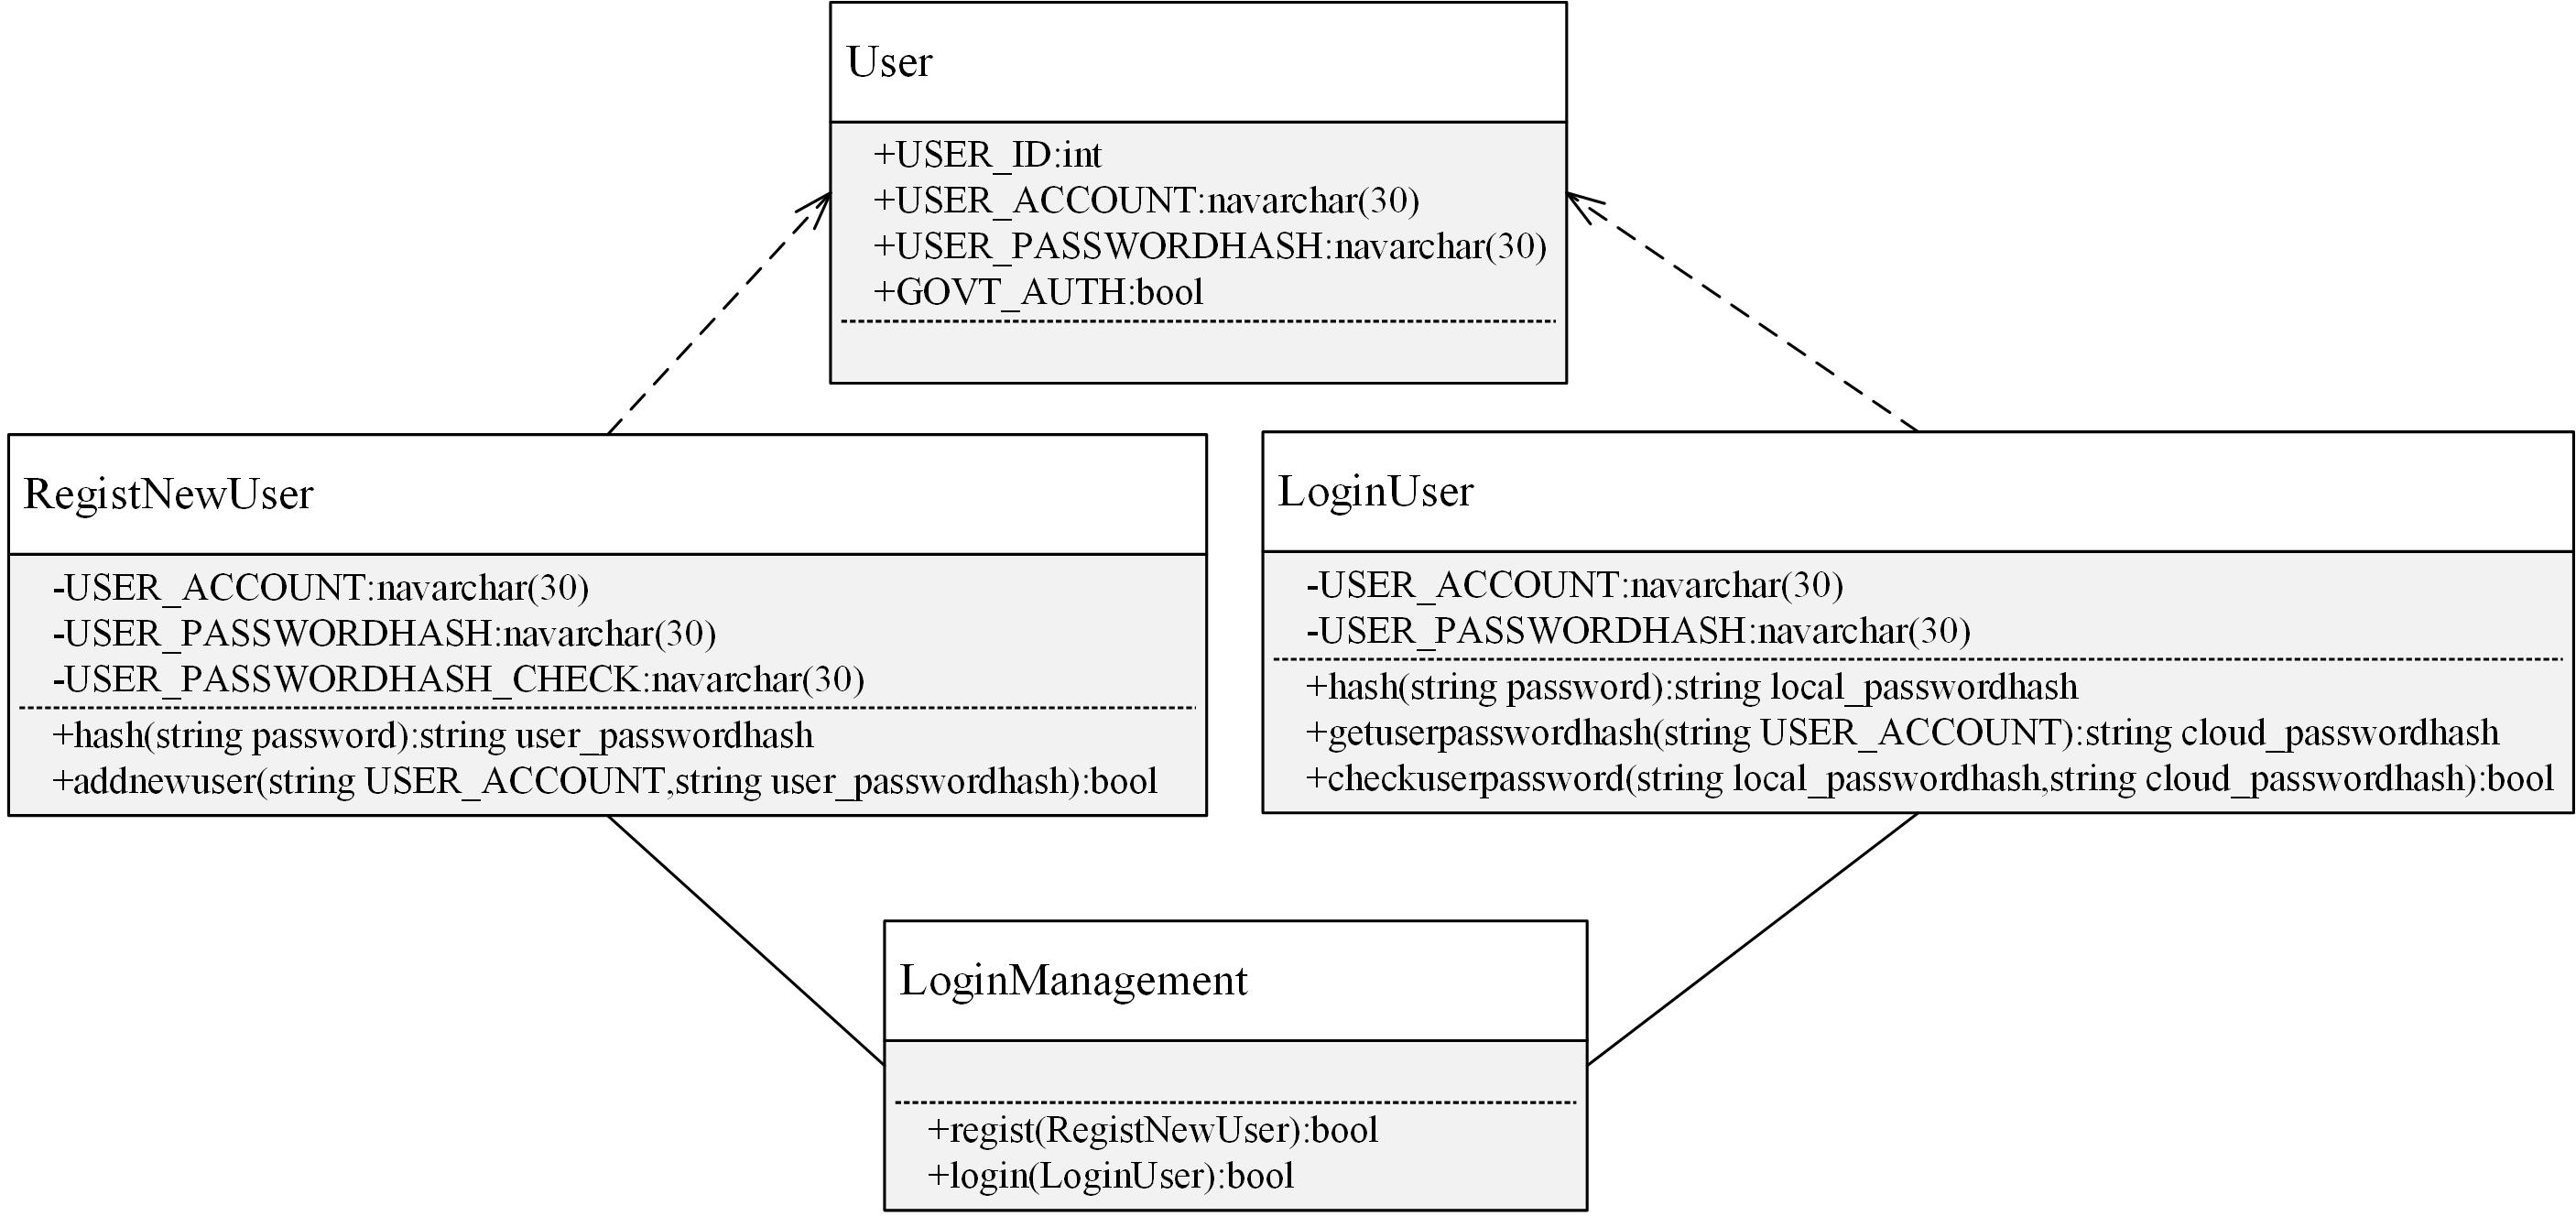
\includegraphics[width = 1\textwidth]{c3.jpg}
		\caption{用戶註冊與登入模塊類圖}\label{c3}
	\end{figure}

	圖\ref{time1}為職工與商家註冊時序圖,以下為流程說明:

	\begin{figure}[!htbp]
		\centering
		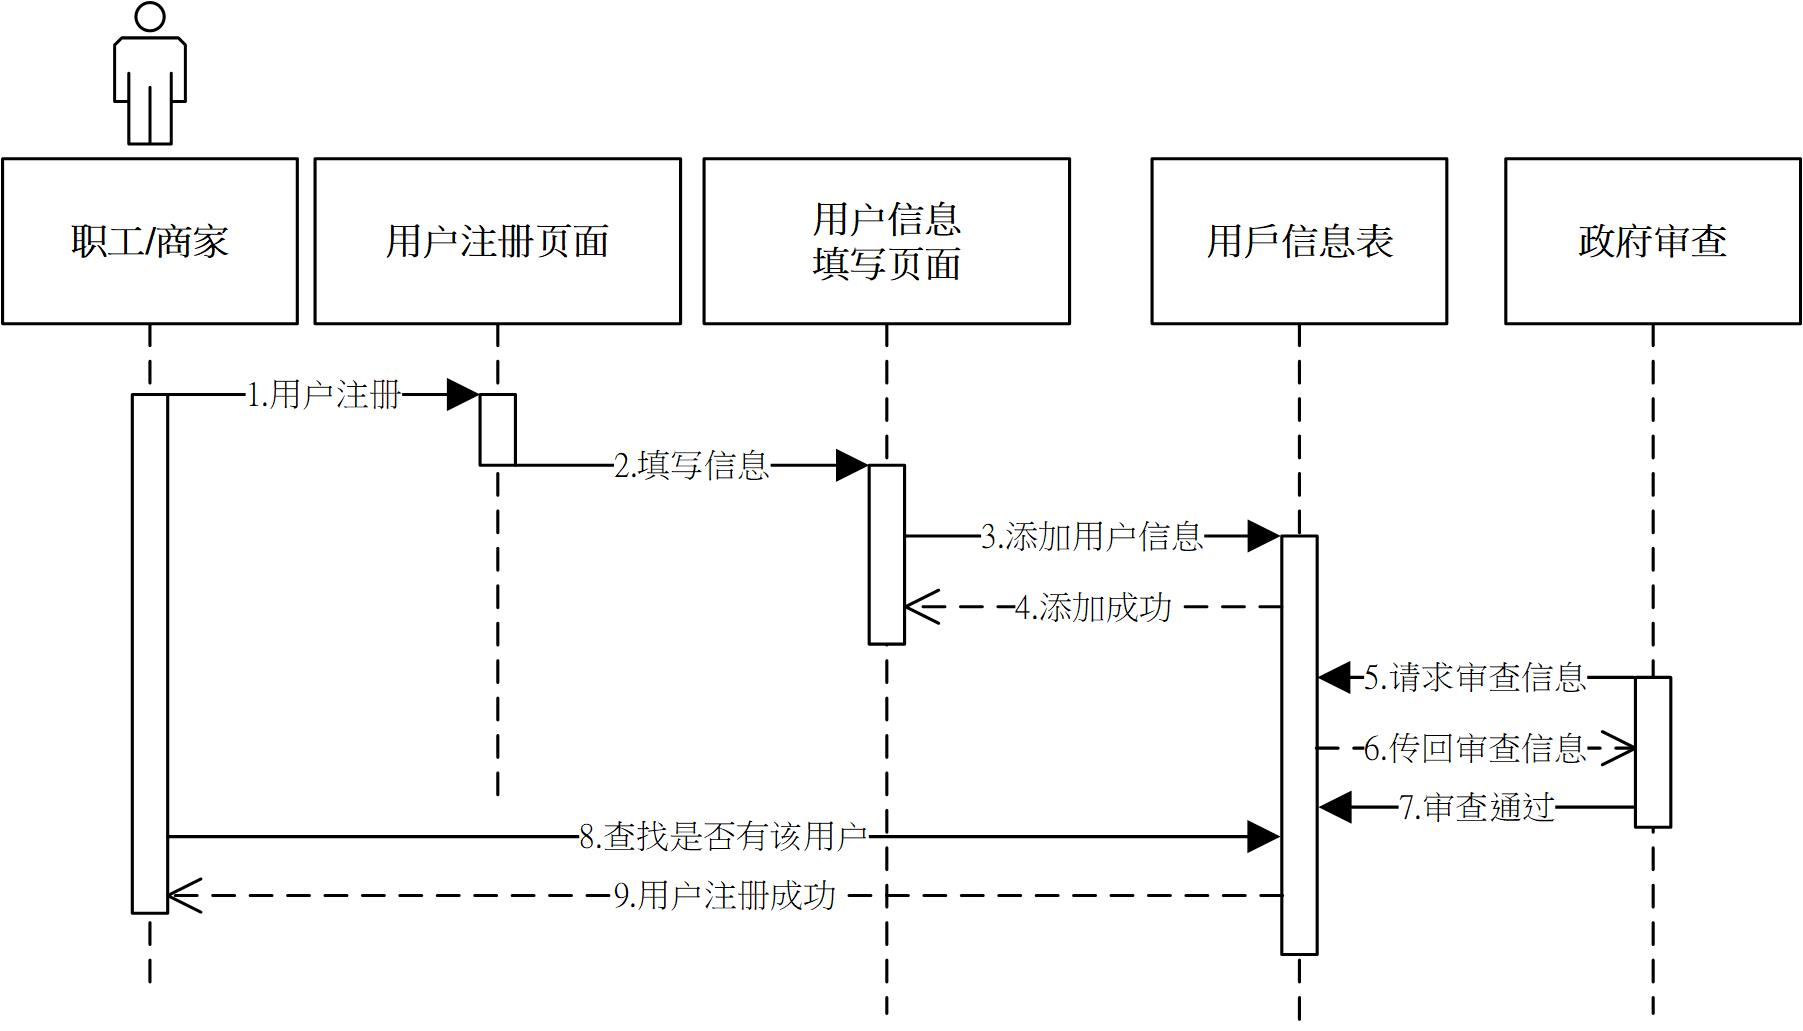
\includegraphics[width = 0.9\textwidth]{time1.jpg}
		\caption{職工與商家註冊時序圖}\label{time1}
	\end{figure}

	\begin{enumerate}
	\item 首先職工或是商家前往用戶註冊頁面。
	\item 前往用戶信息填寫頁面填寫用戶帳戶信息以及用戶密碼。
	\item 完成填寫後,為了提升用戶密碼信息安全,將用戶密碼以哈希算法計算後以密碼哈希值保存。將填寫完的帳號信息以及密碼哈希值提交到用戶信息表。
	\item 用戶信息表則傳回添加成功。屆時的用戶信息已經存儲到用戶信息表內但是尚未被激活,需要等待政府進行審查。
	\item 政府向用戶信息請求表拿取所有還未被激活的用戶信息。
	\item 數據庫中的用戶信息表傳回,政府請求的用戶信息清單。
	\item 政府進行用戶審查,在完成用戶審查後,則向用戶信息表內輸入審查通過。
	\item 此時,用戶再次訪問用戶信息表當中,用戶帳號是否已經激活成功。
	\item 用戶信息表回傳已經驗證通過。
	\end{enumerate}


\subsubsection{(二)商家產品管理模塊}
商家的運營需要管理本⾝所需販售的商品。在商家完成註冊⽤⼾帳號並且通過政府審核之後,便可檢視所有的產品,近⼀步可以透過產品管理模塊新增、修改以及刪除商家商品。圖\ref{c2}為商家產品管理類圖,其中StoreProductManagement 類中有四個⽅法需要實現,分別為顯⽰商家信息的showstoreinfo() ⽅法、顯⽰商家產品信息的showstoreproductinfo() ⽅法、顯⽰產品信息的showproductinfo() 以及修改商家產品信息的edit()⽅法。其中StoreProductCompare 類與EditStoreProduct 類需要向StoreProduct 請求商家產品信息,StoreProductCompare 類中的compare() ⽅法是向商家產品信息表取得與STORE\_ID 相符的所有相關商家產品。EditStoreProduct 類中的addstoreproduct() ⽅法、editstoreproduct() ⽅法、以及deletestoreproduct() ⽅法分別為新增、修改、以及刪除商家產品信息。StoreCompare 類中的compare() ⽅法是向Store 類請求與STORE\_ID 相符的商家信息。

	\begin{figure}[!htbp]
		\centering
		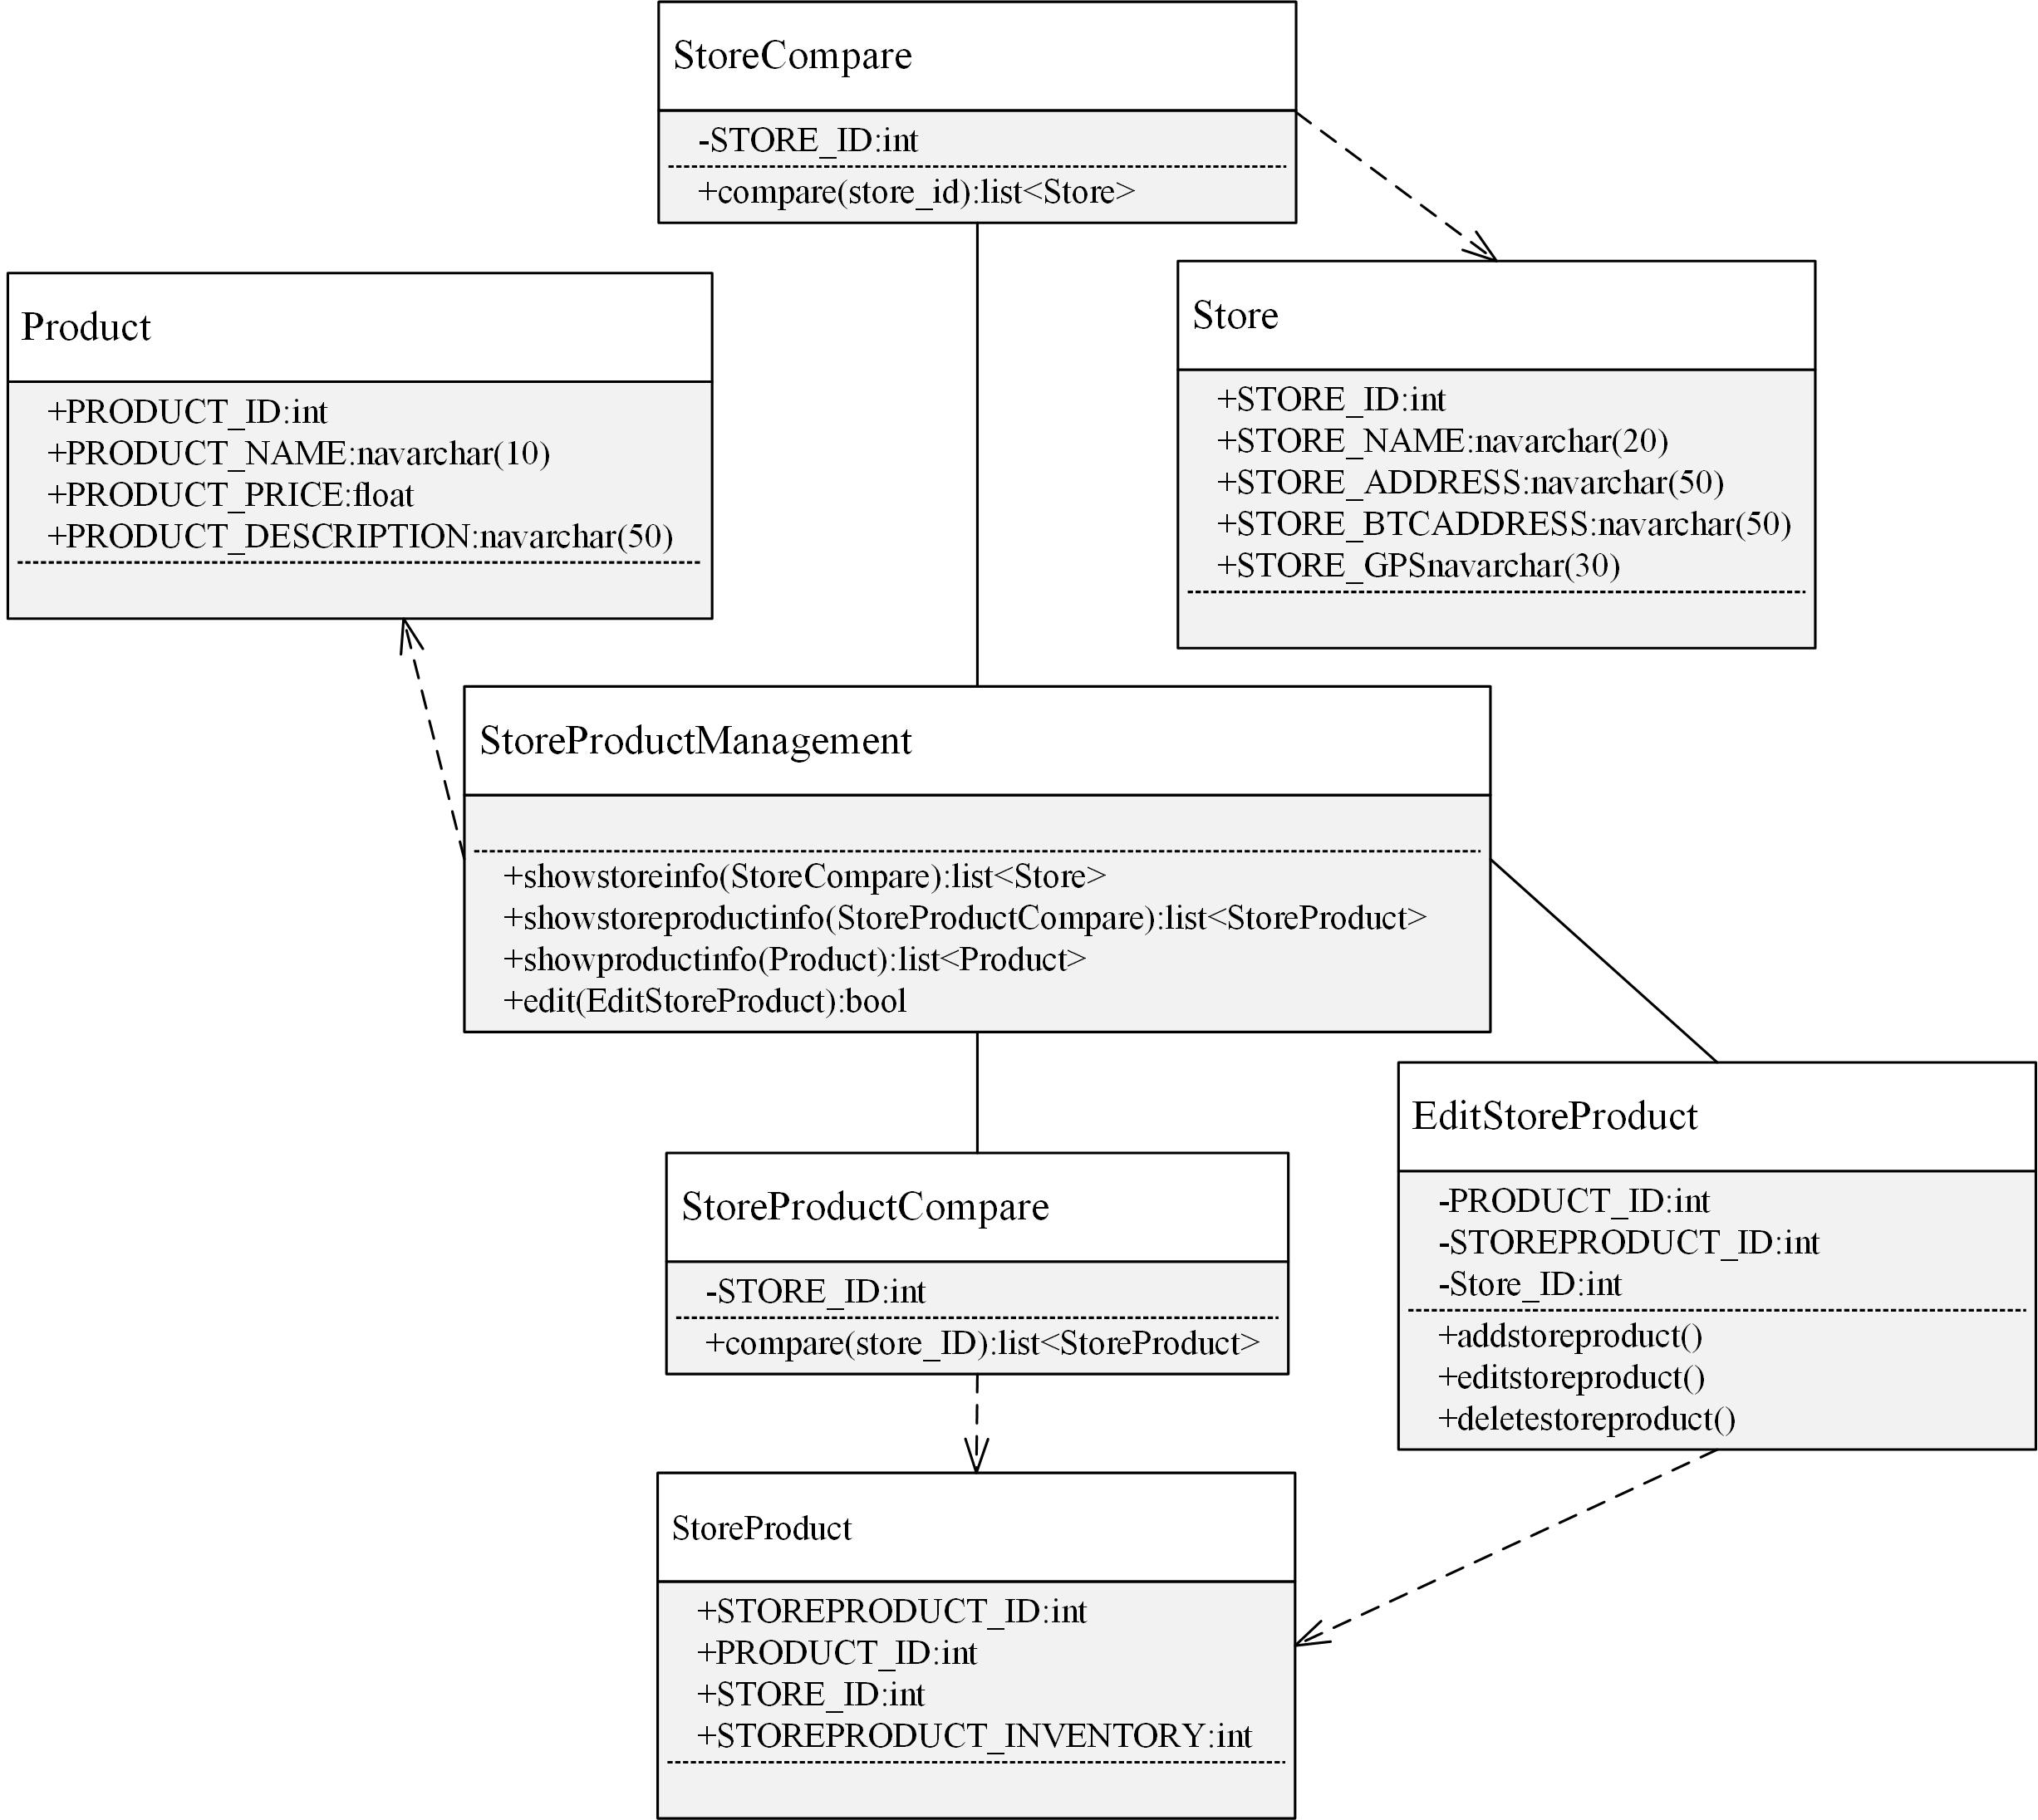
\includegraphics[width = 0.9\textwidth]{c2.jpg}
		\caption{商家產品管理類圖}\label{c2}
	\end{figure}

	圖\ref{time3}為商家產品管理時序圖,以下為流程說明:

	\begin{figure}[!htbp]
		\centering
		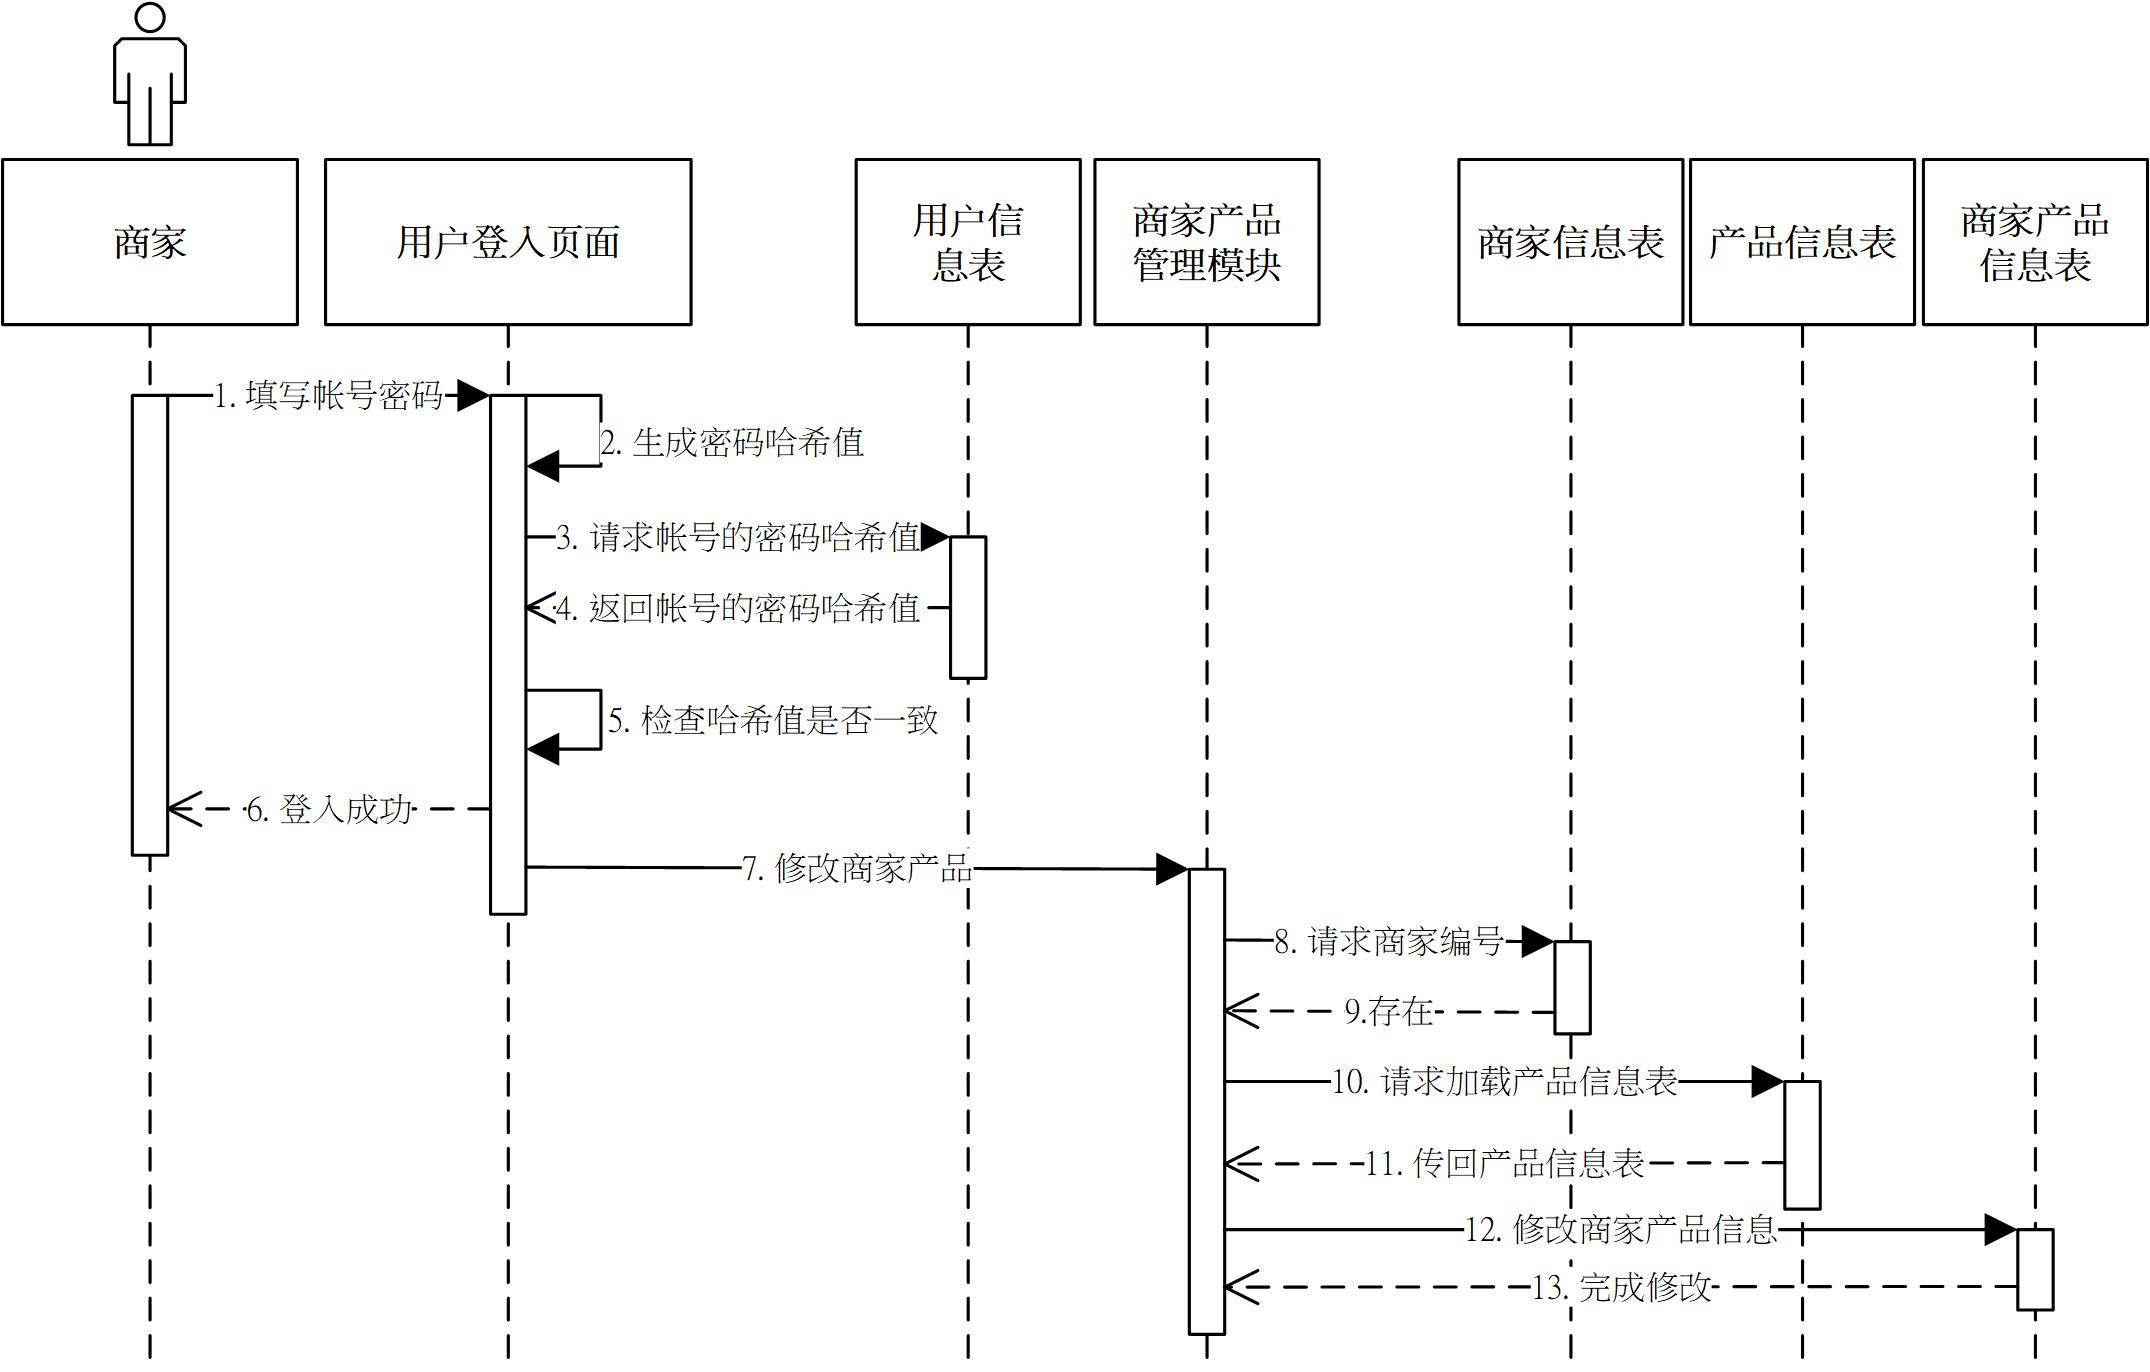
\includegraphics[width = 0.9\textwidth]{time3.jpg}
		\caption{商家產品管理時序圖}\label{time3}
	\end{figure}

	\begin{enumerate}
	\item 商家在完成用戶註冊後並完成政府的審核之後,便可填寫使用用戶與用戶密碼到登入頁面。
	\item 登入頁面會將用戶提交之密碼透過哈希算法生成密碼哈希值。
	\item 用戶登入頁面向用戶信息表詢問該用戶帳號的密碼哈希值。
	\item 用戶信息表將該帳戶的密碼哈希值傳回給用戶登入頁面保存。
	\item 用戶頁面將本地密碼哈希值和從數據庫信息表中請求保存的密碼哈希值進行比對是否相同。
	\item 倘若本地與數據庫中的哈希值一致,則為登入成功。
	\item 屆時可以進入商家產品管理模塊。
	\item 為確認欲修改的商家是否存在,所以向數據庫中的商家信息表請求該商家編號是否存在。
	\item 商家信息表返回存在的信息。
	\item 向數據庫中的產品信息表當中請求所有的產品信息。
	\item 產品信息表回傳所有的產品信息。
	\item 此時商家已經確認商家信息是否存在,且已經取得所有的產品信息。商家向商家產品信息表提交商家要增加的產品編號以及商家本身的商家編號,此時生成商家產品編號。
	\item 商家信息表在完成添加商家產品信息之後,傳回添加成功的信息到商家產品管理模塊。
	\end{enumerate}


\subsubsection{(三)職工管理模塊}
商家需要職⼯進⾏商家的運營。在商家⽤⼾完成政府審查之後,便可以進⼊職⼯管理模塊,透過提交⽤⼾編號以及商家編號新增、修改以及刪除職⼯信息。圖\ref{c1}為職⼯管理模塊類圖,StaffManagement 類當中有四種⽅法,前三種分別為顯⽰與該商家STORE\_ID 相符的完整信息showstore() ⽅法、顯⽰符合該商家STORE\_ID 職⼯信息的showstorestaff() ⽅法、顯⽰⽤⼾編號的showuser() ⽅法。而在第四種方法中,UserCompare 類需要向User 類提取⽤⼾相關信息實現查詢,StoreCompare 類需要向Store 類請求商家信相關信息,其中EditStoreStaff 類與StoreStaffCompare 類需要使⽤到Staff 類修改職⼯信息表的內容,EditStoreStaff 類中的addstaff()、editstaff() 以及deletestaff() ⽅法分別為新增、修改以及刪除職⼯,StoreStaffCompare 類中的compare ⽅法是取得符合STORE\_ID 的所有職⼯信息。

	\begin{figure}[!htbp]
		\centering
		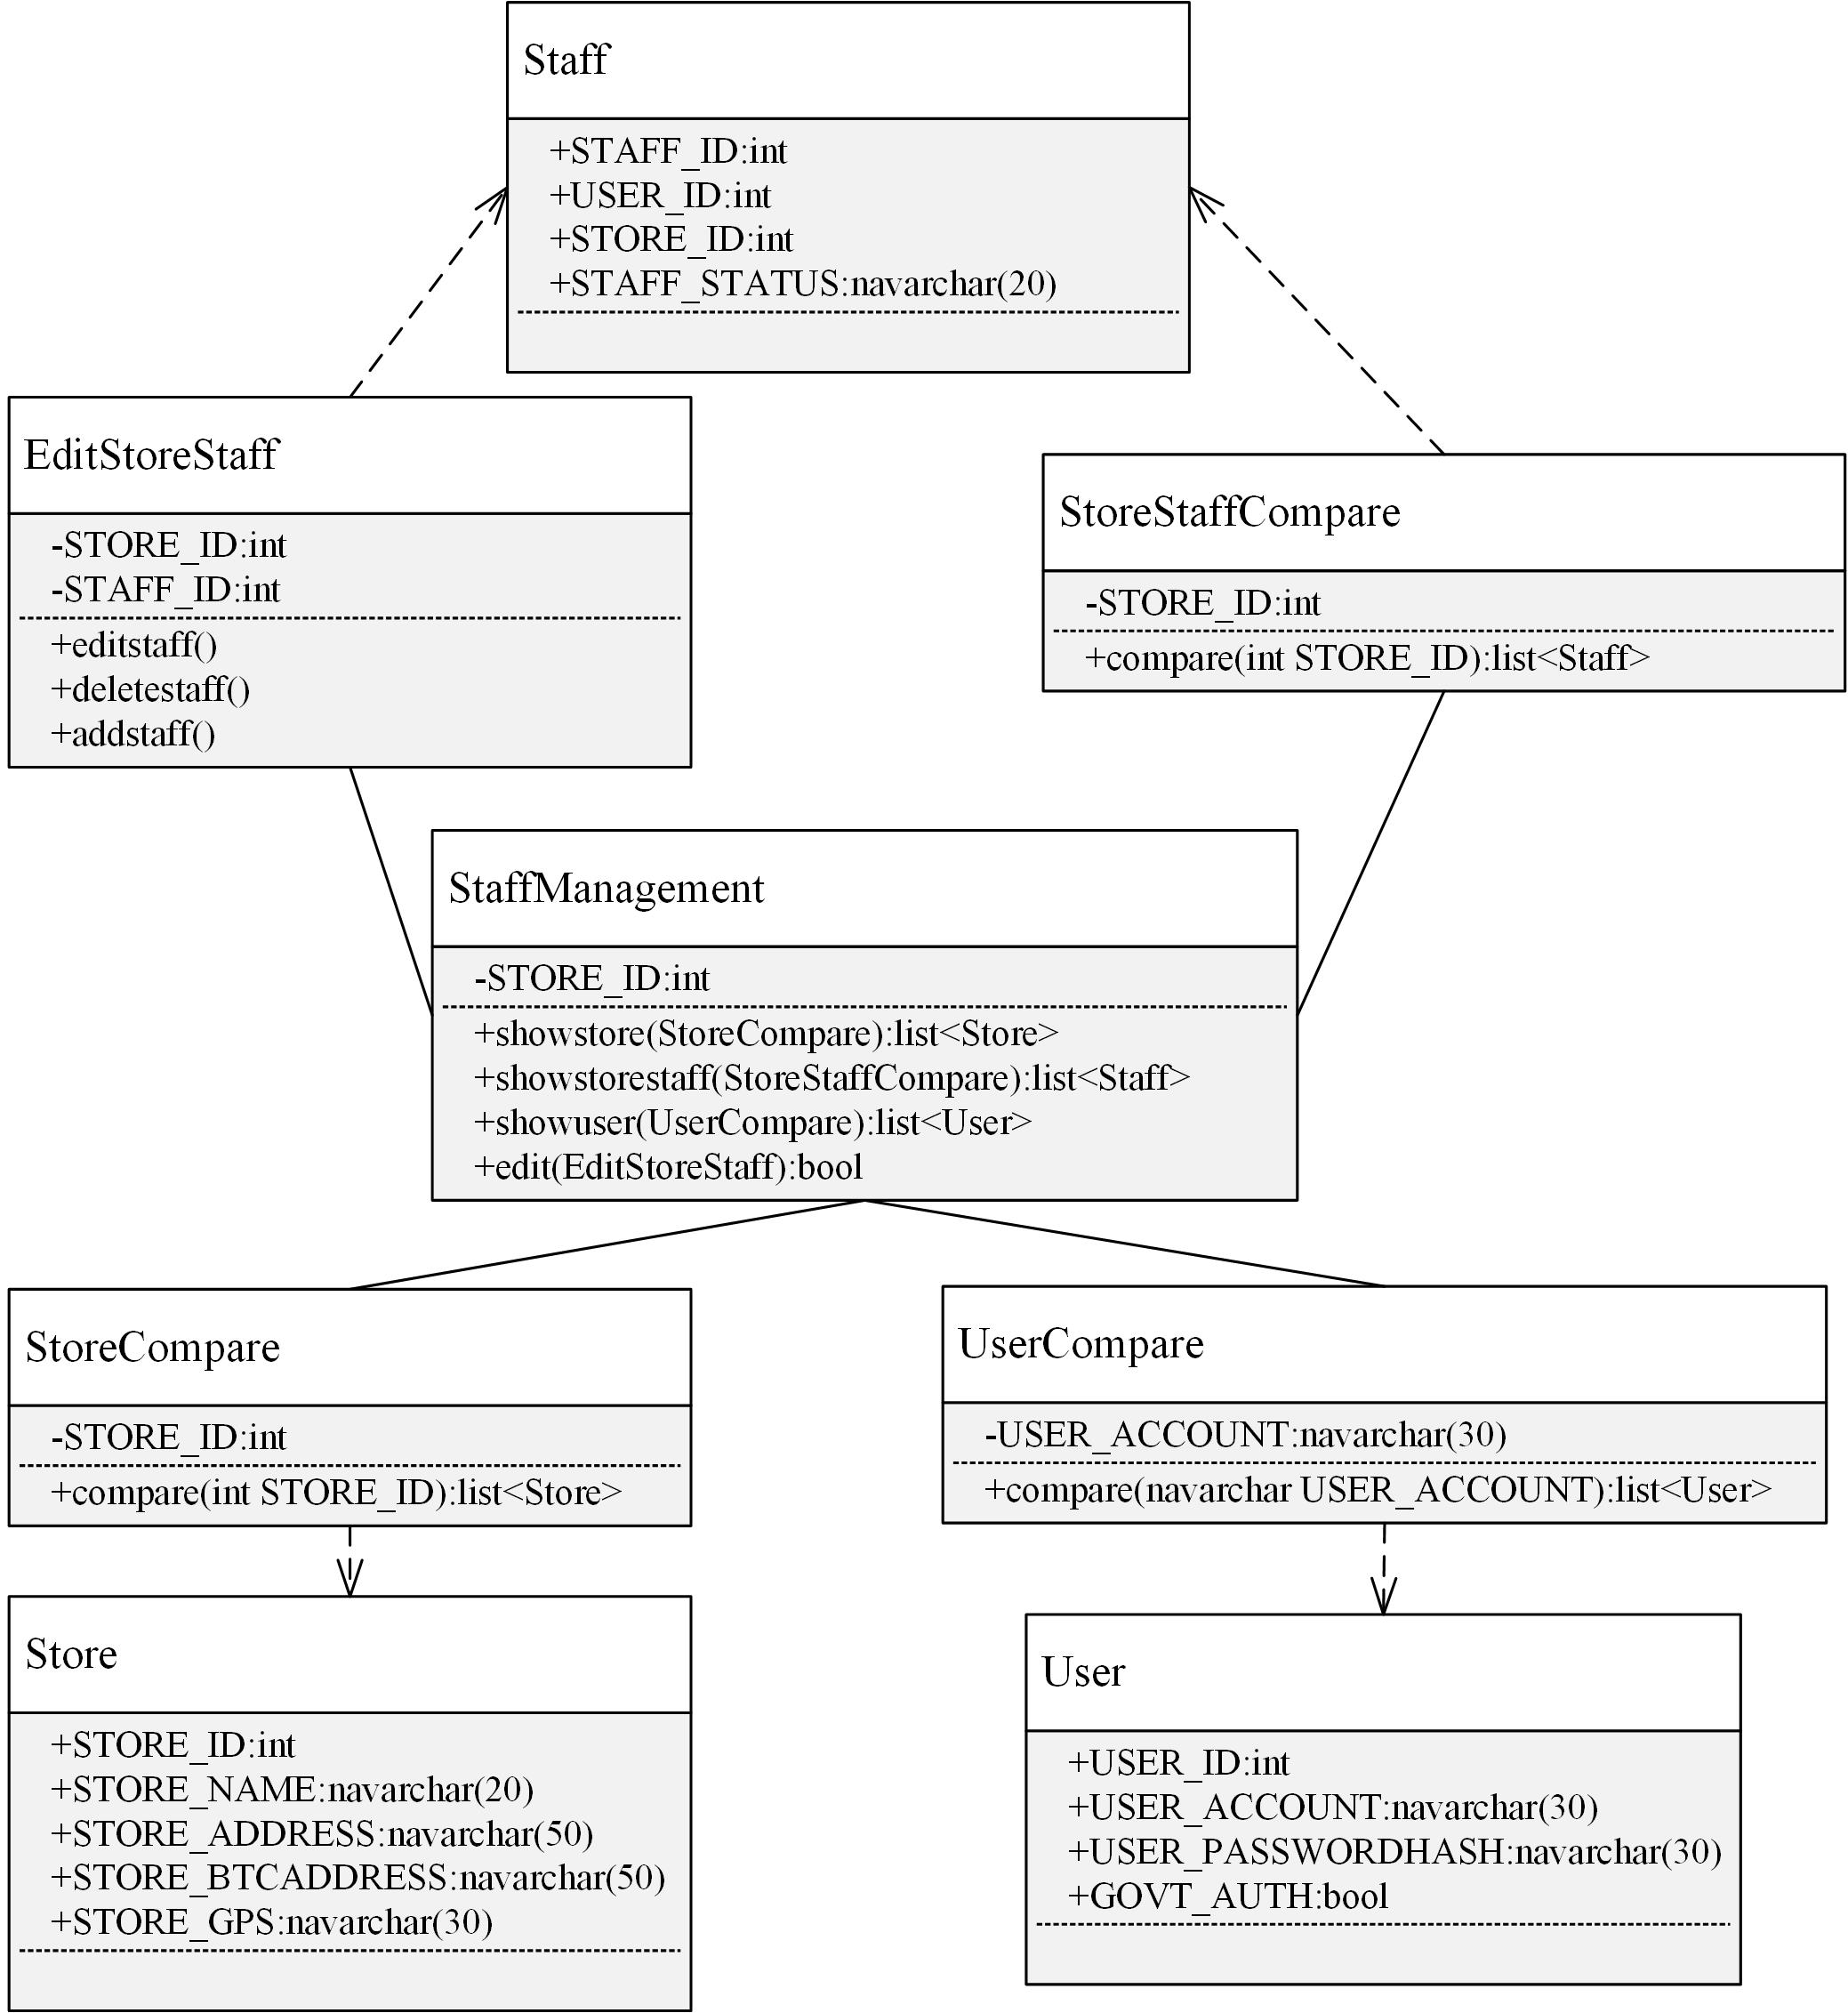
\includegraphics[width = 0.8\textwidth]{c1.jpg}
		\caption{職工管理模塊類圖}\label{c1}
	\end{figure}

	

	圖\ref{time2}為商家職工管理時序圖,以下為流程說明:

	\begin{figure}[!htbp]
		\centering
		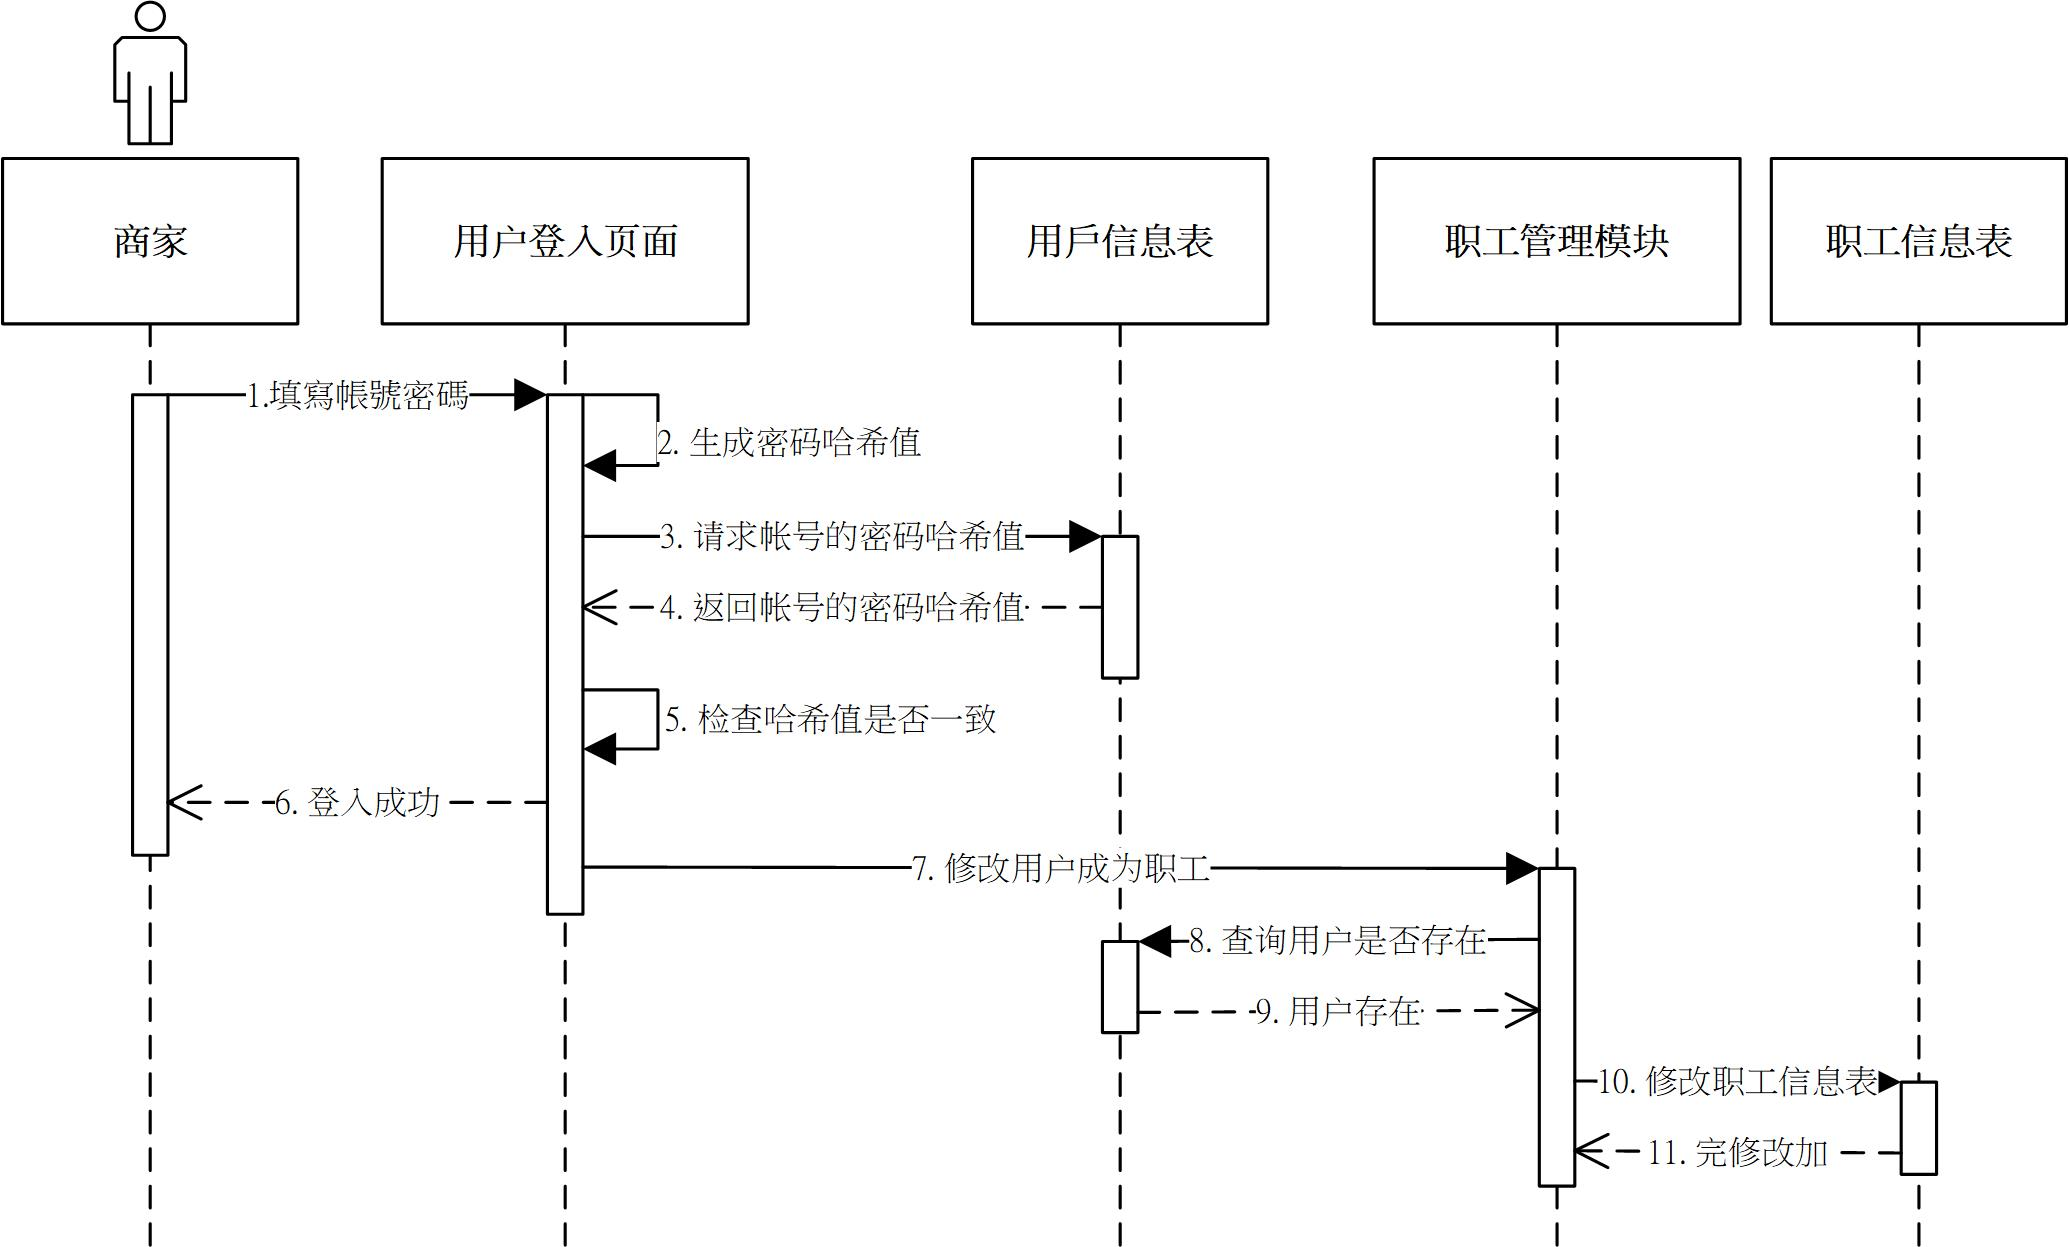
\includegraphics[width = 0.9\textwidth]{time2.jpg}
		\caption{商家職工管理時序圖}\label{time2}
	\end{figure}

	\begin{enumerate}
	\item 商家前往用戶登入頁面輸入用戶帳號密碼。
	\item 用戶登入頁面自動使用哈希算法將用戶密碼轉換成密碼哈希值。
	\item 用戶登入頁面向數據庫中的用戶信息表請求該用戶帳號的密碼哈希值。
	\item 數據庫用戶信息表回傳用戶密碼哈希值。
	\item 用戶登入頁面比對本地端的用戶密碼哈希值與數據庫中的密碼哈希值是否一致。
	\item 倘若數據庫中的密碼哈希值與用戶登入頁面生成的密碼哈希值一致,則登入成功。
	\item 商家提交商家編號以及欲添加的用戶編號。
	\item 職工管理模塊向用戶信息表查詢該用戶是否存在。
	\item 用戶信息表傳回用戶存在信息。
	\item 職工管理模塊向數據庫中的職工信息表提交用戶編號、商家編號以及職工編號修改職工信息。
	\item 職工信息表傳回修改完成。
	\end{enumerate}

\subsubsection{(四)商家交易管理模塊}
在⽤⼾完成註冊後且在商家將該⽤⼾加⼊成為公司職⼯後,該職⼯可以透過⽤⼾帳號進⼊到商家交易管理模塊,該模塊為移動裝置的應⽤程序。在進⼊到本模塊後會⾃動加載商家商品、商家信息以及職⼯信息,製成⼀個基於區塊鏈加密貨幣的移動收銀機,可以掃描帶有RFID 標籤的商家產品,創建交易後等待⽤⼾交易管理模塊讀取以及驗證交易是否完成的信息。图5.8為商家交易管理模塊類圖,在StoreTransactionManagement 類當中有五個⽅法,分別為顯⽰所有的商家產品信息的showstoreproduct() ⽅法、顯⽰職⼯信息的showstorestaff()⽅法、顯⽰商家信息的showstore() ⽅法、檢查交易是否完成的check() ⽅法以及透過NFC 傳輸協議傳輸信息的nfc() ⽅法。StoreCompare 類中的compare() ⽅法是向Store類取得與STORE\_ID 相符的商家信息,StoreProductCompare 類中的compare() ⽅法是向StoreProduct 類請求與STORE\_ID 相符的所有商家產品信息。StoreStaffCompare 類中的compare() ⽅法是向Staff 類中請與USER\_ID 相符的職⼯信息。在NFCMessage 類中有兩個⽅法,receivenfcmessage() ⽅法使得商家可以快速的掃描商品的RFID 標籤,sendnfcmessage() ⽅法使得職⼯在創建完交易清單後可以將交易信息傳送給顧客。CheckTx 類中有兩個⽅法,分別為取得於Tx 類中交易信息的compare() ⽅法,以及getcheck()⽅法是檢查該筆交易的CHECK 值是否已經在Tx 類中被修改為"1",倘若被修改為"1"則表示該筆交易已經被寫⼊區塊鏈中。在本模塊要做到驗證⽐特幣交易是否已經被存儲在⽐特幣區塊鏈當中,必須使⽤BlockchainExplore 類中的getblockchain() ⽅法取得所有區塊鏈相關的信息,再透過getbitcointx() ⽅法取得該筆⽐特幣交易的狀態以及詳細信息。Tx 類中可以調⽤txcheck() ⽅法對BlockchainExplore 類檢查該筆交易是否已經進⼊了區塊鏈,如果已經進⼊區塊鏈,則將相關的交易信息的CHECK 值修改為"1"。值得⼀提的是,在此將CHECK 值修改為"1" 的標準,為該筆交易進⼊區塊鏈的時間。由於⽐特幣區塊鏈的⽣成速度平均為每⼗分鐘⼀塊,這將使得交易確認速度不夠即時。


	\begin{figure}[!htbp]
		\centering
		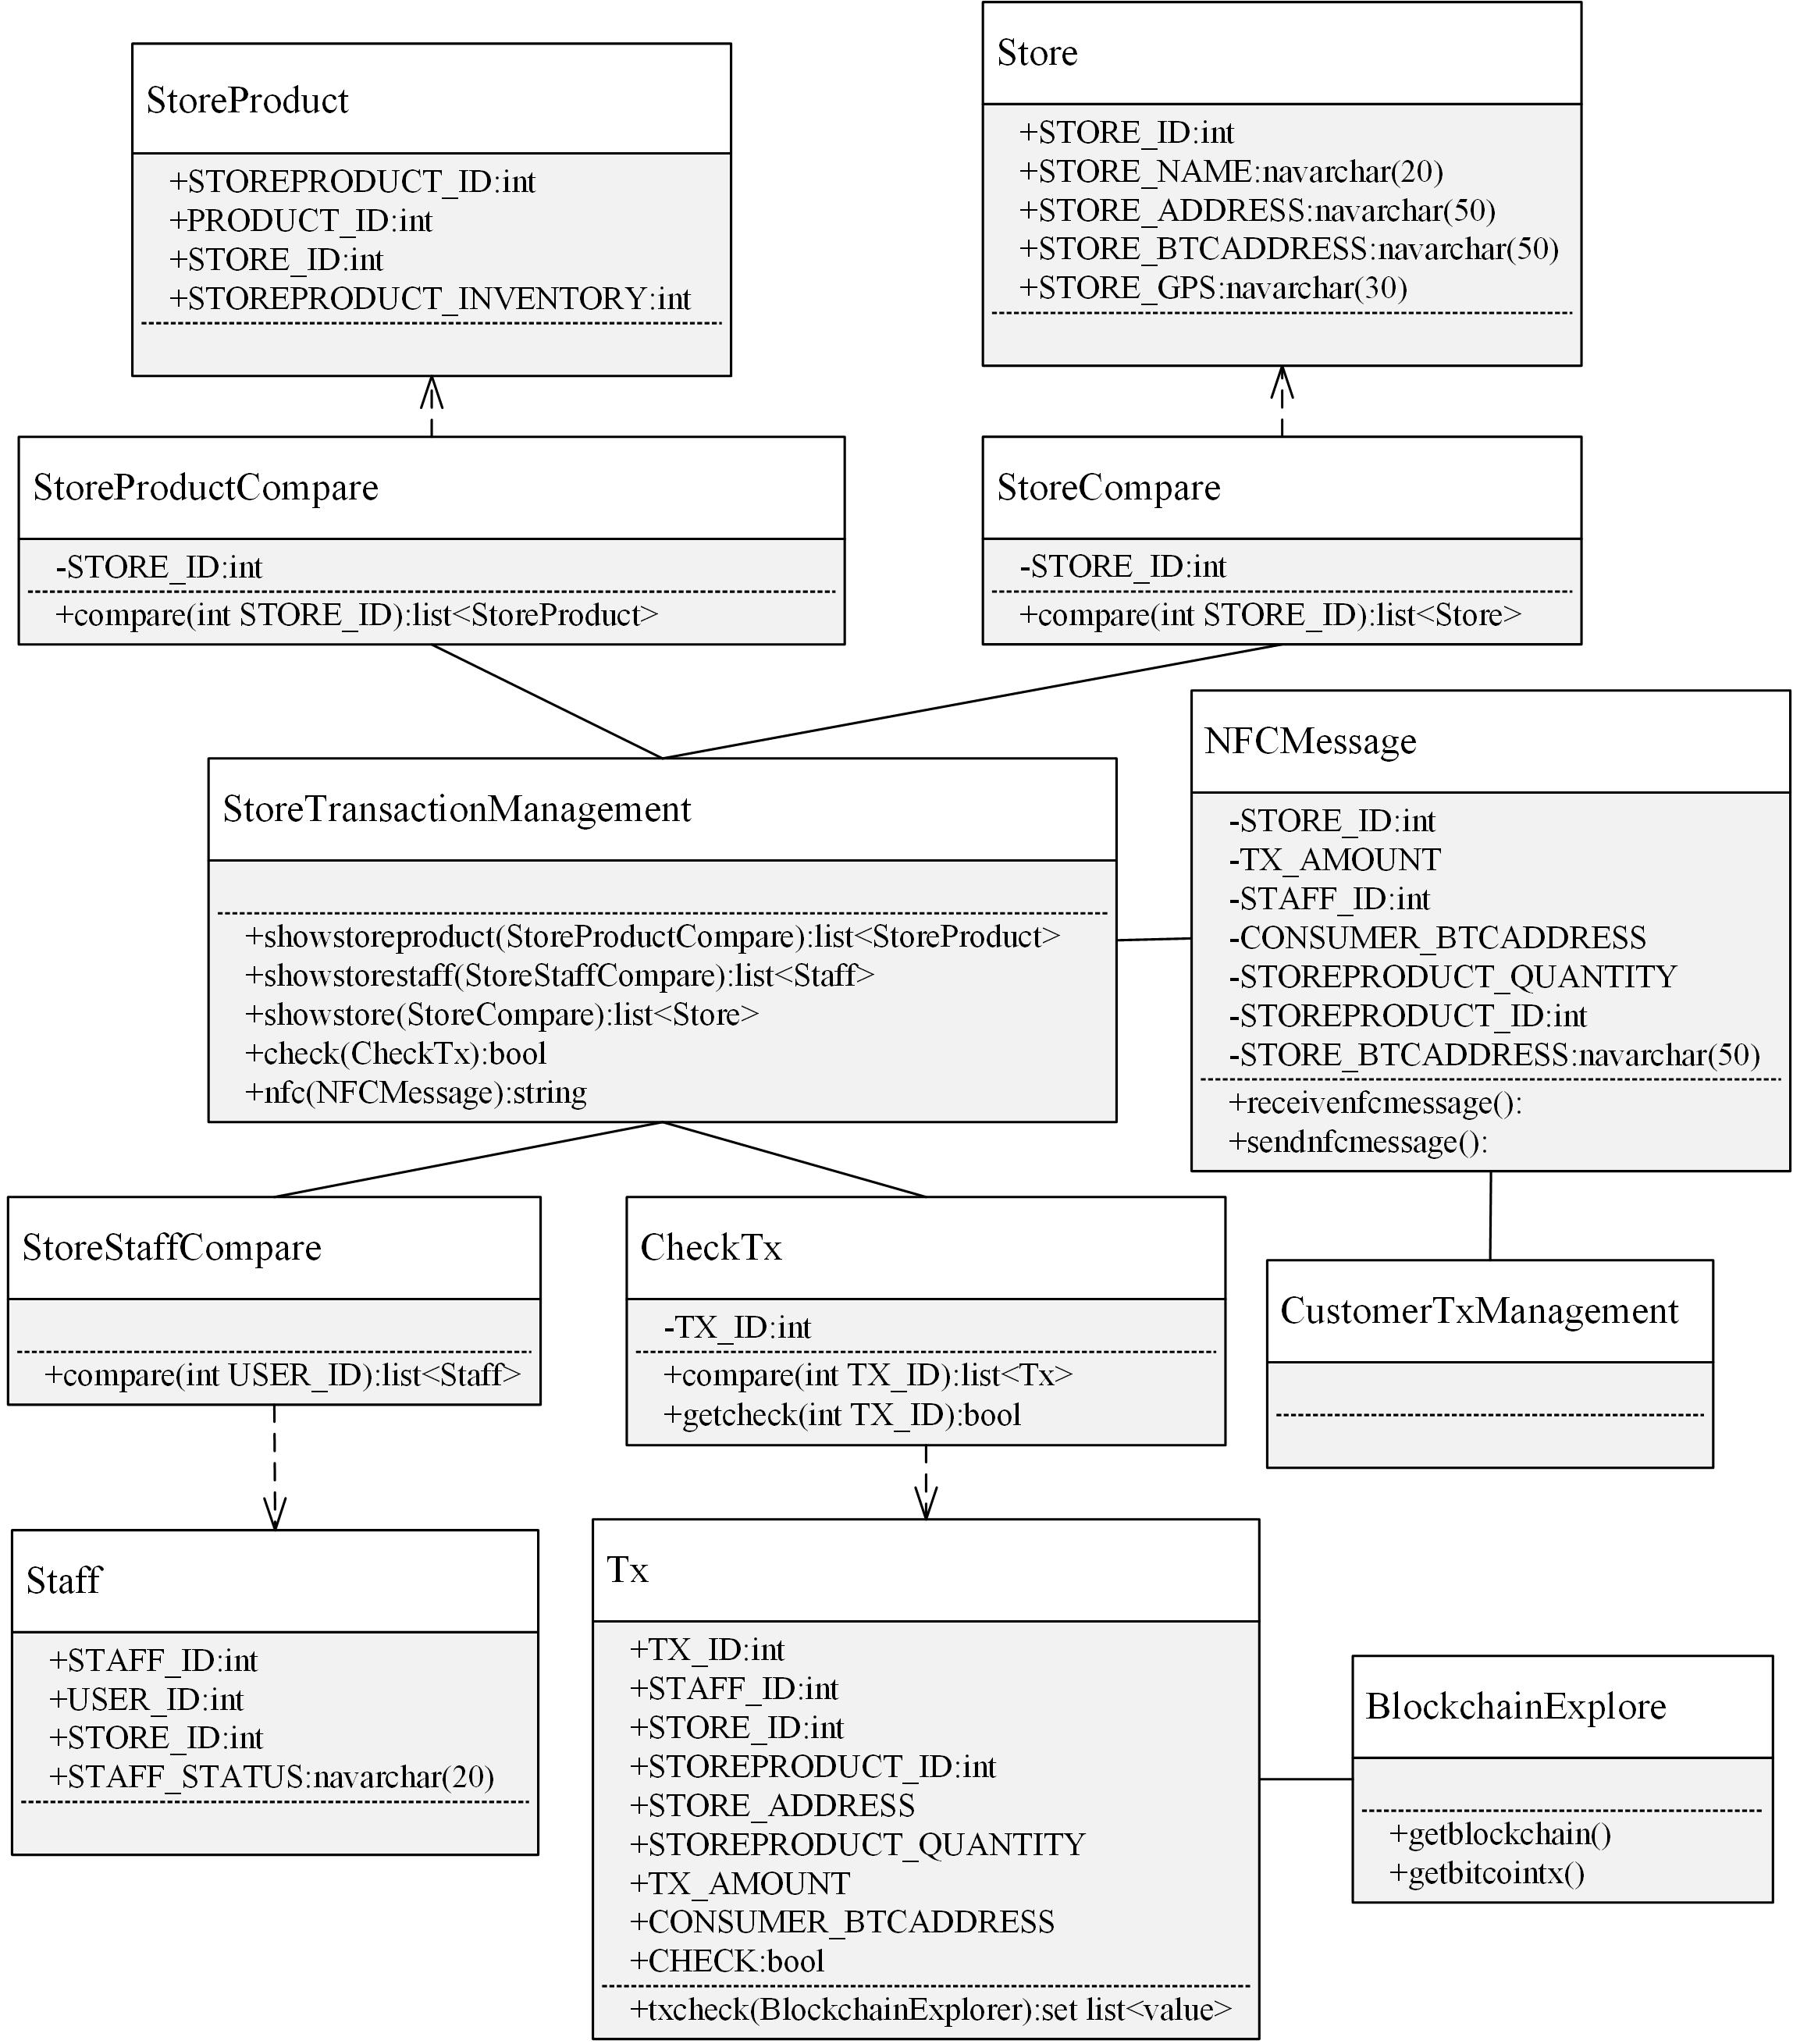
\includegraphics[width = 0.9\textwidth]{c5.jpg}
		\caption{商家交易管理模塊類圖}\label{c5}
	\end{figure}


圖\ref{time4}為商家交易管理時序圖,以下為流程說明:

	\begin{figure}[!htbp]
		\centering
		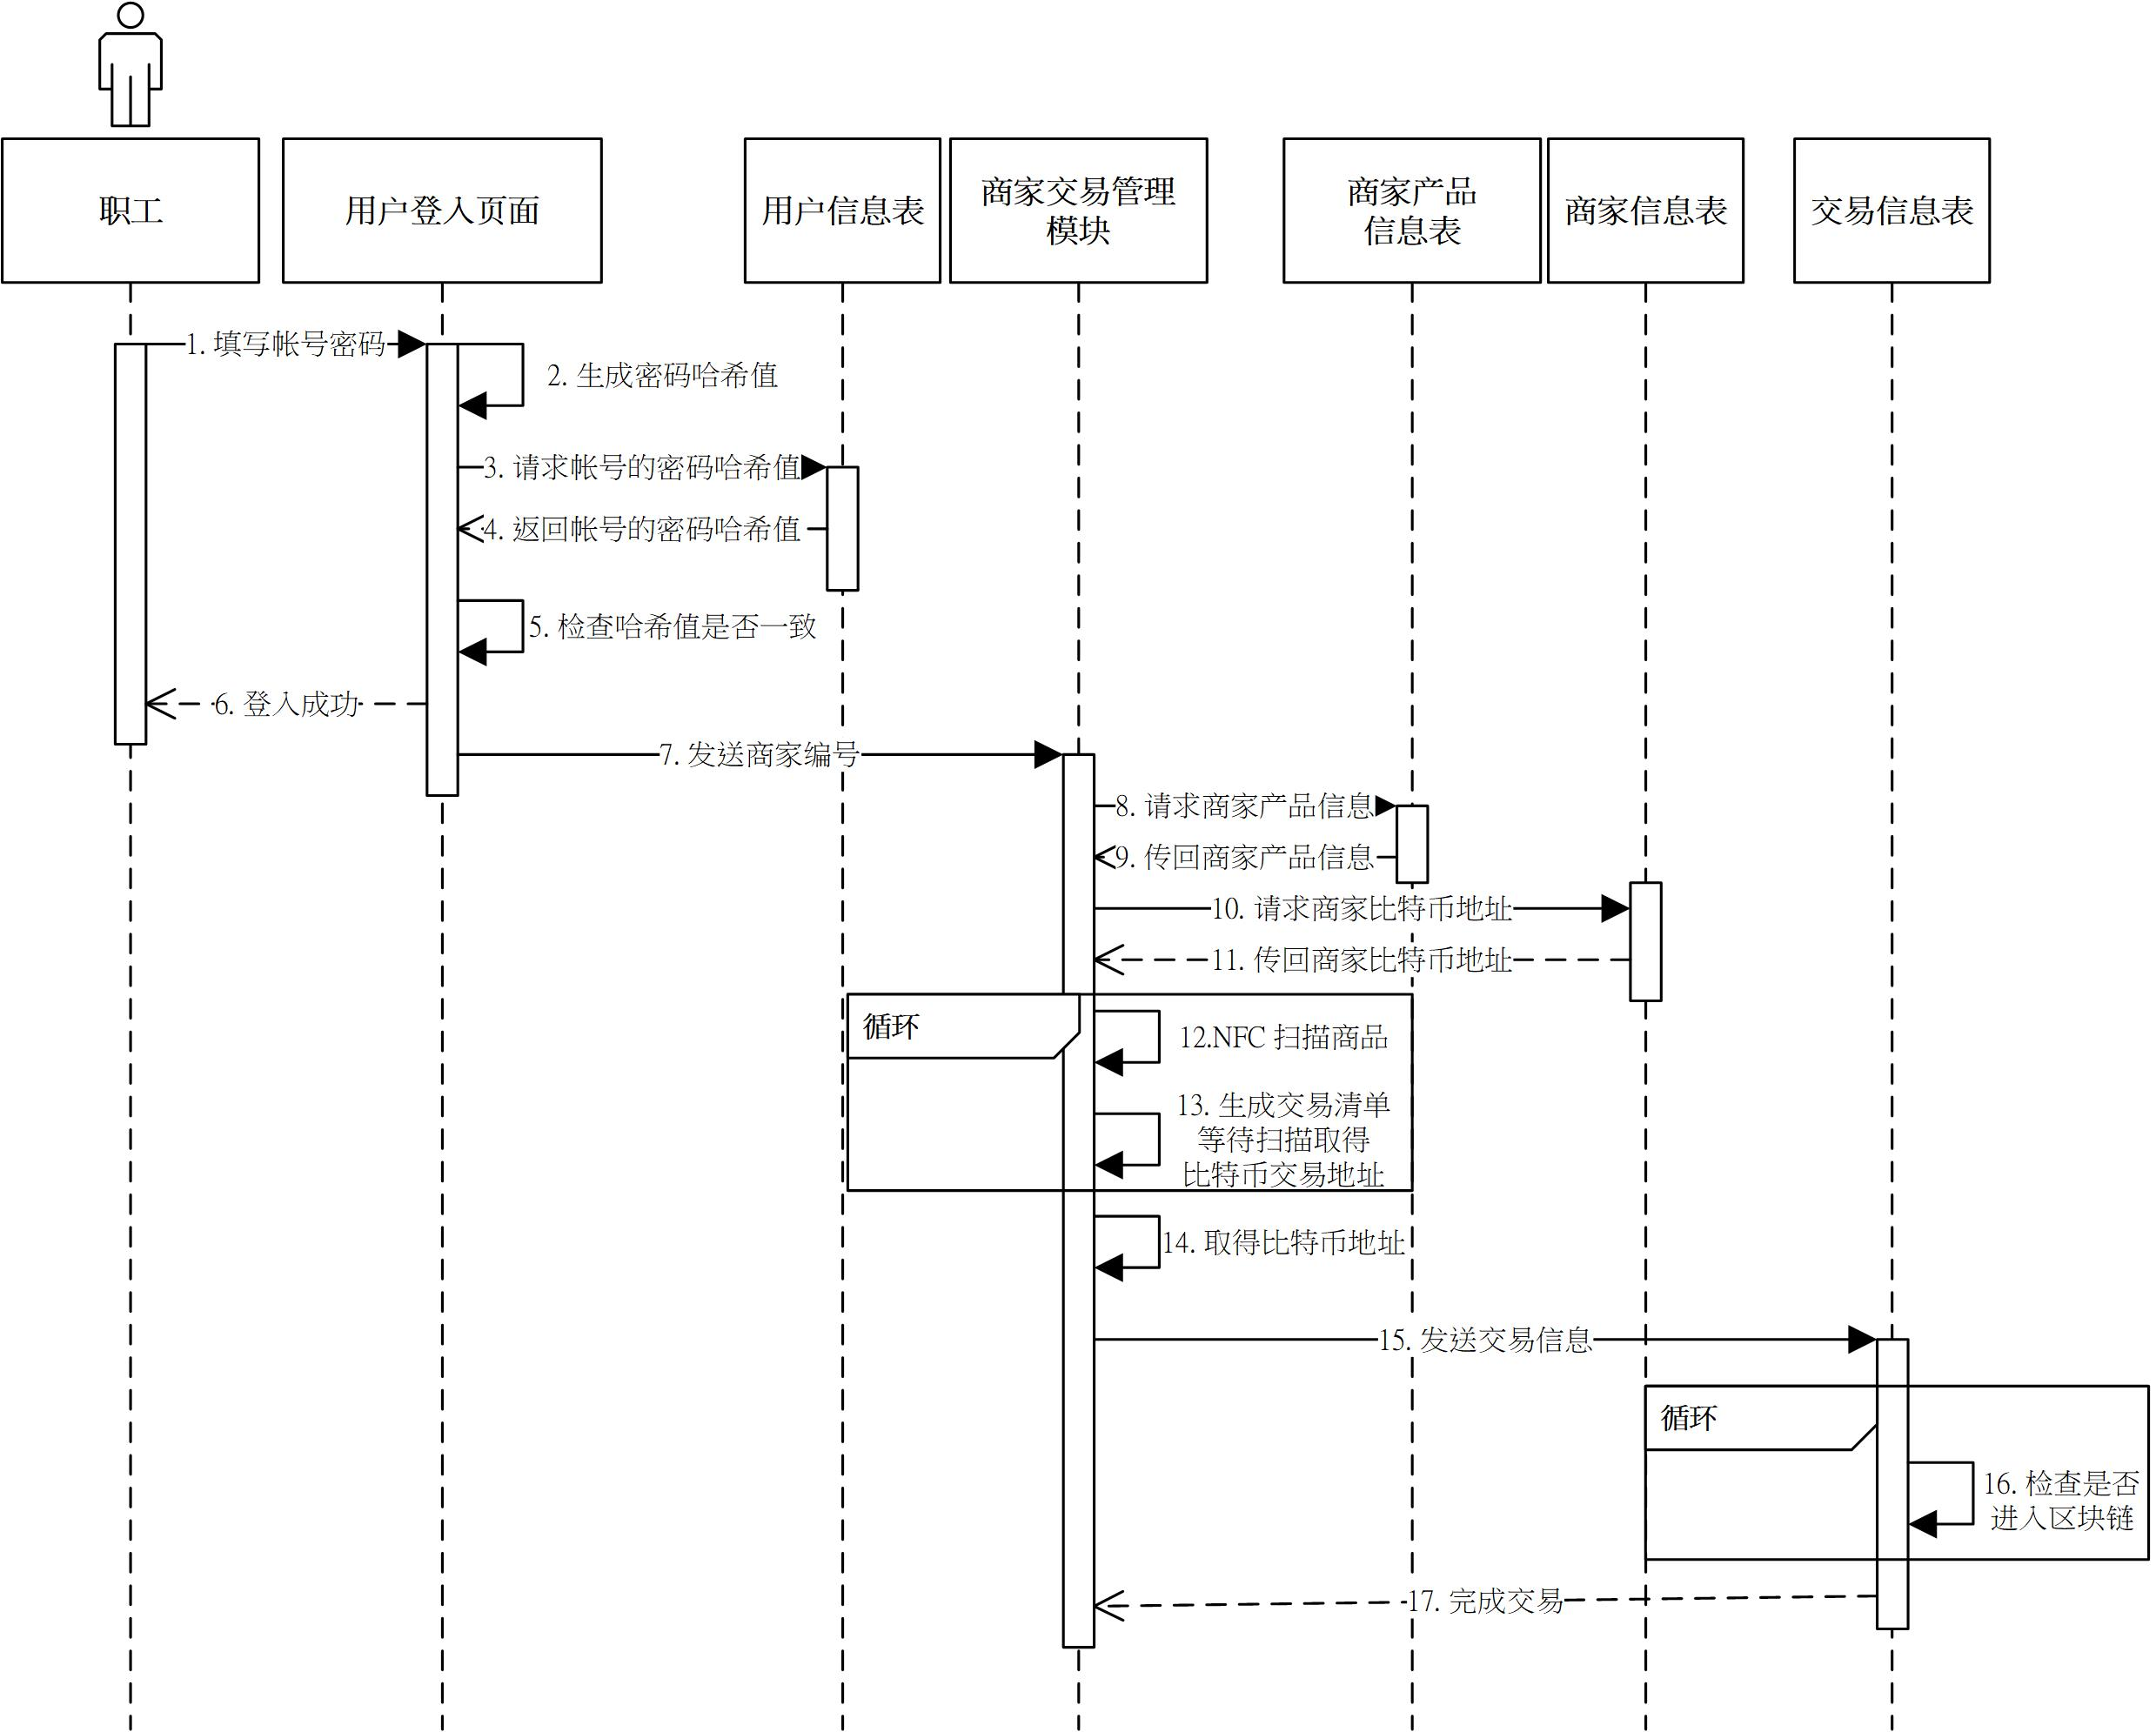
\includegraphics[width = 1\textwidth]{time4.jpg}
		\caption{商家交易管理時序圖}\label{time4}
	\end{figure}

	\begin{enumerate}
	\item 首先職工填寫用戶的帳號密碼到用戶登入頁面。
	\item 用戶登入頁面模塊將用戶填寫的密碼透過哈希算法生成本地端的用戶密碼哈希值。
	\item 將用戶填寫的帳號發送到用戶信息表請求遠端的用戶密碼哈希值以及商家編號。
	\item 用戶信息表傳回遠端的用戶密碼哈希值。
	\item 用戶登入頁面模塊進行本地用戶密碼哈希值和遠端用戶密碼哈希值比對是否一樣。
	\item 倘若一致則登入成功。
	\item 此時用戶登入頁面向商家交易管理模塊發送商家編號的信息,商家交易管理模塊將信息保存。
	\item 商家交易管理模塊向商家產品信息表請求與商家編號相關的所有商家產品信息。
	\item 商家產品信息表傳回所有與商家相關的商家產品信息至商家交易管理模塊。
	\item 商家交易管理模塊向商家信息表請求商家比特幣地址信息。
	\item 商家信息表將商家比特幣地址信息傳回到商家交易管理模塊。
	\item 商家產品信息表將所有與商家編號有關的商家產品信息傳回到商家交易管理模塊,此時商家交易管理模塊已經有完整的商家產品信息以及商家信息。將帶有RFID標籤的商品透過NFC線圈進行感測對應到相關的商家產品信息。
	\item 將產品信息建立交易清單顯示在移動裝置的屏幕上,等待顧客的手持裝置進行感應,感應的同時會將交易清單以及商家比特幣地址傳送到顧客交易管理模塊。

	\item 在感應的同時顧客交易管理模塊會將比特幣錢包模塊中的比特幣地址提交給商家交易管理模塊。
	\item 商家交易管理模塊發送信息至交易信息表查找該筆交易信息。
	\item 交易信息表不斷的向區塊鏈檢視器查找該筆比特幣交易是否已經被寫入比特幣區塊鏈內,倘若寫入區塊鏈則將交易信息的CHECK信息由"0"改為"1"。
	\item 交易信息表傳回該筆交易的CHECK已經為"1"則完成交易
	
	\end{enumerate}

	在比特幣系統中,使得一筆比特幣交易得到比特幣網路的認可,需要等待六個區塊的交易驗證,相當於需要費時60分鐘的時間等待一個交易的完成,這使得比特幣交易在商家進行小額交易造成很大的不便,因此為了在BRTMS中改善此問題,便導入了基於Green Address錢包的多重簽章算法,使得交易時間可以從60分鐘的等待時間,縮短為一秒鐘左右。圖\ref{c7}為商家Government Green Address交易管理模塊類圖,在此模塊類圖中針對Tx類中添加ggatxcheck()方法,使得商家交易管理模塊可以支持Government Green Address地址格式的辨別,當檢測到為Government Green Address地址格式,將交易信息中的CHECK欄位修改為"1",這使得比特幣交易信息可以在平均一秒鐘的時間得到交易確認,ggatxcheck()方法需要調用BlockchainExplore類中的getblockchain()取得比特幣區塊鏈的信息以及getbitcointx()方法得到比特幣交易信息。在GovernmentGreenaddressCheckTx類中提供compare()方法可以針對Government Green Address地址向Tx類查詢相關信息以及ggatxcheck()方法檢測該筆交易是否存儲於交易信息中的CHECK值已經被修改為"1"。

	

	\begin{figure}[!htbp]
		\centering
		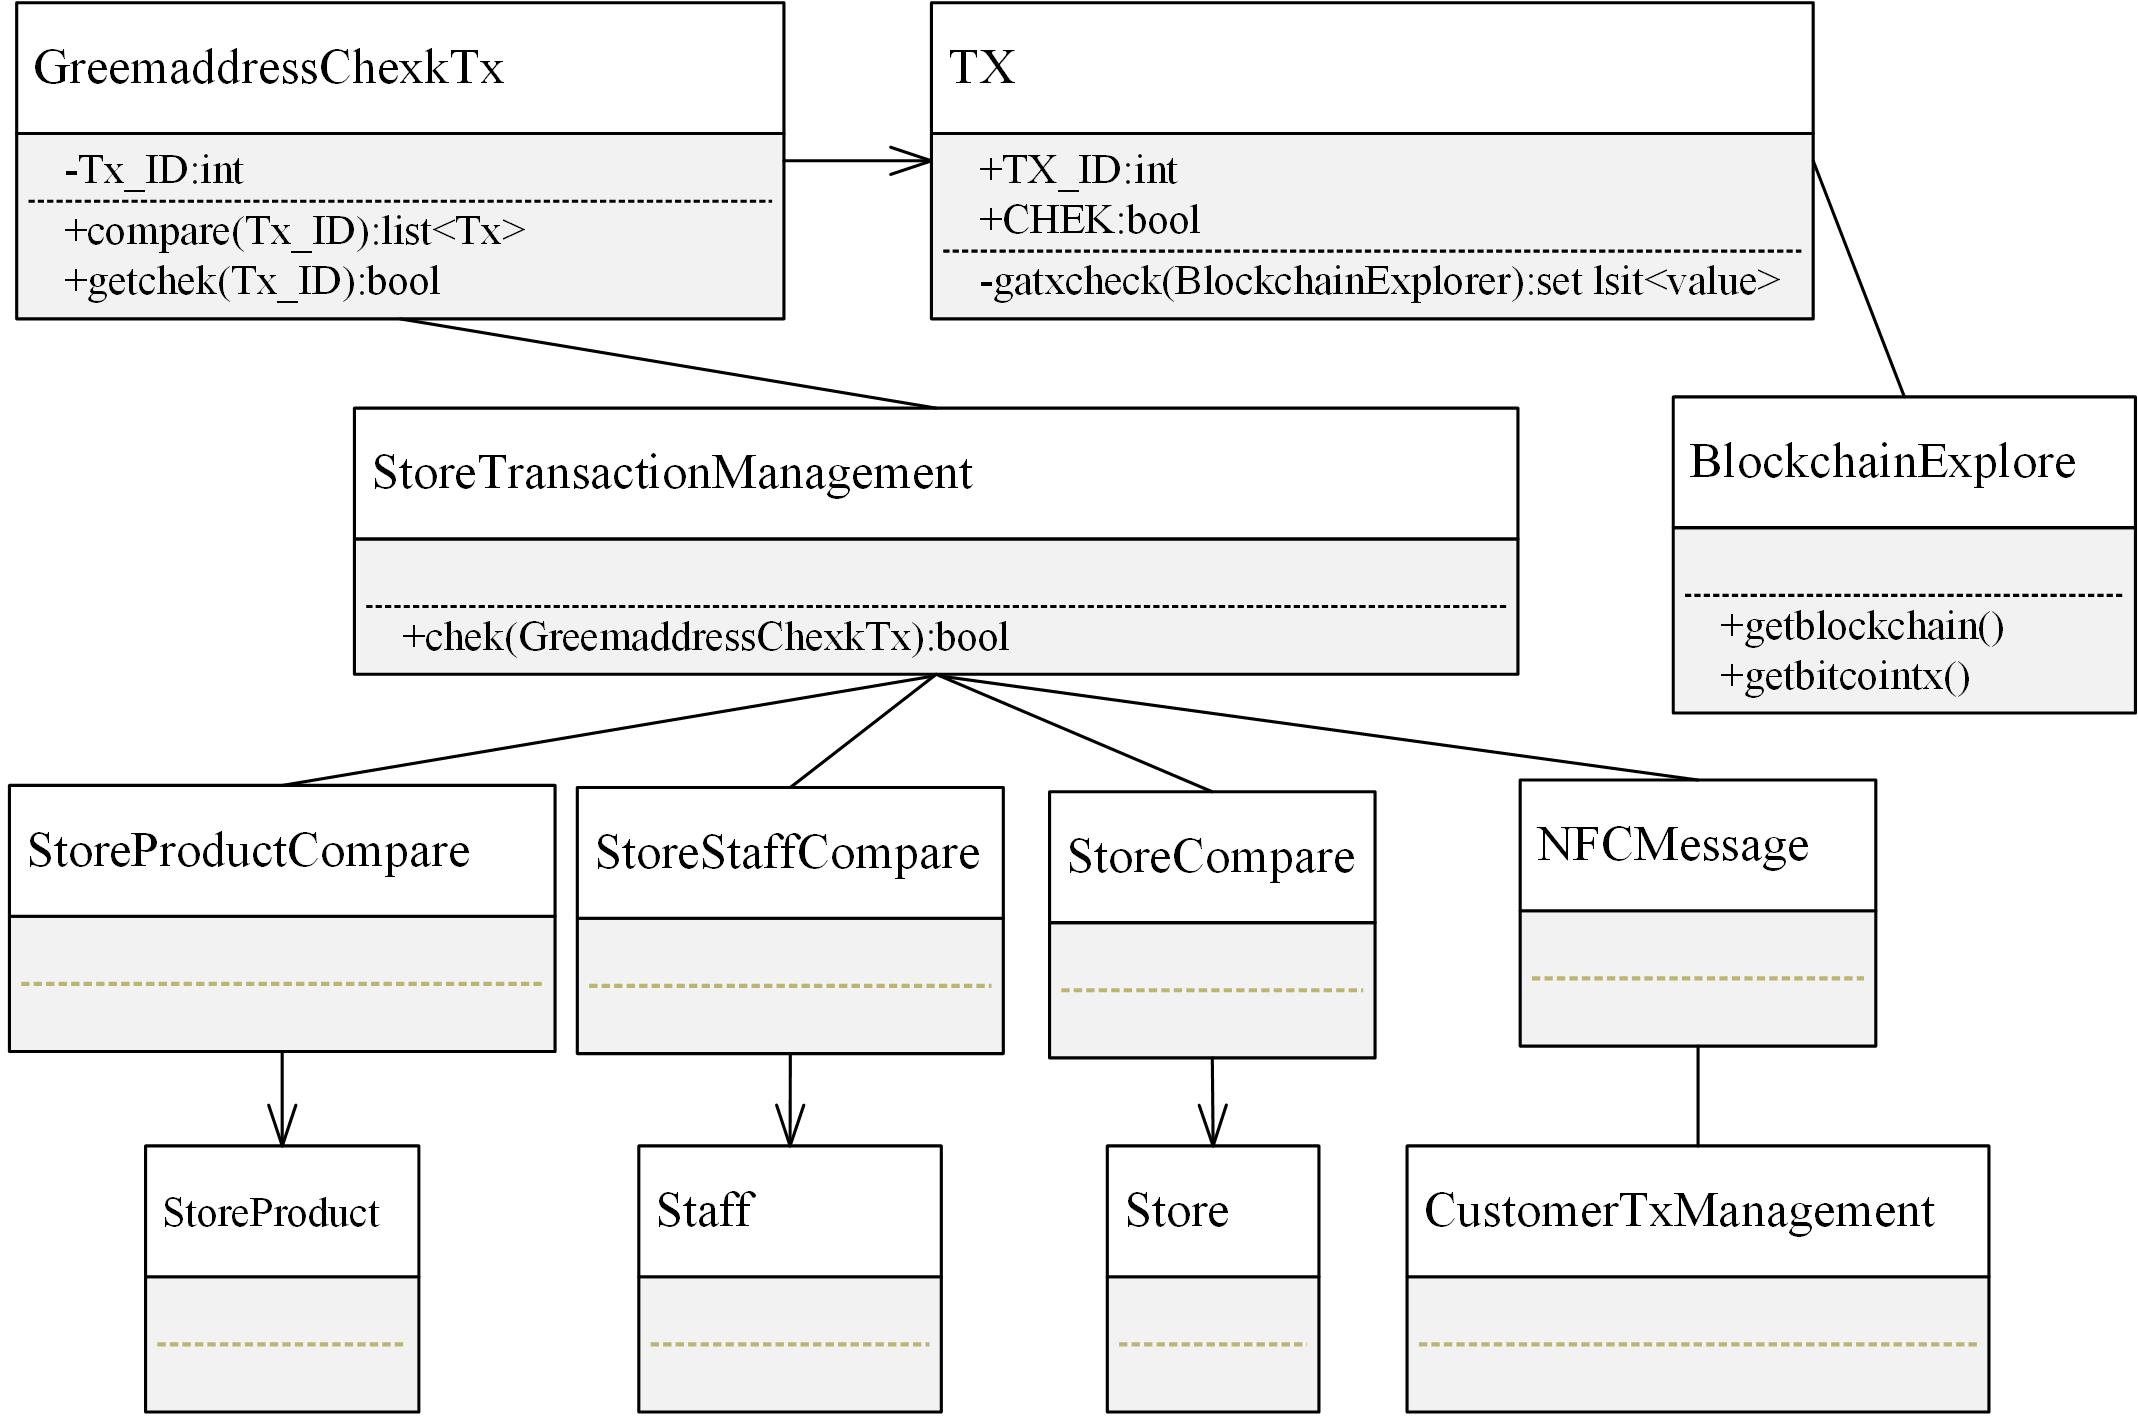
\includegraphics[width = 0.8\textwidth]{c7.jpg}
		\caption{商家Government Green Address交易管理模塊類圖}\label{c7}
	\end{figure}



\subsubsection{(五)顧客交易管理模塊}
在本系統中顧客需要在手持移動端安裝手機程序包括顧客交易管理模塊,使得顧客移動裝置可以支持比特幣支付、查詢過去的交易信息、以NFC通信協議接收商家交易管理模塊創建的交易信息以及詳細的商家商品信息。圖\ref{c4}為顧客交易管理模塊類圖,在CustomerTxManagement 類中包括六個⽅法,分別為顯⽰所有該⽤⼾擁有⽐特幣交易信息相關的交易明細的showtx() ⽅法、取得交易信息後取得相對應的商家產品信息的showstoreproduct() ⽅法、檢查於交易信息表中的交易信息CHECK 欄位的值是否已經被填⼊"1" 的check() ⽅法、發送詳細的交易信息⾄交易信息表保存的sendtx2table()⽅法、透過NFC 協議接收於StoreTransactionManagement 類所創建的交易信息以及發送⽤⼾⽐特幣地址的nfc() ⽅法,最後是控制⽐特幣錢包的bitcoinpayment() ⽅法。CheckTx類中的getcheck() ⽅法可以向Tx 類詢問該筆交易是否已經得到認證,TxCompare 類中的compare() ⽅法提供⽤⼾向交易信息表查找與⽤⼾交易信息相關的交易,TransferTx類中的sendtx() ⽅法是將顧客完成交易的交易信息提交到交易信息表,BitcoinPay 類使⽤pay() ⽅法⽀付⽐特幣,NFCMessage 類中的receivenfcmessage() 和sendnfcmessage()分別為透過NFC 協議發送以及接收交易信息和顧客⽐特幣地址。StoreProductCompare類則是向StoreProduct 類請求顧客移動裝置中所有交易信息中相關的商家商品。

	\begin{figure}[!htbp]
		\centering
		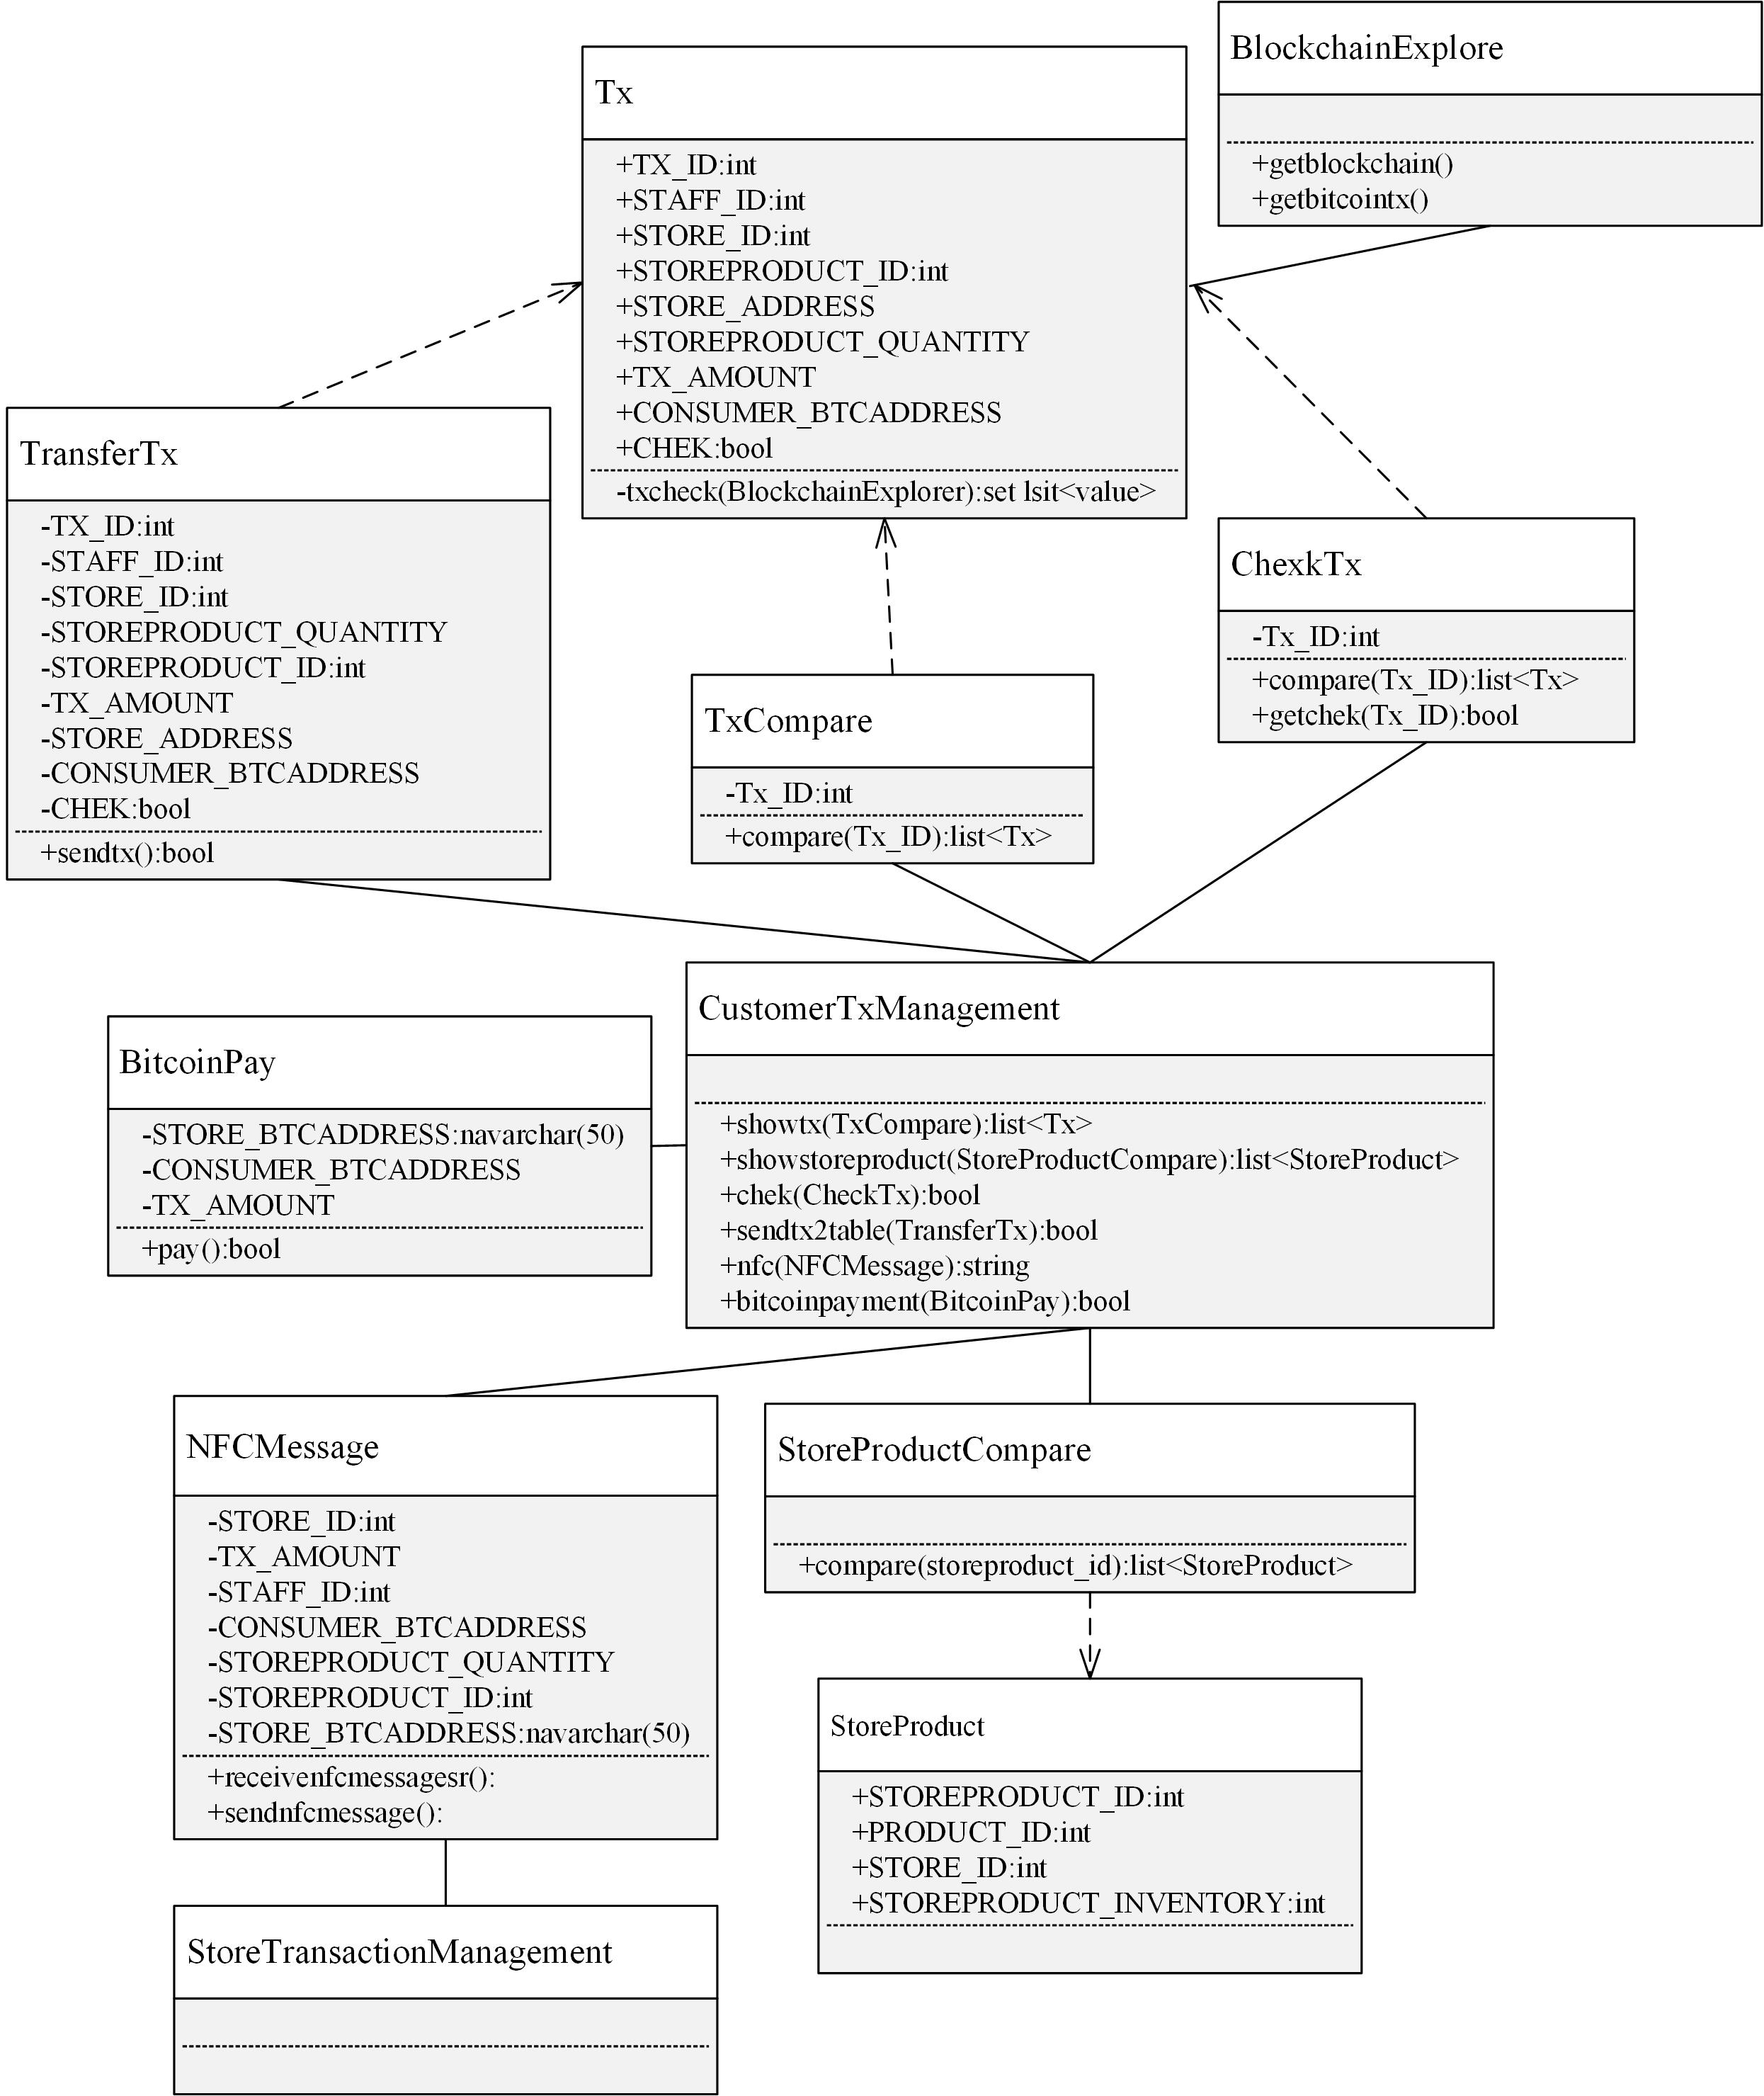
\includegraphics[width = 0.9\textwidth]{c4.jpg}
		\caption{顧客交易管理模塊類圖}\label{c4}
	\end{figure}

	

	圖\ref{time5}為顧客交易管理時序圖,以下為流程說明:

	\begin{figure}[!htbp]
		\centering
		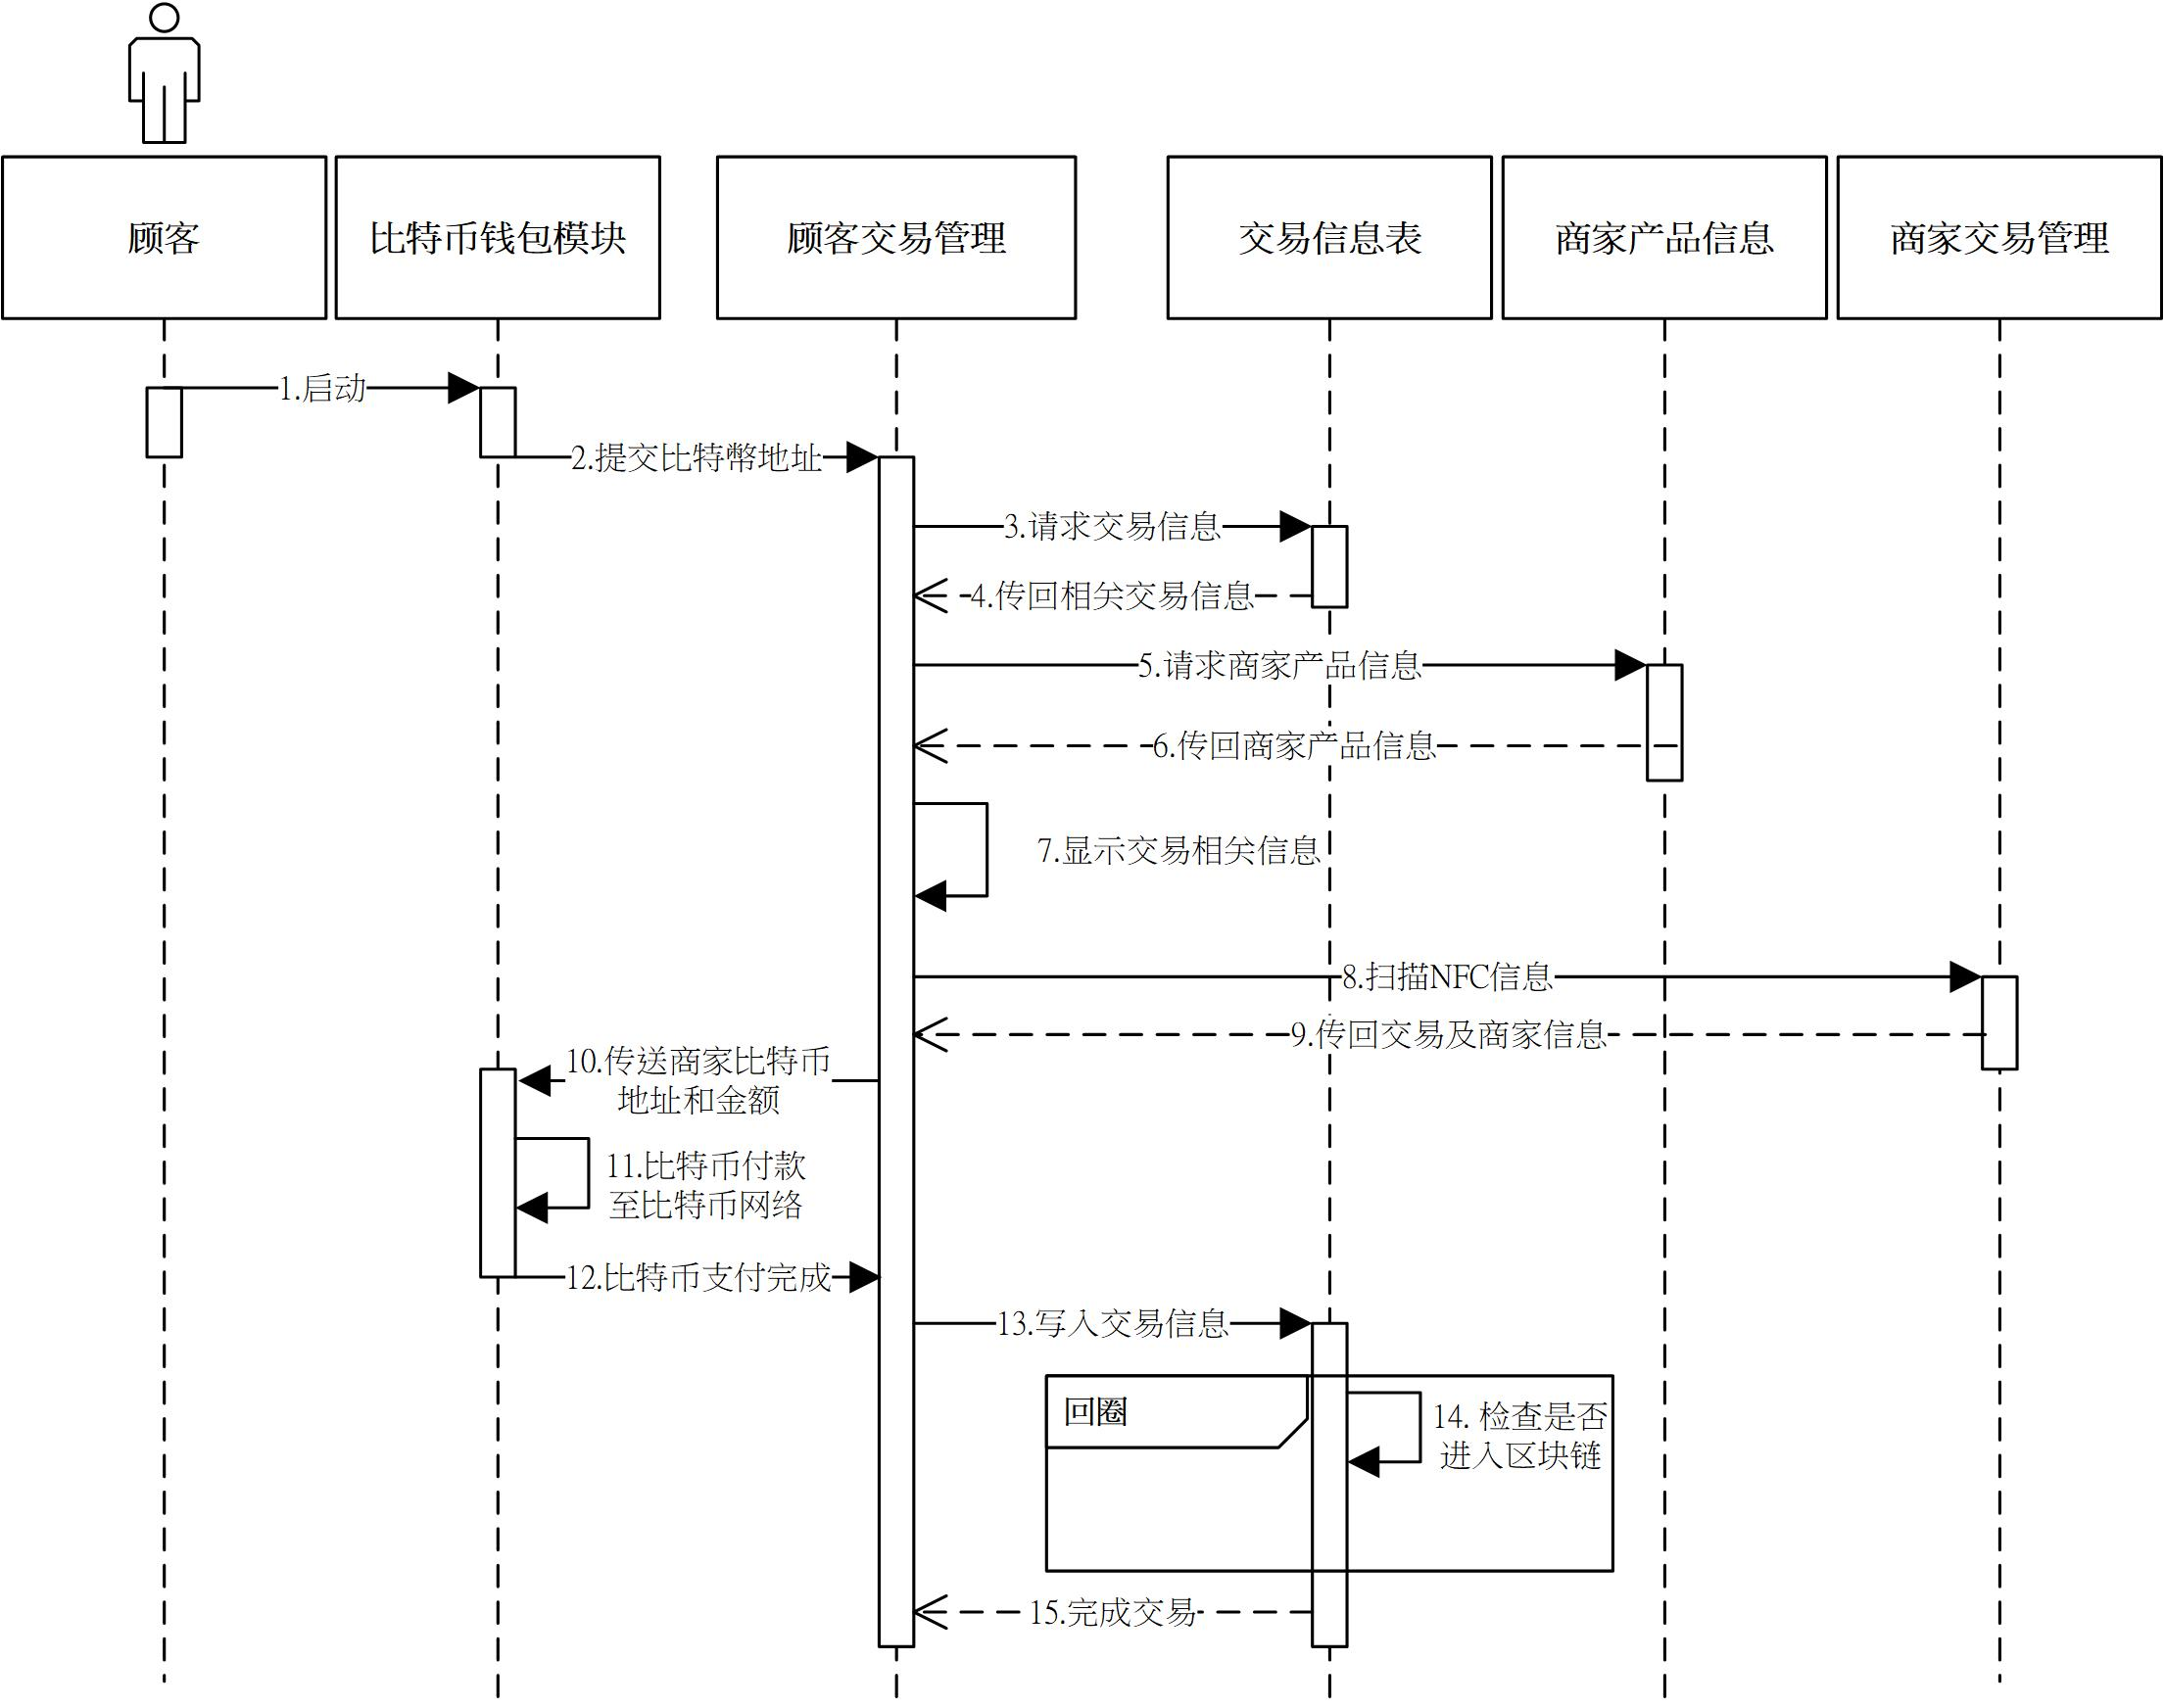
\includegraphics[width = 1\textwidth]{time5.jpg}
		\caption{顧客交易管理時序圖}\label{time5}
	\end{figure}

	\begin{enumerate}
		\item 顧客啟動比特幣錢包管理模塊,屆時比特幣錢包管理模塊再同步最新的區塊鏈信息至手機本地端,並將與手機本身存在的比特幣地址進行核對。
		\item 將所有在比特幣錢包模塊的地址提交到顧客交易管理模塊。
		\item 顧客交易管理模塊將所有拿到的比特幣地址發送到交易信息表,請求完整的交易信息內容。
		\item 交易信息表將概要的交易信息傳回顧客交易管理,此時的交易信息並非相當完整,只有商家產品編號。
		\item 為了使得交易信息更加的完整可以顯示更多的商家產品說明,便將手機本地端數據庫存在的商家產品編號向商家產品信息表提出請求更詳細的說明。
		\item 商家產品信息表傳回詳細的商家產品信息到顧客交易管理模塊。
		\item 顧客交易管理模塊將收到的信息顯示在畫面上。
		\item 當顧客前往商家時,商家掃描完所有顧客欲購買的商家比特幣地址、商家商品、數量、價格以及應付金額之後,便向商家交易管理啟動NFC準備等待顧客的手持裝置進行信息傳輸,此時的顧客將手持裝置與商家手持裝置靠近。
		\item 商家管理模塊透過NFC將交易清單信息傳送到顧客交易管理模塊。
		\item 在商家交易管理模塊重送的交易清單信息當中,包括商家的比特幣地址信息與應付金額,此時顧客交易管理模塊將比特幣地址信息傳送到比特幣錢包模塊。
		\item 在比特幣錢包模塊當中使用secp256k1算法簽署比特幣交易信息,並將交易信息廣播到比特幣網路當中,此時該筆交易信息會進到⽐特幣網絡中的交易緩存等待礦工解出工作量證明的問題,將該筆交易信息存儲到比特幣區塊鏈。
		\item 在完成比特幣簽名後,會生成比特幣的交易哈希值,比特幣錢包管理模塊將比特幣交易哈希值傳送到顧客交易管理模塊。
		\item 顧客交易管理模塊請求交易信息表將比特幣交易哈希值寫入。
		\item 完成寫入後,交易信息表模塊會調用比特幣區塊鏈檢視器的相關函數,不斷檢查該筆比特幣交易是否已經從未確認交易轉變成已確認交易。倘若發現已經確認,則將交易信息表中CHECK欄位的信息從"0"修改為"1"。
		\item 發現交易信息中的CHECK值為"1"之後,便發送完成交易的信息到顧客交易管理模塊。
	\end{enumerate}

	圖\ref{c6}為BRTMS中的顧客Government Green Address交易管理模塊類圖,以下將說明採用Government Green Address與未採用Government Green Address技術的顧客交易管理類圖設計之間的差異。於Tx類中添加ggatxcheck()方法,該方法可以不斷檢查交易信息表中的交易是否來自Government Green Address地址,倘若是則不需要等待區塊鏈的驗證時間可以即刻認定該筆交易為有效,快速提交比特幣交易速度。GovernmentGreenaddressCheck類中compare()方法是為了查找與TX\_ID相符的交易信息,getchek()方法則是向交易信息表中詢問符合TX\_ID的交易信息是否已經被修改為"1"。其中GovernmentGreenaddressBitcoinPay類中的multiplesignature()方法可以實現多重簽章算法,使得本系統可以支持即時交易。governmentgreedaddresspay()方法是將多重簽章算法廣播報導比特幣網路。


	\begin{figure}[!htbp]
		\centering
		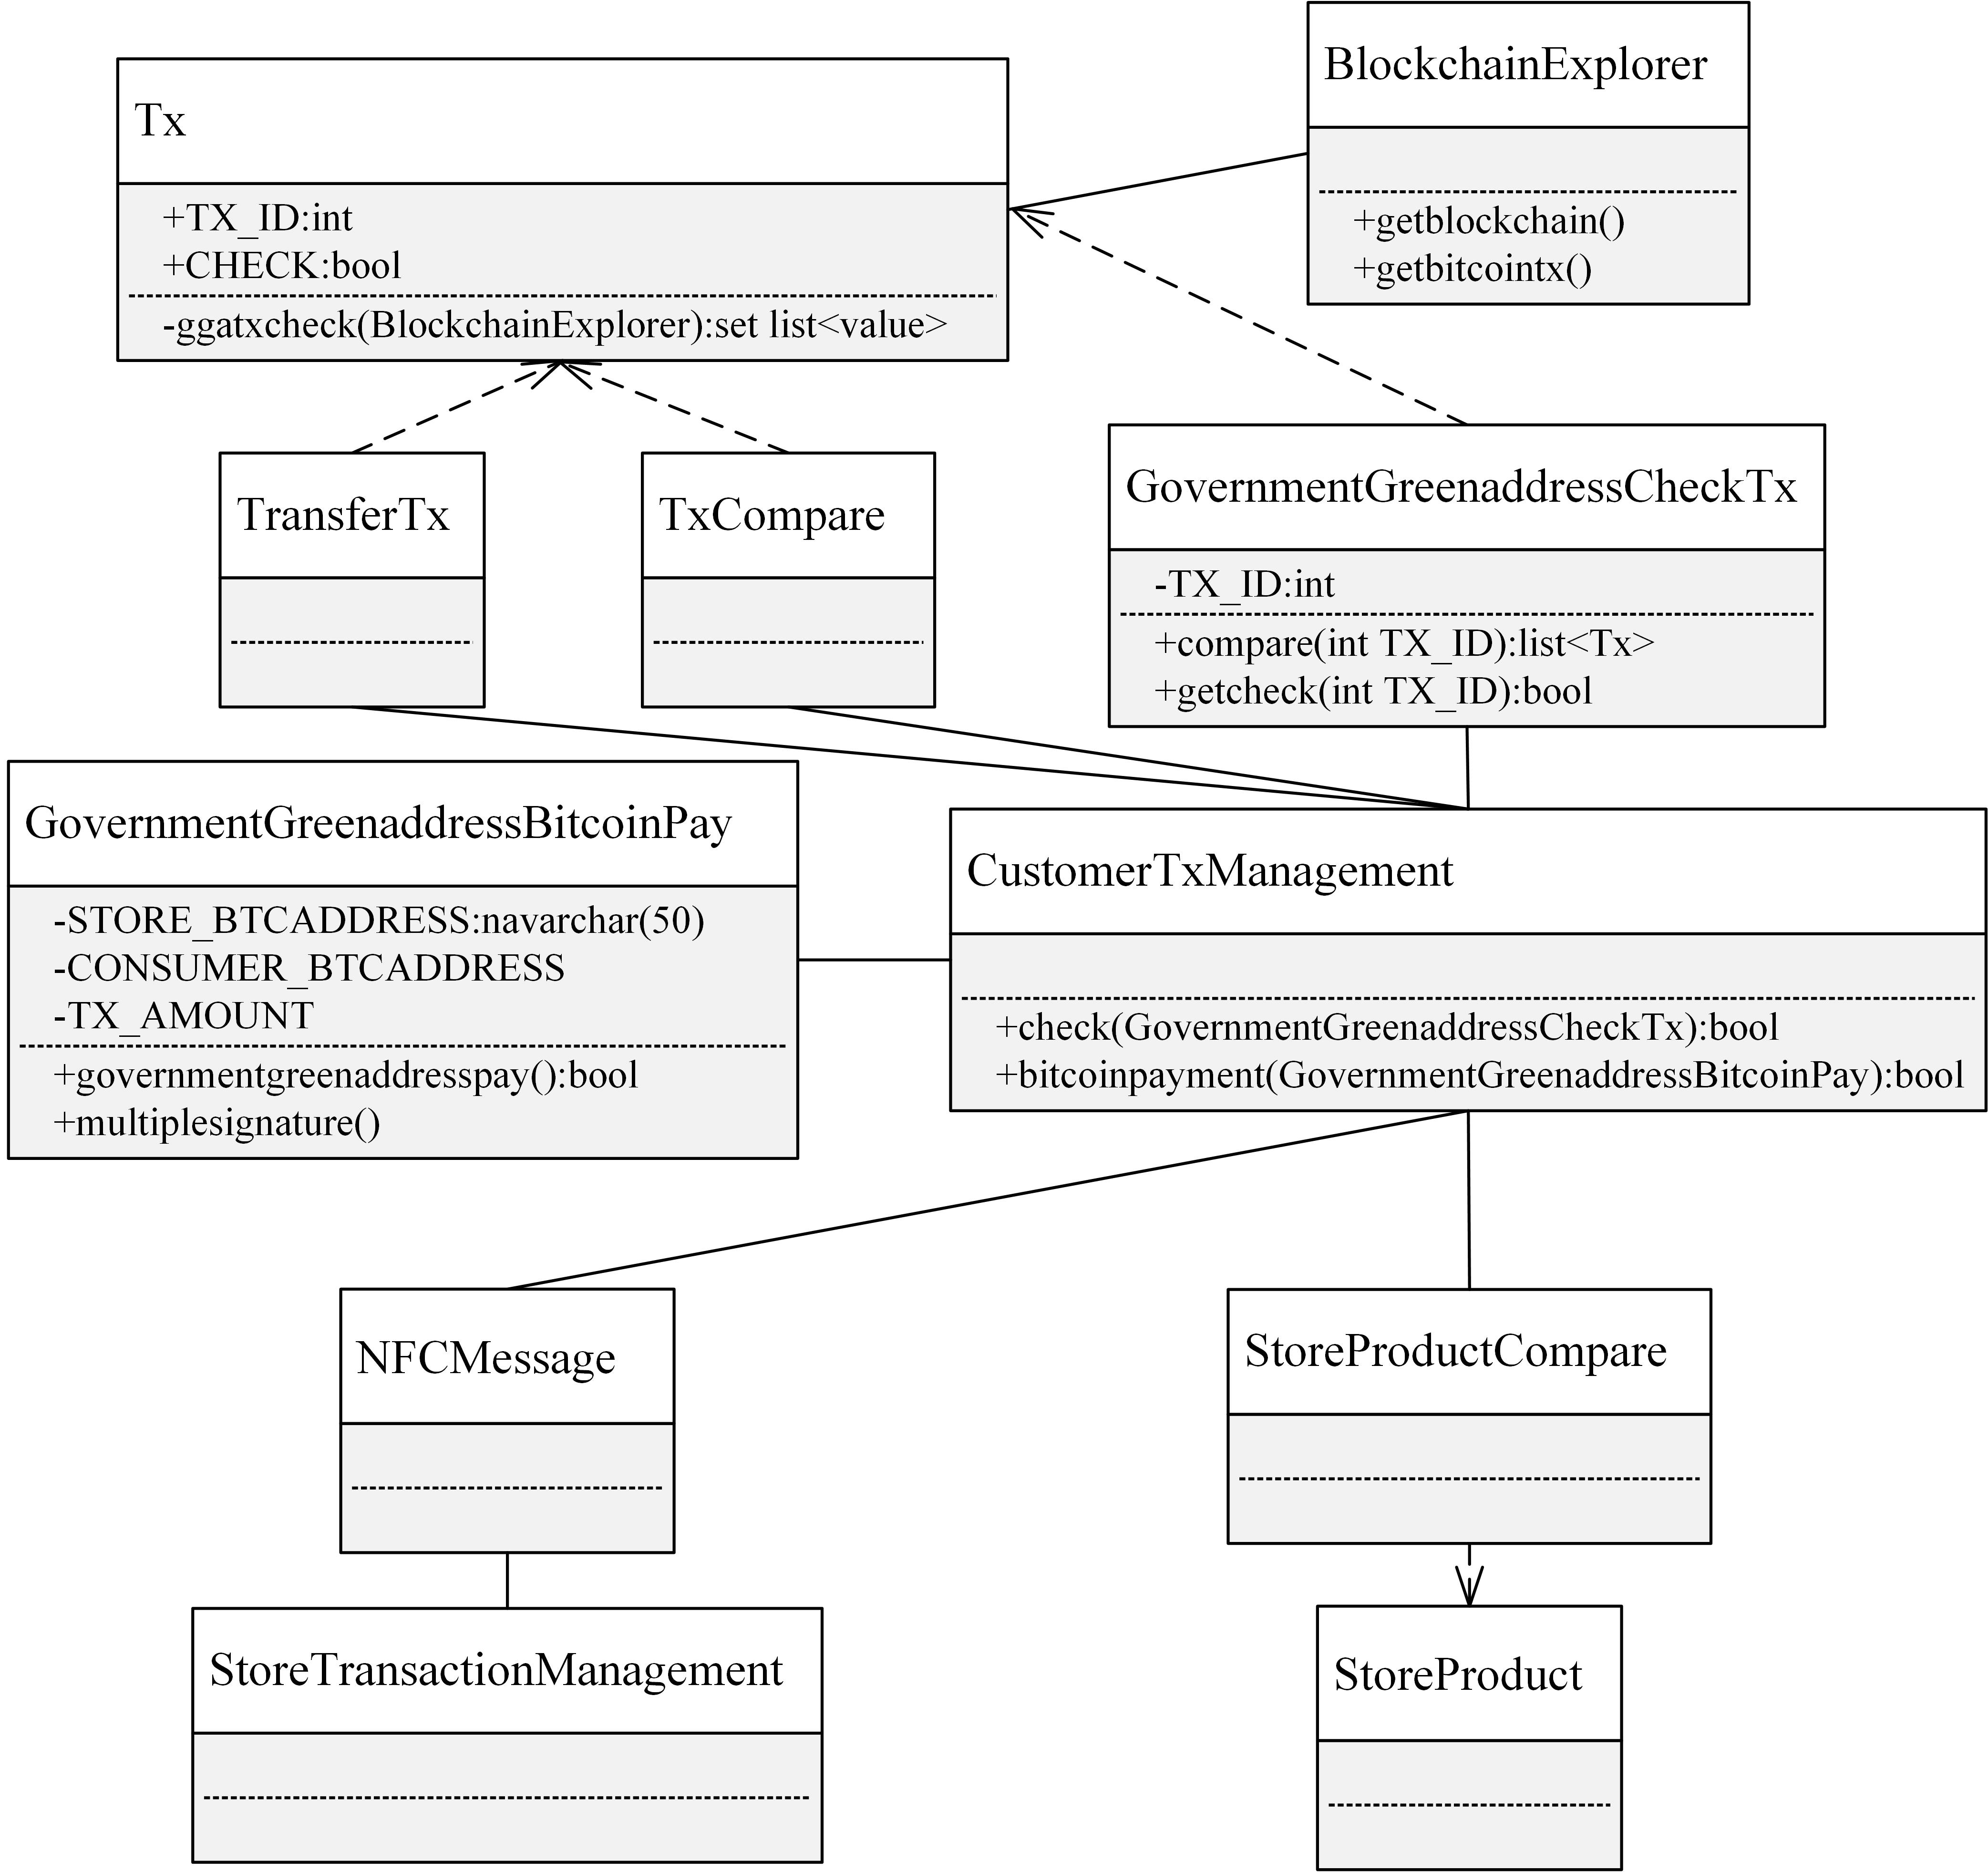
\includegraphics[width = 0.7\textwidth]{c6.jpg}
		\caption{顧客Government Green Address交易管理模塊類圖}\label{c6}
	\end{figure}

\section{系統實現}

% \section{區塊鏈的實名交易監督系統實現}

為了驗證和證明所提議的BTMS用於比特幣支付收款監督的可行性和有效性,將其運行在用於商家商品管理和維護的Java應用程序的SMIMSS子系統,用於商家職工的運行在Android App上的SMCTSS以及運行在App上的用於顧客的CMPTSS。
如圖\ref{fig5}所示,SMIMSS 的 Java應用程序可以幫助商家登錄到系統或創建一個新帳戶。 授權商家成功登錄系統後,商家可以插入或更新產品列表,如圖\ref{fig6}所示。實現的SMIMSS Java應用程序執行前面部分中所述的功能。

\begin{figure}[!htbp]
	\centering
	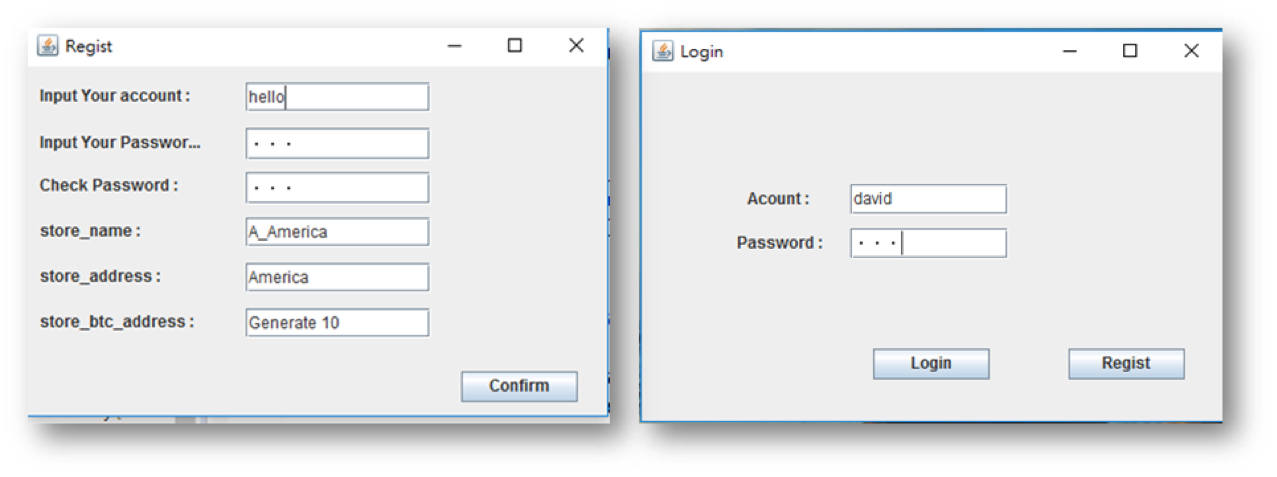
\includegraphics[width = 0.9\textwidth]{fig5.png}
	\caption{SMIMSS的Java應用程序的註冊和登錄界面}\label{fig5}
\end{figure}

\begin{figure}[!htbp]
	\centering
	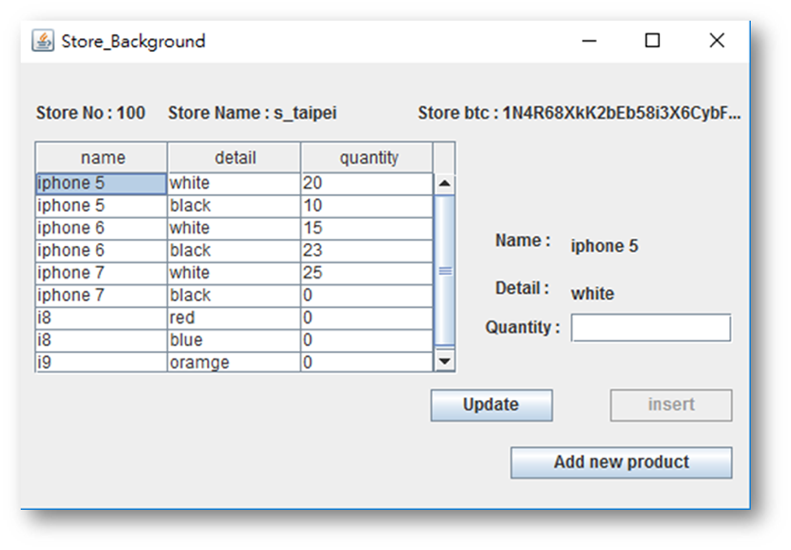
\includegraphics[width = 0.6\textwidth]{fig6.png}
	\caption{在SMIMSS中插入或更新授權商家的產品目錄}\label{fig6}
\end{figure}

商家的產品信息可以通過RFID標籤掃描,存儲到雲端數據庫中,商家職工可以使用實現的SMCTSS Android客戶端,啟用NFC監聽器,從購物車中的顧客購買產品中讀取RFID標籤信息。 在如圖\ref{fig7}所示的第一項活動中,商家職工必須登錄才能獲得授權訪問SMCTSS功能。 然後,在第二項活動中,SMCTSS應用程序可以通過使用SMIMSS中應用的雲數據庫檢查產品RFID標籤信息並將其展示給顧客,從而將掃描的產品列入購物車。 在圖\ref{fig7}的第三項活動中,顧客可以要求職工刪除購買物品以,並確認最終交易清單。 最後,SMCTSS應用程序將自動使用比特幣測試網絡(Bitcoin Testnet)\supercite{bitcointestnet}幫助職工確認發布此比特幣交易的收款人地址,如圖\ref{fig7}所示。    

\begin{figure}[!htbp]
	\centering
	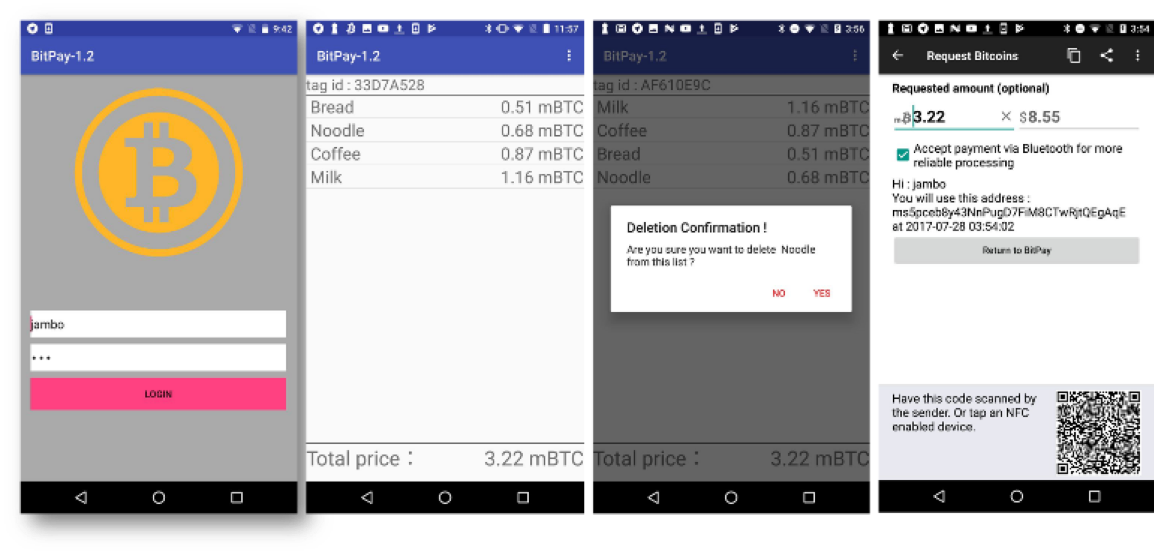
\includegraphics[width = 1\textwidth]{fig7.png}
	\caption{登錄、等待結帳的商品、刪除商品及支付確認}\label{fig7}
\end{figure}

同時,顧客將使用與SMCTSS App相對應的CMPTSS Android App通過比特幣完成採購產品交易。 如圖\ref{fig8}所示,第一個活動表示顧客確認購買產品創建交易數據庫的交易清單,第二個活動顯示包括金額和付款人比特幣地址在內的付款確認,第三個活動顯⽰該錢包交易的歷史記錄,凡是出入該錢包的所有交易都會被顯示出來,
錢包可以同時作為買⽅和賣⽅,最後在第四項活動中顯示了該筆交易詳細採購產品的交易憑據。    

\begin{figure}[!htbp]
	\centering
	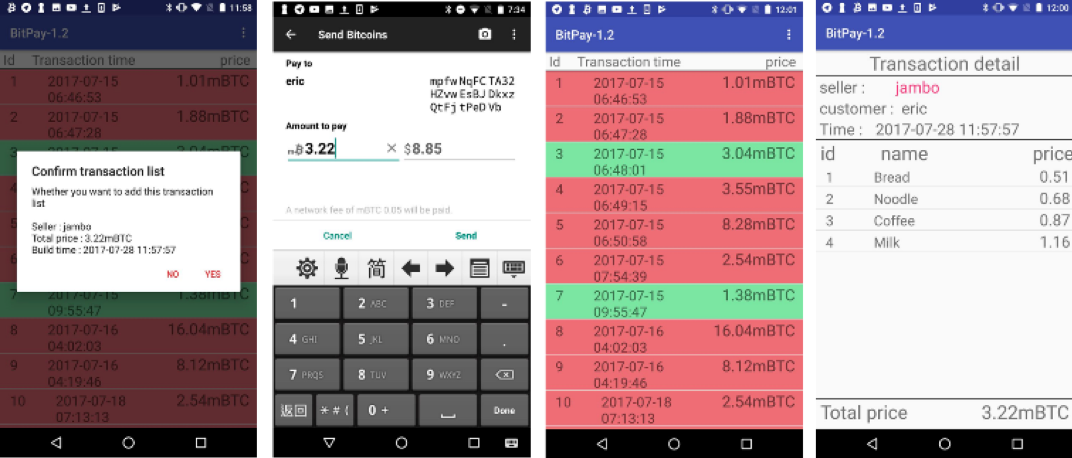
\includegraphics[width = 1\textwidth]{fig8.png}
	\caption{在CMPTSS App中,交易確認,付款確認、交易歷史記錄和發票}\label{fig8}
\end{figure}
	% Copyright (c) 2014,2016 Casper Ti. Vecto
\chapter{系统测试}
本章节内容将依据系统需求规格书与系统设计,描述关于集成测试的相关计划与内容。于本章将进⾏功能测试与性能测试,运⾏功能测试以确认本⽂所提出之系统的所有功能是否皆顺利运⾏,透过性能测试可知本系统的交易速度在优化前与优化后之间的差异,在本章中以⼿机作为⼿持移动装置的测试环境,并希望透过此章节之描述与实践,达到顺利进⾏测试⼯作之⽬的。
	\section{功能测试}
	 	本段主要是描述⽐特币的交易监督系统的测试计划。确认在系统集成前,必须先确认所有的设计组件均可正确的输出,並着重于集成系统测试(Integration Test)及验收测试(Acceptance Test)。測試過程詳如下所述:
	 		\begin{enumerate}
	 			
	 			\item 接受标准:本测试计划需要满足下列的测试接受准则: 

	 			\begin{enumerate}
					\item 本系统需要对所有列为必要(Critical、Important、Desirable)之需求作完整测试。
					\item 测试程序需要依照本测试计划所订定的程序进行,所有测试结果需要能符合预期测试结果方能接受。
					\item 以测试案例为单位,当测试未通过时,需要进行该单元的测试,其接受的准则与前一项规定相同。 
				\end{enumerate}

				\item 测试环境说明包括所采用的硬件与软件规格,分别如下:
				\begin{enumerate}
					\item 硬件规格分为系统主机以及周边设备:
					
					\begin{enumerate}
						\item 系统主机:一台以上主机,每台主机CPU为Intel Pentium 4 1.0 GHz或以上,256 MB RAM或以上,60 GB以上硬盘空间。
						\item 周边设备:⼀台以上⼿持移动装置,与⽤来代表虚拟商品的数个RFID标签,及可供测试NFC ⽤的⼿持移动装置。本測試以一台⼩⽶3 WCDMA 版及一台Google Nexus 5X分別進行測試,详细规格如表\ref{mi}、表\ref{5x}所示。
					
					\end{enumerate}
					\item 软件规格:以Windows 10 、Android 6.0.1/7.1.1操作系统為测试环境。

				\end{enumerate}
				\item 测试地点:在铭传大学桃园校区资工系实验室,透过Android手机进行的交易仿真实验,测试流程如图\ref{fig4}的示意。

%			\end{enumerate}
	 	

	 				\begin{table}[!htbp]
					\centering
					\caption{小米3手机规格表}
					\label{mi}
					\begin{tabular}{|l|l|}
					\hline
					系统频率 & GSM四频、WCDMA \\ \hline
					操作系统 & Android 6.0.1 \\ \hline
					处理器 & Qualcomm Snapdragon 800 2.3 GHz四核心 \\ \hline
					内存 & 2 GB RAM 、16 GB ROM \\ \hline
					记忆卡 & 不支持 \\ \hline
					显示屏幕 & 5 吋1670 万色IPS(1920 x 1080 pixels)、441 ppi \\ \hline
					相机 & 1300 万像素后置镜头($f$/2.2、28 mm)、200 万像素前置镜头、1080p \\ \hline
					电池 & 3050 mAh(不可换) \\ \hline
					尺寸 & 144 x 73.6 x 8.1 mm \\ \hline
					重量 & 145 g \\ \hline
					\end{tabular}
					\end{table}

					\begin{table}[!htbp]
					\centering
					\caption{Google Nexus 5X手机规格表}
					\label{5x}
					\begin{tabular}{|l|l|}
					\hline
					系统频率 & GSM四频、WCDMA \\ \hline
					操作系统 & Android 7.1.1 \\ \hline
					处理器 & Qualcomm Snapdragon 800 1.8 GHz 六核 \\ \hline
					内存 & 2 GB RAM 、16 GB ROM \\ \hline
					记忆卡 & 不支持 \\ \hline
					显示屏幕 & 5 吋1670 万色IPS(1920 x 1080 pixels)、441 ppi \\ \hline
					相机 & 1300 万像素后置镜头($f$/2.2、28 mm)、200 万像素前置镜头、1080p \\ \hline
					电池 & 2700 mAh(不可换) \\ \hline
					尺寸 & 147 x 72.6 x 7.9 mm \\ \hline
					重量 & 136 g \\ \hline
					\end{tabular}
					\end{table}

	 		\item 测试时间:

	 			\begin{enumerate}
	 				\item 各子系统之内部组件集成测试 (Module Test)(2017年2月25日到2017年6月8日)
	 				\item 比特币的交易监督系统集成测试 (Integration Test) (2017年6月8日到2017年6月21日)
	 				\item 比特币的交易监督系统接受度测试 (Acceptance Test) (2017年7月10日到2017年7月21日)
				\end{enumerate}

			\item 查核点:

				\begin{enumerate}
	 				\item 各子系统之内部组件集成测试(2017年5月10日)
	 				\item 比特币的交易监督系统集成测试(2017年7月1日)
	 				\item 比特币的交易监督系统接受度测试(2017年7月1日)
	 			\end{enumerate}

	 		\item 集成测试规划(Integration Testing,IT):图\ref{IntegrationTesting}為集成子系统测试示意图。
	 			\begin{figure}[!htbp]
					\centering
					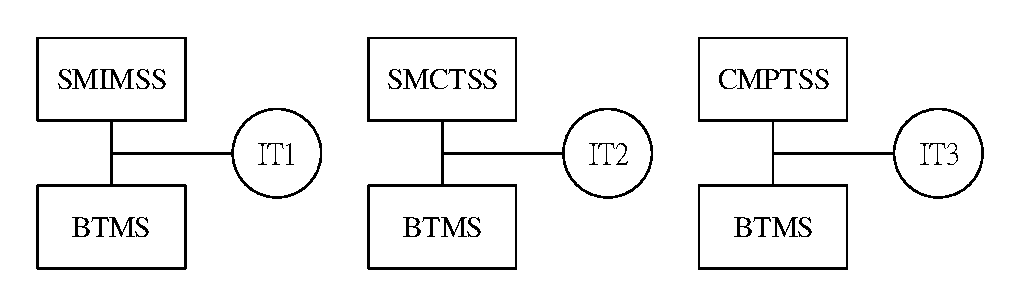
\includegraphics[width = 0.75\textwidth]{IntegrationTesting.pdf}
					\caption{集成子系统测试}\label{IntegrationTesting}
				\end{figure}
			\item 验收测试规划(Acceptance Testing,AT):
				本系统须达成以下三组接受用例陈列的所有功能,测试本论文设计与搭建的系统功能是否能够顺利运行。测试的角色有两个,分别为管理员以及用户,如图\ref{usecasediagram}为BTMS用例示意图,预计测试服务器的组态设置、手机的组态设置以及数据库的组态设置:

					\begin{figure}[!htbp]
						\centering
						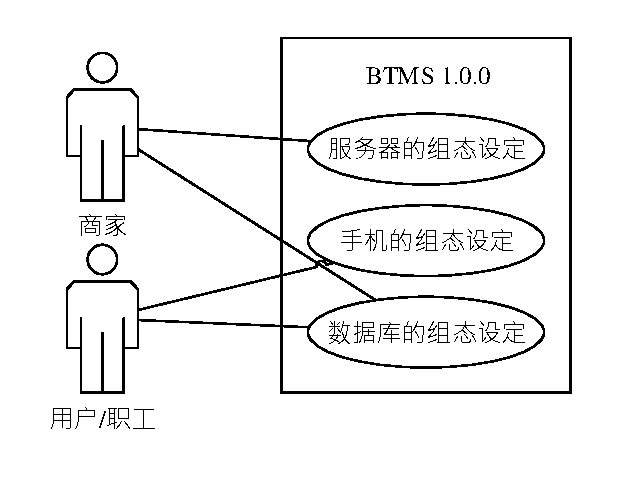
\includegraphics[width = 0.4\textwidth]{usecasediagram.pdf}
						\caption{BTMS用户用例图}\label{usecasediagram}
					\end{figure}

				图\ref{AcceptanceTesting}为三组验收测试的示意图,对本比特币的交易监督系统进行测试。
					\begin{figure}[!htbp]
						\centering
						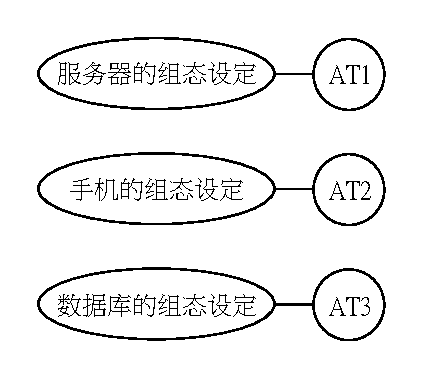
\includegraphics[width = 0.3\textwidth]{AcceptanceTesting.pdf}
						\caption{验收测试(Acceptance Testing)}\label{AcceptanceTesting}
					\end{figure}

	 		\end{enumerate}			

		\subsection{测试用例}
			\begin{enumerate}

			\item 集成测试(Integration Test):
				\begin{enumerate}

				\item IT1 测试用例:
					表\ref{IT1TestCase}为IT1 测试用例,测试对象为参与者商家装载于手机的商家和商品信息管理子系统(SMIMSS)的五项功能分别为添加店家帐户、添加/修改/删除职工帐户、添加/删除/修改商品信息、取得产品信息以及接收交易信息,上述SMIMSS的五项功能需与母系统BTMS交互,BRTMS皆以BTMS-F-001 的ID进行。目的:验证[SMIMSS 1.1.0]子系统能否正确管理商家商品信息。

					\begin{table}[!htbp]
					\centering
					\caption{IT1 测试用例}
					\label{IT1TestCase}
					\begin{tabular}{|l|l|}
					\hline
					用例ID & IT1 \\ \hline
					用例名称 & 集成SMIMSS至BTMS \\ \hline
					测试目标 & {[}BTMS 1.0.0{]}、{[}SMIMSS 1.1.0{]} \\ \hline
					依赖关系 & SMIMSS-F-001$\sim$ SMIMSS-F-005 \\ \hline
					严重程度 & 1(Critical) \\ \hline
					\multirow{5}{*}{用例描述} & 1.     能够添加店家帐户 \\ \cline{2-2} 
					 & 2.     能够添加/修改/删除职工帐户 \\ \cline{2-2} 
					 & 3.     能够添加/删除/修改商品信息 \\ \cline{2-2} 
					 & 4.     能够取得产品信息 \\ \cline{2-2} 
					 & 5.     能够接收交易信息 \\ \hline
					\multirow{5}{*}{预期结果} & 1.     成功添加店家帐户 \\ \cline{2-2} 
					 & 2.     成功添加/修改/删除职工帐户 \\ \cline{2-2} 
					 & 3.     成功添加/修改/删除商品信息 \\ \cline{2-2} 
					 & 4.     成功取得产品信息 \\ \cline{2-2} 
					 & 5.     成功接收交易信息 \\ \hline
					Cleanup & 无 \\ \hline
					\end{tabular}
					\end{table}


				\item IT2测试用例:
					表\ref{IT2TestCase}为IT2 测试用例目标,测试对象为装载于商家装载于商家职工Google Nexus 5X 手机的商家手持移动装置收款及交易子系统(SMCTSS),于IT2 应测试的SMCTSS 子系统的功能包括登入职工帐户、扫描RFID标签、读取商品信息、创建交易清单、发送交易信息、认证交易信息以及存储交易明细七项功能,上述七项功能需与母系统BTMS进行交互,BRTMS接受测试的ID 为BTMS-F-002。目的:验证[SMCTSS 1.2.0]子系统是否能够完成一笔行动支付之交易。

						\begin{table}[!htbp]
						\caption{IT2 测试用例} % title of Table
						\centering % used for centering table
						\label{IT2TestCase} % is used to refer this table in the text
						\begin{tabular}{|l|l|}
						\hline
						用例ID & IT2 \\ \hline
						用例名称 & 集成SMCTSS至BTMS \\ \hline
						测试目标 & {[}BTMS 1.0.0{]}、{[}SMCTSS 1.2.0{]} \\ \hline
						依赖关系 & SMCTSS-F-001$\sim$ SMCTSS-F-007 \\ \hline
						严重程度 & 1(Critical) \\ \hline
						\multirow{7}{*}{用例描述} & 1.     能够登入职工帐户 \\ \cline{2-2} 
						 & 2.     能够扫描RFID标签 \\ \cline{2-2} 
						 & 3.     能够读取商品信息 \\ \cline{2-2} 
						 & 4.     能够创建交易清单 \\ \cline{2-2} 
						 & 5.     能够发送交易信息 \\ \cline{2-2} 
						 & 6.     能够认证交易信息 \\ \cline{2-2} 
						 & 7.     能够存储交易明细 \\ \hline
						\multirow{7}{*}{预期结果} & 1.     成功登入职工帐户 \\ \cline{2-2} 
						 & 2.     成功扫描RFID标签 \\ \cline{2-2} 
						 & 3.     成功读取商品信息 \\ \cline{2-2} 
						 & 4.     成功创建交易清单 \\ \cline{2-2} 
						 & 5.     成功发送交易信息 \\ \cline{2-2} 
						 & 6.     成功认证交易信息 \\ \cline{2-2} 
						 & 7.     成功存储交易明细 \\ \hline
						Cleanup & 无 \\ \hline
						\end{tabular}
						\end{table}

				\item IT3测试用例:
					表\ref{IT3TestCase}为IT3 测试用例,目标测试对象为客户端行动支付和交易子系统(CMPTSS)的七项功能是否能够顺利运行,其功能包括登入顾客帐号、读取商品信息、接收交易清单、认证交易信息、运行行动支付、存储交易明细以及查看交易纪录,上述七项功能需与母系统BTMS进行交互,母系统于CMPTSS之间七项的功能性测试的ID为BTMS-F-003。目的:验证[CMPTSS 1.3.0]能正确接收SMCTSS所发送的交易数据,并以其交易信息运行以比特币付款之动作。可以查找商品信息,且能够存储并且查看用户过往之交易纪录。

						\begin{table}[!htbp]
						\caption{IT3 测试用例} % title of Table
						\centering % used for centering table
						\label{IT3TestCase} % is used to refer this table in the text
						\begin{tabular}{|l|l|}
						\hline
						用例ID & IT3 \\ \hline
						用例名称 & 集成CMPTSS至BTMS \\ \hline
						测试目标 & {[}BTMS 1.0.0{]}、{[}CMPTSS 1.3.0{]} \\ \hline
						依赖关系 & CMPTSS-F-001$\sim$ CMPTSS-F-007 \\ \hline
						严重程度 & 1(Critical) \\ \hline
						\multirow{7}{*}{用例描述} & 1.     能够登入顾客帐号 \\ \cline{2-2} 
						 & 2.     能够读取商品信息 \\ \cline{2-2} 
						 & 3.     能够接收交易清单 \\ \cline{2-2} 
						 & 4.     能够认证交易信息 \\ \cline{2-2} 
						 & 5.     能够运行行动支付 \\ \cline{2-2} 
						 & 6.     能够存储交易明细 \\ \cline{2-2} 
						 & 7.     能够查看交易纪录 \\ \hline
						\multirow{7}{*}{预期结果} & 1.     成功登入顾客帐号 \\ \cline{2-2} 
						 & 2.     成功读取商品信息 \\ \cline{2-2} 
						 & 3.     成功接收交易清单 \\ \cline{2-2} 
						 & 4.     成功认证交易信息 \\ \cline{2-2} 
						 & 5.     成功运行行动支付 \\ \cline{2-2} 
						 & 6.     成功存储交易纪录 \\ \cline{2-2} 
						 & 7.     成功查看交易纪录 \\ \hline
						Cleanup & 无 \\ \hline
						\end{tabular}
						\end{table}
				\end{enumerate}

		\item 验收测试用例(Acceptance Testing Cases):
			验收测试用例目的在于测试母系统BTMS、子系统SMIMSS、SMCTSS与CMPTSS是否能够顺利的进行信息传递完成交互。

			\begin{enumerate}
				\item AT1 测试用例:
					表\ref{AT1TestCase}所示,目标测试管理人员是否能够顺利使用子系统SMIMSS顺利与母系统BTMS交互。目的:验证使用用例(Use case)1,透过组态文件的修改对服务器进行组态设置。

						\begin{table}[!htbp]
						\centering
						\caption{AT1 测试用例}
						\label{AT1TestCase}
						\begin{tabular}{|l|l|l|}
						\hline
						用例ID & \multicolumn{2}{l|}{AT1} \\ \hline
						用例名称 & \multicolumn{2}{l|}{服务器的组态设置} \\ \hline
						测试目标 & \multicolumn{2}{l|}{\begin{tabular}[c]{@{}l@{}}{[}SMIMSS 1.1.0{]}\\ {[}BTMS 1.0.0{]}\end{tabular}} \\ \hline
						依赖关系 & \multicolumn{2}{l|}{BTMS-F-001} \\ \hline
						严重程度 & \multicolumn{2}{l|}{1(Critical)} \\ \hline
						\multirow{3}{*}{用例描述} & 用户操作 & 系统响应 \\ \cline{2-3} 
						 & \begin{tabular}[c]{@{}l@{}}1.管理人员依照环境\\    设置服务器组态。\end{tabular} &  \\ \cline{2-3} 
						 &  & \begin{tabular}[c]{@{}l@{}}2.服务器依照管理人\\    员所做的组态设置\\    启动服务。\end{tabular} \\ \hline
						预期结果 & \multicolumn{2}{l|}{成功启动服务器的相关服务。} \\ \hline
						Cleanup & \multicolumn{2}{l|}{无} \\ \hline
						\end{tabular}
						\end{table}

				\item AT2 测试用例:
					如表\ref{AT2TestCase}所示,参与者为用户。目的:验证用例(Use case )2 透过组态文件的修改对手机进行组态设置。
						\begin{table}[!htbp]
						\centering
						\caption{AT2 测试用例}
						\label{AT2TestCase}
						\begin{tabular}{|l|l|l|}
						\hline
						用例ID & \multicolumn{2}{l|}{AT2} \\ \hline
						用例名称 & \multicolumn{2}{l|}{手机的组态设置} \\ \hline
						测试目标 & \multicolumn{2}{l|}{\begin{tabular}[c]{@{}l@{}}{[}SMCTSS 1.2.0{]}\\ {[}CMPTSS 1.3.0{]}\end{tabular}} \\ \hline
						依赖关系 & \multicolumn{2}{l|}{BTMS-F-002$\sim$ BTMS-F-003} \\ \hline
						严重程度 & \multicolumn{2}{l|}{1(Critical)} \\ \hline
						\multirow{3}{*}{用例描述} & 用户操作 & 系统响应 \\ \cline{2-3} 
						 & \begin{tabular}[c]{@{}l@{}}1.用户修改手机组\\    态设置参数。\end{tabular} &  \\ \cline{2-3} 
						 &  & \begin{tabular}[c]{@{}l@{}}2.手机依照用户在\\    设置档中所填入的\\    数值运作。\end{tabular} \\ \hline
						预期结果 & \multicolumn{2}{l|}{成功完成手机的组态设置} \\ \hline
						Cleanup & \multicolumn{2}{l|}{无} \\ \hline
						\end{tabular}
						\end{table}

				\item AT3 测试用例:
					如表\ref{AT3TestCase}所示,目的:验证用例(Use case )3,透过组态文件的修改对数据库进行组态设置。

						\begin{table}[!htbp]
						\centering
						\caption{AT3 测试用例}
						\label{AT3TestCase}
						\begin{tabular}{|l|l|l|}
						\hline
						用例ID & \multicolumn{2}{l|}{AT3} \\ \hline
						用例名称 & \multicolumn{2}{l|}{数据库的组态设置} \\ \hline
						测试目标 & \multicolumn{2}{l|}{\begin{tabular}[c]{@{}l@{}}{[}SMIMSS 1.1.0{]}\\ {[}SMCTSS 1.2.0{]}\\ {[}CMPTSS 1.3.0{]}\end{tabular}} \\ \hline
						依赖关系 & \multicolumn{2}{l|}{BTMS-F-001$\sim$ BTMS-F-003} \\ \hline
						严重程度 & \multicolumn{2}{l|}{1(Critical)} \\ \hline
						\multirow{5}{*}{用例描述} & 用户操作 & 系统响应 \\ \cline{2-3} 
						 & \begin{tabular}[c]{@{}l@{}}1.管理者设置数据库\\    组态。\end{tabular} &  \\ \cline{2-3} 
						 &  & \begin{tabular}[c]{@{}l@{}}2.数据库依照管理人\\    员所做的组态设置\\    启动服务。\end{tabular} \\ \cline{2-3} 
						 & \begin{tabular}[c]{@{}l@{}}3.用户修改数据库\\    之数据及文件。\end{tabular} &  \\ \cline{2-3} 
						 &  & \begin{tabular}[c]{@{}l@{}}4.数据库依照用户\\    所做的组态设置启\\    动服务。\end{tabular} \\ \hline
						预期结果 & \multicolumn{2}{l|}{成功设置完成数据库的相关设置。} \\ \hline
						Cleanup & \multicolumn{2}{l|}{无} \\ \hline
						\end{tabular}
						\end{table}
			\end{enumerate}
		\end{enumerate}

		\subsection{测试结果和分析}
		\begin{enumerate}

			\item 集成测试用例(Integration Testing Cases):其中IT1测试对象为装载于Windows 10 主机中的BTMS系统与装在于商家Windows 10 主机的SMIMSS子系统,当中测试用户商家在操作以Java 编成语言实现的商家和商品信息子系统时所使用到的每一像功能,包括添加店家帐户、添加/修改/删除职工帐户、添加/删除/修改商品信息、取得产品信息以及接收交易信息,在IT1 的功能测试中都能够顺利运行。IT2 测试对象为装载于Windows 10 的BTMS 系统与装载于商家职工Google Nexus 5X 手机的SMCTSS子系统,测试功能包括登入职工帐户、扫描RFID 标签、读取商品信息、创建交易清单、发送交易信息、认证交易信息以及存储交易明细的功能,在功能测试的结果中显示,上述功能皆可顺利运行。在IT3 功能性测试中,测试对象为装载于Windows 10 的BTMS 系统以及装载于顾客小米 3 手机的CMPTSS 子系统,测试功能包括登入顾客帐号、读取商品信息、接收交易清单、认证交易信息、运行行动支付、存储交易明细以及查看交易纪录,于测试结果中显示上述功能皆能顺利运行。
			表\ref{table8}为IT1、为IT2、为IT3的集成子系统测试结果,皆顺利运作。

				\begin{table}[!htbp]
				\centering
				\caption{集成子系统测试结果}
				\label{table8}
				\begin{tabular}{|c|c|l|}
				\hline
				测试用例 & 结果 (通过/不通过) & Comment \\ \hline
				\multirow{5}{*}{IT1} & \multirow{5}{*}{通过} & 1.成功添加店家帐户 \\ \cline{3-3} 
				 &  & 2.成功添加/修改/删除职工帐户 \\ \cline{3-3} 
				 &  & 3.成功添加/修改/删除商品信息 \\ \cline{3-3} 
				 &  & 4.成功取得产品信息 \\ \cline{3-3} 
				 &  & 5.成功接收交易信息 \\ \hline
				\multirow{7}{*}{IT2} & \multirow{7}{*}{通过} & 1.成功登入职工帐户 \\ \cline{3-3} 
				 &  & 2.成功扫描RFID标签 \\ \cline{3-3} 
				 &  & 3.成功读取商品信息 \\ \cline{3-3} 
				 &  & 4.成功创建交易清单 \\ \cline{3-3} 
				 &  & 5.成功发送交易信息 \\ \cline{3-3} 
				 &  & 6.成功认证交易信息 \\ \cline{3-3} 
				 &  & 7.成功存储交易明细 \\ \hline
				\multirow{7}{*}{IT3} & \multirow{7}{*}{通过} & 1.成功登入顾客帐号 \\ \cline{3-3} 
				 &  & 2.成功读取商品信息 \\ \cline{3-3} 
				 &  & 3.成功接收交易清单 \\ \cline{3-3} 
				 &  & 4.成功认证交易信息 \\ \cline{3-3} 
				 &  & 5. 成功运行行动支付 \\ \cline{3-3} 
				 &  & 6.成功存储交易纪录 \\ \cline{3-3} 
				 &  & 7.成功查看交易纪录 \\ \hline
				RATE & 100\% & \begin{tabular}[c]{@{}l@{}}\\ \\ \\ \\ \\ \\ \end{tabular} \\ \hline
				\end{tabular}
				\end{table}

			\item 验收测试用例(Acceptance Testing Cases):在AT1 中
			表\ref{table9}为前节所设计的三种AT1、AT2与AT3的验收测试结果,皆顺利运行。
				\begin{table}[!htbp]
				\centering
				\caption{验收测试结果}
				\label{table9}
				\begin{tabular}{|c|c|l|}
				\hline
				测试用例 & 结果(通过/不通过) & Comment \\ \hline
				AT1 & 通过 & 成功启动服务器的相关服务。 \\ \hline
				AT2 & 通过 & 成功完成手机的组态设置。 \\ \hline
				AT3 & 通过 & 成功设置完成数据库的相关设置。 \\ \hline
				RATE & 100\% & \begin{tabular}[c]{@{}l@{}}BTMS可透过组态设置的方式来设\\ 定各个子系统的环境参数。\end{tabular} \\ \hline
				\end{tabular}
				\end{table}
						\begin{table}[!htbp]
						\centering
						\caption{子系统与测试用例关系表}
						\label{table10}
						\begin{tabular}{|l|c|c|c|}
						\hline
						 & \multicolumn{1}{l|}{SMIMSS 1.1.0} & \multicolumn{1}{l|}{SMCTSS 1.2.0} & \multicolumn{1}{l|}{CMPISS 1.3.0} \\ \hline
						IT1 & X &  &  \\ \hline
						IT2 &  & X &  \\ \hline
						IT3 &  &  & X \\ \hline
						AT1 & X &  &  \\ \hline
						AT2 &  & X & X \\ \hline
						AT3 & X & X & X \\ \hline
						\end{tabular}
						\end{table}

						\begin{table}[!htbp]
					\centering
					\caption{需求与集成测试用例的关系表}
					\label{table11}
					\begin{tabular}{|c|c|c|c|c|}
					\hline
					ID & 描述 & IT1 & IT2 & IT3 \\ \hline
					BTMS-F-001 & 接收SMIMSS信息 & X &  &  \\ \hline
					BTMS-F-002 & 接收SMCTSS信息 &  & X &  \\ \hline
					BTMS-F-003 & 接收CMPTSS信息 &  &  & X \\ \hline
					SMIMSS-F-001 & 添加店家帐户 & X &  &  \\ \hline
					SMIMSS-F-002 & 添加/修改/删除职工帐户 & X &  &  \\ \hline
					SMIMSS-F-003 & 添加/修改/删除商品信息 & X &  &  \\ \hline
					SMIMSS-F-004 & 取得产品信息 & X &  &  \\ \hline
					SMIMSS-F-005 & 接收交易信息 & X &  &  \\ \hline
					SMCTSS-F-001 & 登入职工帐户 &  & X &  \\ \hline
					SMCTSS-F-002 & 扫描 RFID 标签 &  & X &  \\ \hline
					SMCTSS-F-003 & 读取商品信息 &  & X &  \\ \hline
					SMCTSS-F-004 & 创建交易清单 &  & X &  \\ \hline
					SMCTSS-F-005 & 发送交易信息 &  & X &  \\ \hline
					SMCTSS-F-006 & 认证交易信息 &  & X &  \\ \hline
					SMCTSS-F-007 & 存储交易明细 &  & X &  \\ \hline
					CMPTSS-F-001 & 登入顾客帐号 &  &  & X \\ \hline
					CMPTSS-F-002 & 读取商品信息 &  &  & X \\ \hline
					CMPTSS-F-003 & 接收交易清单 &  &  & X \\ \hline
					CMPTSS-F-004 & 认证交易信息 &  &  & X \\ \hline
					CMPTSS-F-005 & 运行行动支付 &  &  & X \\ \hline
					CMPTSS-F-006 & 存储交易纪录 &  &  & X \\ \hline
					CMPTSS-F-007 & 查看交易纪录 &  &  & X \\ \hline
					\end{tabular}
					\end{table}


					\begin{table}[!htbp]
					\centering
					\caption{需求与验收测试案例的关系表}
					\label{table12}
					\begin{tabular}{|l|c|c|c|}
					\hline
					 & \multicolumn{1}{l|}{AT1} & \multicolumn{1}{l|}{AT2} & \multicolumn{1}{l|}{AT3} \\ \hline
					BTMS-F-001 & X &  & X \\ \hline
					BTMS-F-002 &  & X & X \\ \hline
					BTMS-F-003 &  & X & X \\ \hline
					\end{tabular}
					\end{table}


			\item 可追踪性(Traceability)

						

			\begin{enumerate}
				\item 子系统与测试用例:表\ref{table10}为测试组IT1、IT2、IT3、AT1、AT2、AT3与子系统SMIMSS、SMCTSS、CMPISS的关系表。
				\item 需求与测试用例:表\ref{table11}为本系统需求与集成测试用例的关系表,表\ref{table12}为需求与验收测试案例的关系表。
				\end{enumerate}
		\end{enumerate}

	BTMS开发透过手机让商家及顾客以手机发送交易信息,如:商品名称、商品金额,商家收款地址。并且及时将商品信息更新至服务器之数据库,以便商家控管商品信息状态,同时让顾客可以享受数字加密货币的方便性。

	\section{性能测试}


		\begin{figure}[!htbp]
			\centering
			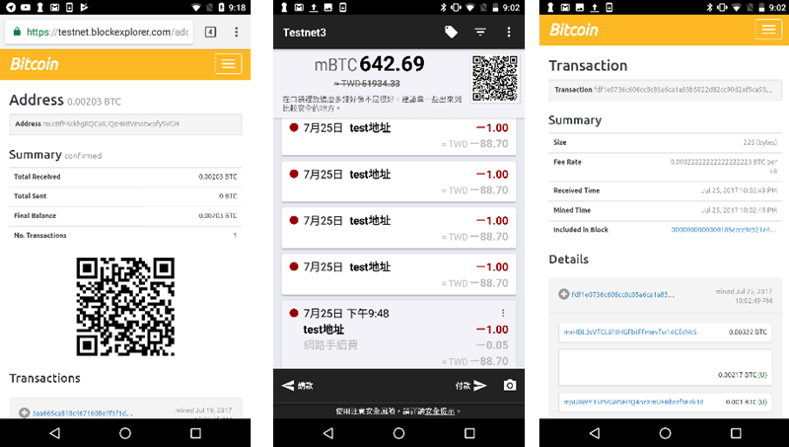
\includegraphics[width = 0.8\textwidth]{fig9.png}
			\caption{使用区块链检视器验证存储在比特币区块链中的交易过程}\label{fig9}
		\end{figure}


		根据比特币点对点架构,尽管顾客和商家之间的交易细节已经快速存储到云数据库,但官方确认交易与当前比特币区块链的交易通常需要更长的时间,因为需要确保确认的数量在交易广播比特币点对点网络并存储到缓存池后,是否存在双重支付。本文设计了比特币的交易监督系统以及引用多重签章算法重新设计的比特币的实时交易监督系统,以下将分别针对有无采用多重签章算法的性能测试。


		\subsection{系统性能测试}
		为了验证本文提出的BTMS不会通过使用比特币等加密货币影响交易完成时间,于2017年7月25日、2017年9月6日以及2018年3月21日,在Testnet实验中连续记录了20笔交易信息,每1秒发出一笔交易,分别历时20分钟。

		\begin{enumerate}
			\item 初始测试(2017年7月25日):
			首先,使用区块链检视器(Blockchain Explorer)\supercite{Blockchainexplorer:Ananalyticalprocessandinvestigationenvironmentforbitcoin},如图\ref{fig9}的快照所示,透过使用Testnet依序进行20笔比特币交易,如图\ref{fig9}的中间快照所示,最后20笔交易完成时间全部记录在区块链检视器。实验结果显示,实验中的所有交易都在3秒钟左右(平均2.97秒,标准差小于1秒)发送到比特币网络缓存池,平均交易完成时间在比特币区块链中确认为522.33秒(小于9分钟),标准差大约为339秒。

			\item 第一次测试结果与分析(2017年9月6日):表\ref{1general}为第一次实验数据,该次的比特币交易发起广播至比特币交易缓存池的时间平均为1.918秒,标准差为0.55586秒。但为了预防双重支付攻击需要等待平均654.8秒(小于11分钟,标准差346.63秒)的时间。

				\begin{table}[!htbp]
				\centering
				\caption{第一次Testnet 运行实验之数据分析(2017年9月6日)}
				\label{1general}
				\begin{tabular}{|c|c|c|c|}
				\hline
				         & 进入缓存池时间(秒) & 进入区块链时间(秒)    & 完成交易时间(秒)     \\ \hline
				平均       & 1.918      & 654.8         & 654.8         \\ \hline
				样本标准差    & 0.55586    & 346.63        & 346.63        \\ \hline
				95\%信赖区间 & 1.69~2.15  & 511.72~797.88 & 511.72~797.88 \\ \hline
				99\%信赖区间 & 1.61~2.23  & 460.9~848.7   & 460.9~848.7   \\ \hline
				\end{tabular}
				\end{table}

			\item 第二次测试结果与分析(2018年3月21日):表\ref{2general}为第二次测试的实验原始数据,表\ref{2general-1}为将数据进行分析后的结果可以看出,平均进入缓存池的时间为1.12秒,进入区块链的时间为287.12秒,因为并未采用多重签章算法,所以交易完成时间以287.12秒计算。
				\begin{table}[!htbp]
				\centering
				\caption{第二次Testnet 运行实验数据(2018年3月21日)}
				\label{2general}
				\begin{tabular}{|c|c|c|c|c|c|}
				\hline
				\begin{tabular}[c]{@{}c@{}}交易\\ 次数\end{tabular} & 付款时间 & \begin{tabular}[c]{@{}c@{}}进入缓存池\\ 所花时间(秒)\end{tabular} & \begin{tabular}[c]{@{}c@{}}进入缓存池\\ 时间点\end{tabular} & \begin{tabular}[c]{@{}c@{}}写入区块链\\ 所花时间(秒)\end{tabular} & \begin{tabular}[c]{@{}c@{}}写入区块\\ 时间点\end{tabular} \\ \hline
				1 & 0:00:00 & 3 & 0:00:03 & 136 & 0:02:16 \\ \hline
				2 & 0:01:00 & 1 & 0:01:01 & 76 & 0:02:16 \\ \hline
				3 & 0:02:04 & 3 & 0:02:07 & 12 & 0:02:16 \\ \hline
				4 & 0:03:00 & 1 & 0:03:01 & 438 & 0:10:18 \\ \hline
				5 & 0:04:00 & 1 & 0:04:01 & 378 & 0:10:18 \\ \hline
				6 & 0:05:00 & 1 & 0:05:01 & 318 & 0:10:18 \\ \hline
				7 & 0:06:00 & 2 & 0:06:02 & 258 & 0:10:18 \\ \hline
				8 & 0:07:00 & 1 & 0:07:01 & 198 & 0:10:18 \\ \hline
				9 & 0:08:00 & 1 & 0:08:01 & 138 & 0:10:18 \\ \hline
				10 & 0:09:00 & 1 & 0:09:01 & 78 & 0:10:18 \\ \hline
				11 & 0:10:00 & 1 & 0:10:01 & 18 & 0:10:18 \\ \hline
				12 & 0:11:00 & 2 & 0:11:02 & 810 & 0:24:30 \\ \hline
				13 & 0:12:00 & 1 & 0:12:01 & 750 & 0:24:30 \\ \hline
				14 & 0:13:00 & 1 & 0:13:01 & 690 & 0:24:30 \\ \hline
				15 & 0:14:00 & 1 & 0:14:01 & 630 & 0:24:30 \\ \hline
				16 & 0:15:00 & 1 & 0:15:01 & 570 & 0:24:30 \\ \hline
				17 & 0:16:00 & 2 & 0:16:02 & 510 & 0:24:30 \\ \hline
				18 & 0:17:00 & 2 & 0:17:02 & 450 & 0:24:30 \\ \hline
				19 & 0:18:00 & 1 & 0:18:01 & 390 & 0:24:30 \\ \hline
				20 & 0:19:00 & 1 & 0:19:01 & 330 & 0:24:30 \\ \hline
				\end{tabular}
				\end{table}

				\begin{table}[!htbp]
				\centering
				\caption{第二次以Testnet 运行实验数据分析(2018年3月21日)}
				\label{2general-1}
				\begin{tabular}{|c|c|c|c|}
				\hline
				         & 进入缓存池时间(秒) & 进入区块链时间(秒)    & 完成交易时间(秒)     \\ \hline
				平均       & 1.12       & 287.12        & 287.12        \\ \hline
				样本标准差    & 0.68       & 246.59        & 246.59        \\ \hline
				95\%信赖区间 & 0.84~1.4   & 185.33~388.91 & 185.33~388.91 \\ \hline
				99\%信赖区间 & 0.74~1.5   & 149.18~425.06 & 149.18~425.06 \\ \hline
				\end{tabular}
				\end{table}


		\end{enumerate}

			在未引用多重签章算法的监督系统中,第一次与第二次的测试相比并无太大的差异,交易完成时间与比特币区块生成所需时间相同,平均时间皆为十分钟。根据比特币Testnet上的初步实验结果显示,本文提出的BTMS可以快速有效地运行比特币的交易监督系统。

			%

		\subsection{实时系统性能测试}
		本节介绍比特币测试币于Government Green Address钱包进行交易的性能实验与结果分析,包含该实验的目的、方法及结果分析。实验的目的是要确认的系统在商家端进行行动支付时能快速、精准且高效率的进行交易,并了解使用一般Testnet钱包与Government Green Address钱包作为交易媒介的确认交易时间的差距。表\ref{0test}为2017年7月25日初步的采用多重签章算法的测试数据,数据显示交易存储到区块链的平均时间为10分钟,但Government Green Address采用的多重签章算法,可以有效拒绝双重花费的交易发起,因此可将交易的有效时间,从交易进入区块链的时间,重新订定为交易进入比特币交易缓存池的时间。

		\begin{table}[!htbp]
			\centering
			\caption{初步的Government Green Address实验测试数据 (2017年7月25日)}
			\label{0test}
			\begin{tabular}{|c|c|c|c|c|}
			\hline
			\multicolumn{1}{|c|}{付款时间} & \multicolumn{1}{c|}{\begin{tabular}[c]{@{}c@{}}进入缓存池\\ 所花时间(秒)\end{tabular}} & \multicolumn{1}{c|}{\begin{tabular}[c]{@{}c@{}}进入缓存池\\ 时间点\end{tabular}} & \multicolumn{1}{c|}{入块时间} & \multicolumn{1}{c|}{\begin{tabular}[c]{@{}c@{}}写入区块\\ 费时间\end{tabular}} \\ \hline
			06:36:25 & 2.14 & 06:36:27.14 & 06:52:00 & 16:25 \\ \hline
			06:38:25 & 1.075 & 06:38:26.075 & 06:52:00 & 14:25 \\ \hline
			06:40:25 & 1.722 & 06:40:26.722 & 06:52:00 & 12:25 \\ \hline
			06:42:25 & 2.953 & 06:42:27.953 & 06:52:00 & 10:25 \\ \hline
			06:44:25 & 1.511 & 06:44:26.511 & 06:52:00 & 08:25 \\ \hline
			06:46:25 & 2.269 & 06:46:27.269 & 06:52:00 & 06:25 \\ \hline
			06:48:25 & 1.831 & 06:48:26.831 & 06:52:00 & 04:25 \\ \hline
			06:50:25 & 1.227 & 06:50:26.227 & 06:52:00 & 02:25 \\ \hline
			06:52:25 & 2.026 & 06:52:27.026 & 07:12:01 & 20:24 \\ \hline
			06:54:25 & 1.257 & 06:54:26.257 & 07:12:01 & 18:24 \\ \hline
			06:56:25 & 1.511 & 06:56:26.511 & 07:12:01 & 16:24 \\ \hline
			06:58:25 & 2.815 & 06:58:27.815 & 07:12:01 & 14:24 \\ \hline
			07:00:26 & 1.544 & 07:00:27.544 & 07:12:01 & 12:25 \\ \hline
			07:02:25 & 1.767 & 07:02:26.767 & 07:12:01 & 10:24 \\ \hline
			07:04:25 & 1.52 & 07:04:26.52 & 07:12:01 & 08:24 \\ \hline
			07:06:25 & 1.953 & 07:06:26.953 & 07:12:01 & 06:24 \\ \hline
			\end{tabular}
			\end{table}


		本次的实验分为两部份,分别是透过比特币 Testnet钱包以及使用本论文所采用的Government Green Address比特币钱包上运行20次付款,皆以相同地址收款,交易金额都设置为0.00001 BTC,实验时间为2017年9月6日与2018年2月6日,每隔一分钟运行一次付款的动作,总共历时20分钟。两款钱包同时发起交易,并透过区块链检视器进行记录时间,最后再比较使用一般比特币钱包及Government Green Address钱包两者之间的差距。

		\begin{enumerate}
			\item 第一次测试结果与分析(2017年9月6日):表\ref{1green}为第一次测试实验的数据分析结果,平均进入交易缓存池的时间为2.11秒,真正写入区块链的时间为654.24秒,采用多重签章算法,这些交易不存在双重支付的问题,因此完成时间记为2.11秒。

			\begin{table}[!htbp]
				\centering
				\caption{第一次以Government Green Address运行实验之数据分析(2017年9月6日)}
				\label{1green}
				\begin{tabular}{|c|c|c|c|}
				\hline
				         & 进入缓存池时间(秒) & 进入区块链时间(秒)    & 完成交易时间(秒) \\ \hline
				平均       & 2.11       & 654.24        & 2.11      \\ \hline
				样本标准差    & 0.65       & 346.9         & 0.65      \\ \hline
				95\%信赖区间 & 1.84~2.38  & 511.05~797.43 & 1.84~2.38 \\ \hline
				99\%信赖区间 & 1.75~2.47  & 460.19~848.29 & 1.75~2.47 \\ \hline
				\end{tabular}
				\end{table}

			\item 第二次测试结果与分析(2018年3月21日):表\ref{2green}为第二次以Government Green Address运行实验数据,表\ref{2green-1}为基于第二次测试的数据分析结果,进入缓存池的平均时间为1.55秒,进入区块链的平均时间为431.4秒,因为采用多重签章算法将完成交易时间以1.55秒计算。

		\end{enumerate}
			\begin{table}[!htbp]
				\centering
				\caption{第二次以Government Green Address运行实验数据(2018年3月21日)}
				\label{2green}
				\begin{tabular}{|c|c|c|c|c|c|}
				\hline
				\begin{tabular}[c]{@{}c@{}}交易\\ 次数\end{tabular} & 付款时间 & \begin{tabular}[c]{@{}c@{}}进入缓存池\\ 所花时间(秒)\end{tabular} & \begin{tabular}[c]{@{}c@{}}进入缓存池\\ 时间点\end{tabular} & \begin{tabular}[c]{@{}c@{}}写入区块链\\ 所花时间(秒)\end{tabular} & \begin{tabular}[c]{@{}c@{}}写入区块\\ 时间点\end{tabular} \\ \hline
				1 & 0:00:01 & 2 & 0:00:03 & 619 & 0:10:18 \\ \hline
				2 & 0:01:00 & 1 & 0:01:01 & 559 & 0:10:18 \\ \hline
				3 & 0:02:02 & 2 & 0:02:04 & 496 & 0:10:18 \\ \hline
				4 & 0:03:00 & 1 & 0:03:01 & 438 & 0:10:18 \\ \hline
				5 & 0:04:00 & 1 & 0:04:01 & 378 & 0:10:18 \\ \hline
				6 & 0:05:00 & 2 & 0:05:02 & 318 & 0:10:18 \\ \hline
				7 & 0:06:00 & 1 & 0:06:01 & 258 & 0:10:18 \\ \hline
				8 & 0:07:00 & 1 & 0:07:01 & 198 & 0:10:18 \\ \hline
				9 & 0:08:00 & 2 & 0:08:02 & 138 & 0:10:18 \\ \hline
				10 & 0:09:00 & 2 & 0:09:02 & 78 & 0:10:18 \\ \hline
				11 & 0:10:00 & 1 & 0:10:01 & 18 & 0:10:18 \\ \hline
				12 & 0:11:00 & 2 & 0:11:02 & 810 & 0:24:30 \\ \hline
				13 & 0:12:00 & 2 & 0:12:02 & 750 & 0:24:30 \\ \hline
				14 & 0:13:00 & 1 & 0:13:01 & 690 & 0:24:30 \\ \hline
				15 & 0:14:00 & 2 & 0:14:02 & 630 & 0:24:30 \\ \hline
				16 & 0:15:00 & 1 & 0:15:01 & 570 & 0:24:30 \\ \hline
				17 & 0:16:00 & 2 & 0:16:02 & 510 & 0:24:30 \\ \hline
				18 & 0:17:00 & 2 & 0:17:02 & 450 & 0:24:30 \\ \hline
				19 & 0:18:00 & 1 & 0:18:01 & 390 & 0:24:30 \\ \hline
				20 & 0:19:00 & 2 & 0:19:02 & 330 & 0:24:30 \\ \hline
				\end{tabular}
				\end{table}

			\begin{table}[!htbp]
				\centering
				\caption{第二次以Government Green Address运行实验之数据分析(2018年3月21日)}
				\label{2green-1}
				\begin{tabular}{|c|c|c|c|}
				\hline
				         & 进入缓存池时间(秒)     & 进入区块链时间(秒)         & 完成交易时间(秒)      \\ \hline
				平均       & 1.55           & 431.4              & 1.55           \\ \hline
				样本标准差    & 0.51           & 220.84             & 0.51           \\ \hline
				95\%信赖区间 & 1.34$\sim$1.76 & 340.24$\sim$522.56 & 1.34$\sim$1.76 \\ \hline
				99\%信赖区间 & 1.26$\sim$1.84 & 307.86$\sim$554.94 & 1.26$\sim$1.84 \\ \hline
				\end{tabular}
				\end{table}

				

				
				

	%			\begin{figure}[!htbp]
	%				\centering
	%				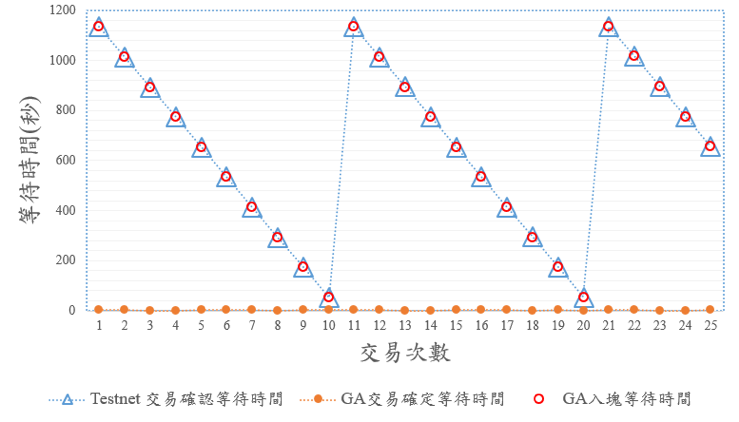
\includegraphics[width = 0.7\textwidth]{fig12.png}
	%				\caption{fig12}\label{fig12}
	%

%				\end{figure}

	本次实验分别记录以Testnet钱包及Government Green Address钱包运行20次交易的进入缓存池等待时间和写入区块等待时间。若以Testnet钱包交易,必须等到交易写入才能保证此笔交易不会被矿工遗弃,也才算真的完成这笔交易;但若以Government Green Address钱包发起交易就大不相同,当交易进入缓存池,即使遇到交易被矿工遗弃的情况,Government Green Address机构节点也会重新发起此笔交易,保证让交易写入区块,所以只要进入缓存池就可以视为交易完成,透过两者钱包的交易数据,本文分析两种钱包交易的时间数据。

	\begin{table}[!htbp]
	\centering
	\caption{原始系统与实时系统比较表}
	\label{generalvsga}
	\begin{tabular}{|c|c|}
	\hline
	 & 完成交易时间(秒) \\ \hline
	原始系统(BTMS)交易平均时间 & 287.12 \\ \hline
	实时系统(BRTMS)交易平均时间 & 1.55 \\ \hline
	\end{tabular}
	\end{table}

	透过本次的实验可以发现虽然以两种钱包交易进入区块的等待时间完全相同,但因为Government Green Address钱包的特性,只要进入缓存池就算完成交易确认,因此Government Green Address钱包的完成交易确认的时间远远快于一般Testnet。相信以此⽅式作为主要⽀付管道,可以省去顾客在现金⽀付时掏零钱、算钱及找零等繁琐的动作及时间,以此达成提升⽇常⽣活中的便利性与安全性。



		
	  
\chapter{总结与展望}
设计并实现一个名为BRTMS(Bitcoin Realtime Transaction Monitoring System)的比特币的实时交易监督系统,其工作包括背景调研比特币技术上的优势与劣势、匿名交易衍生出无法保障顾客权益、政府无法课征税收及存在着透过比特币洗钱的问题。为解决上述问题,在技术调研方面针对比特币地址的相关算法、地址的生成过程、多重签章算法以及区块链技术进行剖析。设计系统之前得进行详细的需求分析以及交易模型分析。设计BRTMS时,加入Government Green Address使该系统成为实时监督系统,并实现BTMS与BRTMS的客户端与服务器端,最后对BTMS进行功能性测试和性能测试。性能测试的成果中可知BRTMS比BTMS(BitcoinTransaction Monitoring System)的交易完成时间从平均287.12秒缩减至1.55秒,达到更好的顾客消费体验。

在BRTMS中,顾客交易信息是匿名且公开透明,同时保障顾客消费权益;商家可以根据所有数字化交易信息为自己的业务目的进行统计和计算,减少手动操作计算结果中的错误。统计数据甚至可以与商家的库存管理相结合,使货物和资金更加便利地进行统计,进一步改善信息的准确性和降低人工成本;政府在解决交易纠纷的过程中拥有更多可信的证据供参考。数字交易交易凭据也可以解决纸本交易凭据丢失或破损的问题。本文提出的BRTMS架构包括以下特色如下:
		\begin{enumerate}
			\item 引入匿名支付给实名的交易模型至加密货币交易系统。
			\item 设计与实现于加密货币中匿名支付给实名的交易监督系统。
			\item 于政府端实现多重签章算法,使实时的交易监督比Green Address节点更快速。
			\item 透过多重签章算法使得商家可以预防双重支付攻击。
			\item 商家商品管理让商家可进行库存管理及商家商品管理。
			\item 实现于加密货币中,消费者匿名同时也让消费者拥有消费者权益。
			\item 借由将商家实名,BRTMS使政府主管机关可以有效获得税收。
		\end{enumerate}



		
BRTMS不仅兼顾顾客和商家同时协助府金融监督单位审计加密货币交易筹集税收。本系统中以bitcoinj库实作的Java应用程序和Android应用程序客户端,修改其在Android系统上的开放源代码应用程序,使得本论文阐述之概念能够实际在区块链上运行,未来加密货币不仅能维持目前的便利性,还可以让用户不用担心交易后找不到卖家,使一般民众能更安心使用加密货币作为日常生活的行动支付管道。

%	% Copyright (c) 2014,2016 Casper Ti. Vector
% Public domain.

\chapter{結論}
在本文中,我們建議並實施一個名為BRTMS的区块链实名交易监督系统,不僅為分別花錢和賺取加密貨幣的客戶和商家,同時也能協助府金融監督單位審計加密貨幣交易籌集稅收。 此外,加密貨幣交易實驗的初步結果,使用著名的Testnet比特幣和雲數據庫,我們以著名的比特幣加密貨幣錢包實作的Java應用程序和Android應用程序客戶端。
	
此外,修改其在Android系統上的開放原始碼應用程式,使得本論文闡述之概念能夠實際在區塊鏈上運行,以期未來加密貨幣不僅能維持目前的便利性,更能夠能避免不肖人士利用加密貨幣洗錢,還可以讓使用者不用擔心交易後找不到賣家,使一般民眾能更安心使用加密貨幣作為日常生活的行動支付管道。

	\section{提出的BRTMS架構還包括以下特色}

		\begin{enumerate}
			\item 向建議的BRTMS進行商業註冊需經政府批准。
			\item 所有出售的商品將受到政府審查。
			\item 消費者仍然匿名以確保個人信息的隱私。
			\item 消費者的交易記錄不能被刪除。
			\item 如果消費者有關交易上訴的問題,他們需要提交交易發票或證明付款人或收款人地址的訪問權。
			\item 所有交易記錄均公開透明。
			\item 原始交易數據採用區塊鏈技術記錄,具有高度的可靠性,分散和未篡改的數據。
			\item 政府可以檢查建議的BRTMS系統的交易記錄,以快速有效的方式審查稅務信息。
		\end{enumerate}

	\section{提議的BRTMS的優點總結}

		\paragraph{消費者}交易信息公開透明,保護消費者的權益。由於交易是可信的,並有明確的時間戳。當消費者需要上交他們的消費者權利時,他們可以從提出的系統中獲得更有效和可信的證據。
		\paragraph{商家}企業可以根據所有數字化交易信息為自己的業務目的進行統計和計算。這可以減少手動操作計算結果中的錯誤。統計數據甚至可以與商店的庫存管理相結合,使貨物和資金達到更加便利地進行統計,進一步改善業務的會計準確性和人工成本。
		\paragraph{政府}在解決交易糾紛的過程中,可以提供更多可信的證據供參考。數字交易收據也可以解決紙本收據丟失或破損的問題。考慮到稅收問題,政府可以審查具有高信譽的商業交易細節作為稅收計算程序,以定制徵稅標準,減少許多稅收糾紛。

	% 结论。
	%% Copyright (c) 2014,2016 Casper Ti. Vector
% Public domain.

\specialchap{结论}


% vim:ts=4:sw=4

	% 正文中的附录部分。
	\appendix
	% 排版参考文献列表。bibintoc 选项使“参考文献”出现在目录中;
	% 如果同时要使参考文献列表参与章节编号,可将“bibintoc”改为“bibnumbered”。
	\printbibliography[heading = bibintoc]
	% 各附录。
	%% Copyright (c) 2014,2016 Casper Ti. Vector
% Public domain.

\chapter{附件}
\pkuthssffaq % 中文测试文字。

% vim:ts=4:sw=4


	% 以下为正文之后的部分,默认不进行章节编号。
	\backmatter
	% 致谢。
	% Copyright (c) 2014,2016 Casper Ti. Vector
% Public domain.

\chapter{致谢}
%\pkuthssffaq % 中文测试文字。
原本就對比特幣區塊鏈技術深感興趣的我,來到了北京大學攻讀工程碩士學位。在這段期間深怕著會因為科系的關係而影響到了我的研究方向,在導師雙選了劉京老師,老師相當支持我做自己的研究,後來也見到了李傑教授,大力鼓勵者我繼續往科研的方向前進,老師的宏亮的聲音、霸氣的指導深植我心。段莉華老師也想當支持我做學術研究,也因為段老師也一度的前往北京大學的校本部探討密碼學的研究。

在台灣實習的我來到了台灣最高學術研究機構中央研究院資訊科學所繼續展開我的科研路,同時也延續著之前與銘傳大學王家輝老師合作的科技部計畫“比特幣監督收銀系統”,因為有著計畫的補助也使得在求學的路上較無經濟壓力,也因為計劃上的補助,使我能夠順利地前往義大利羅馬參加IEEE WiMob會議發表論文“Blockchain-based payment collection supervision system using pervasive Bitcoin digital wallet.”,參加了台灣最大的計算機會議TANET發表論文“匿名加密貨幣與實名商家交易的有效行動支付監督平台之建置與實作-以比特幣為例”,也得到了TANET會議的最佳論文獎,也要對與我合作的最佳夥伴江柏憲同學,我們共創了大學時期專題研究的第一名,這次我們也一舉奪下了TANET的最佳論文,相信都在我們的人生道路中寫下了嶄新的一頁。感謝李開輝教授願意接受我在旗下做科學研究。

除了在諸位教授的敦敦教誨中,使我有機會完成這篇論文外,也要誠摯的感謝於二零一四年帶我認識比特幣的啟蒙老師楊哲豪先生,沒有他沒有現在多達三萬四千人的比特幣中文社團的社群,也不會使我有這樣的機會了比特幣的運作原理,更不會有現在的台灣比特幣產業鍊,奠定區塊鏈在台灣的技術產業基礎。
% vim:ts=4:sw=4

	% 原创性声明和使用授权说明。
	% Copyright (c) 2008-2009 solvethis
% Copyright (c) 2010-2017 Casper Ti. Vector
% All rights reserved.
%
% Redistribution and use in source and binary forms, with or without
% modification, are permitted provided that the following conditions are
% met:
%
% * Redistributions of source code must retain the above copyright notice,
%   this list of conditions and the following disclaimer.
% * Redistributions in binary form must reproduce the above copyright
%   notice, this list of conditions and the following disclaimer in the
%   documentation and/or other materials provided with the distribution.
% * Neither the name of Peking University nor the names of its contributors
%   may be used to endorse or promote products derived from this software
%   without specific prior written permission.
%
% THIS SOFTWARE IS PROVIDED BY THE COPYRIGHT HOLDERS AND CONTRIBUTORS "AS
% IS" AND ANY EXPRESS OR IMPLIED WARRANTIES, INCLUDING, BUT NOT LIMITED TO,
% THE IMPLIED WARRANTIES OF MERCHANTABILITY AND FITNESS FOR A PARTICULAR
% PURPOSE ARE DISCLAIMED. IN NO EVENT SHALL THE COPYRIGHT HOLDER OR
% CONTRIBUTORS BE LIABLE FOR ANY DIRECT, INDIRECT, INCIDENTAL, SPECIAL,
% EXEMPLARY, OR CONSEQUENTIAL DAMAGES (INCLUDING, BUT NOT LIMITED TO,
% PROCUREMENT OF SUBSTITUTE GOODS OR SERVICES; LOSS OF USE, DATA, OR
% PROFITS; OR BUSINESS INTERRUPTION) HOWEVER CAUSED AND ON ANY THEORY OF
% LIABILITY, WHETHER IN CONTRACT, STRICT LIABILITY, OR TORT (INCLUDING
% NEGLIGENCE OR OTHERWISE) ARISING IN ANY WAY OUT OF THE USE OF THIS
% SOFTWARE, EVEN IF ADVISED OF THE POSSIBILITY OF SUCH DAMAGE.

{
	\ctexset{section = {
		format+ = {\centering}, beforeskip = {40bp}, afterskip = {15bp}
	}}

	% 学校书面要求本页面不要页码,但在给出的 Word 模版中又有页码且编入了目录。
	% 此处以 Word 模版为实际标准进行设定。
	\specialchap{北京大学学位论文原创性声明和使用授权说明}
	\mbox{}\vspace*{-3em}
	\section*{原创性声明}

	本人郑重声明:
	所呈交的学位论文,是本人在导师的指导下,独立进行研究工作所取得的成果。
	除文中已经注明引用的内容外,
	本论文不含任何其他个人或集体已经发表或撰写过的作品或成果。
	对本文的研究做出重要贡献的个人和集体,均已在文中以明确方式标明。
	本声明的法律结果由本人承担。
	\vskip 1em
	\rightline{%
		论文作者签名:\hspace{5em}%
		日期:\hspace{2em}年\hspace{2em}月\hspace{2em}日%
	}

	\section*{%
		学位论文使用授权说明\\[-0.33em]
		\textmd{\zihao{5}(必须装订在提交学校图书馆的印刷本)}%
	}

	本人完全了解北京大学关于收集、保存、使用学位论文的规定,即:
	\begin{itemize}
		\item 按照学校要求提交学位论文的印刷本和电子版本;
		\item 学校有权保存学位论文的印刷本和电子版,
			并提供目录检索与阅览服务,在校园网上提供服务;
		\item 学校可以采用影印、缩印、数字化或其它复制手段保存论文;
		\item 因某种特殊原因需要延迟发布学位论文电子版,
			授权学校在 $\Box$\nobreakspace{}一年 /
			$\Box$\nobreakspace{}两年 /
			$\Box$\nobreakspace{}三年以后在校园网上全文发布。
	\end{itemize}
	\centerline{(保密论文在解密后遵守此规定)}
	\vskip 1em
	\rightline{%
		论文作者签名:\hspace{5em}导师签名:\hspace{5em}%
		日期:\hspace{2em}年\hspace{2em}月\hspace{2em}日%
	}

	% 若需排版二维码,请将二维码图片重命名为“barcode”,
	% 转为合适的图片格式,并放在当前目录下,然后去掉下面 2 行的注释。
	%\vfill\noindent
	%\includegraphics[height = 5em]{barcode}
}

% vim:ts=4:sw=4

\end{document}